\documentclass[a4paper]{article}

\usepackage{fullpage} % Package to use full page
\usepackage{parskip} % Package to tweak paragraph skipping
\usepackage{tikz} % Package for drawing
\usepackage{amsmath}
\usepackage{hyperref}

\title{Windows Server: SCCM Server}
\author{Jens Du Four}
\date{2018 - 2019}

\begin{document}

\maketitle

\section{Introductie}
U bent IT-Consultant en krijgt de vraag om een voorstel te maken en te demonstreren van een Windowsomgeving. Deze omgeving moet bestaan uit het volgende . De cliënt wenst een redundante oplossing voor zijn servers. Dit vooral op de domeincontrollers. De cliënt wenst ook dat er een mailomgeving geïnstalleerd wordt en een omgeving die toelaat om op een efficiënte manier Windows toestellen te installeren en te deployen.

\begin{center}
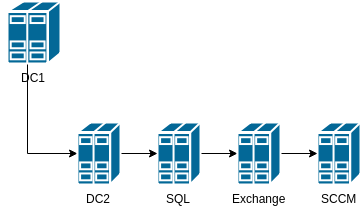
\includegraphics[width=8cm]{Netwerkdiagram.png}
\end{center}

\section{Server Requirements}

\begin{enumerate}
\item DC1
    \begin{enumerate}
    \item RAM: 2048 MB
    \item HDD: 50 GB
    \item Netwerkadapters: NAT en Internal Network (jenduf.gent)
            \begin{enumerate}
            \item NAT
            \end{enumerate}
            \begin{enumerate}
            \item IP: 192.168.1.1
            \item SN: 255.255.255.0
            \end{enumerate}
    \item OS Version: Windows Server 2016 
    \end{enumerate}
    
\clearpage

\item DC2
    \begin{enumerate}
    \item RAM: 2048 MB
    \item HDD: 50 GB
    \item Netwerkadapters: Internal Network (jenduf.gent)
            \begin{enumerate}
            \item IP: 192.168.1.2
            \item SN: 255.255.255.0
            \item DG: 192.168.1.1
            \end{enumerate}
    \item OS Version: Windows Server 2016 
    \end{enumerate}
    
\item SQL Server
    \begin{enumerate}
    \item RAM: 2048 MB
    \item HDD: 50 GB
    \item Netwerkadapters: Internal Network (jenduf.gent)
            \begin{enumerate}
            \item IP: 192.168.1.3
            \item SN: 255.255.255.0
            \item DG: 192.168.1.1
            \end{enumerate}
    \item OS Version: Windows Server 2016
    \item SQL Version: SQL Server 2013-2016
    \end{enumerate}
\item Exchange Server
    \begin{enumerate}
    \item RAM: 8096 MB
    \item HDD: 100 GB
    \item Netwerkadapters: Internal Network (jenduf.gent)
            \begin{enumerate}
            \item IP: 192.168.1.4
            \item SN: 255.255.255.0
            \item DG: 192.168.1.1
            \end{enumerate}
    \item OS Version: Windows Server 2016
    \item Exchange Version: Exchange Server 2013-2016
    \end{enumerate}
\item SCCM Server
    \begin{enumerate}
    \item RAM: 8089 MB
    \item HDD: 100 GB
    \item Netwerkadapters: Internal Network (jenduf.gent)
            \begin{enumerate}
            \item IP: 192.168.1.5
            \item SN: 255.255.255.0
            \item DG: 192.168.1.1
            \end{enumerate}
    \item OS Version: Windows Server 2016
    \item OS Version: Windows Deployment Server 2012
    \end{enumerate}
\end{enumerate}

\section{Windows Server Installatie}
\begin{center}
	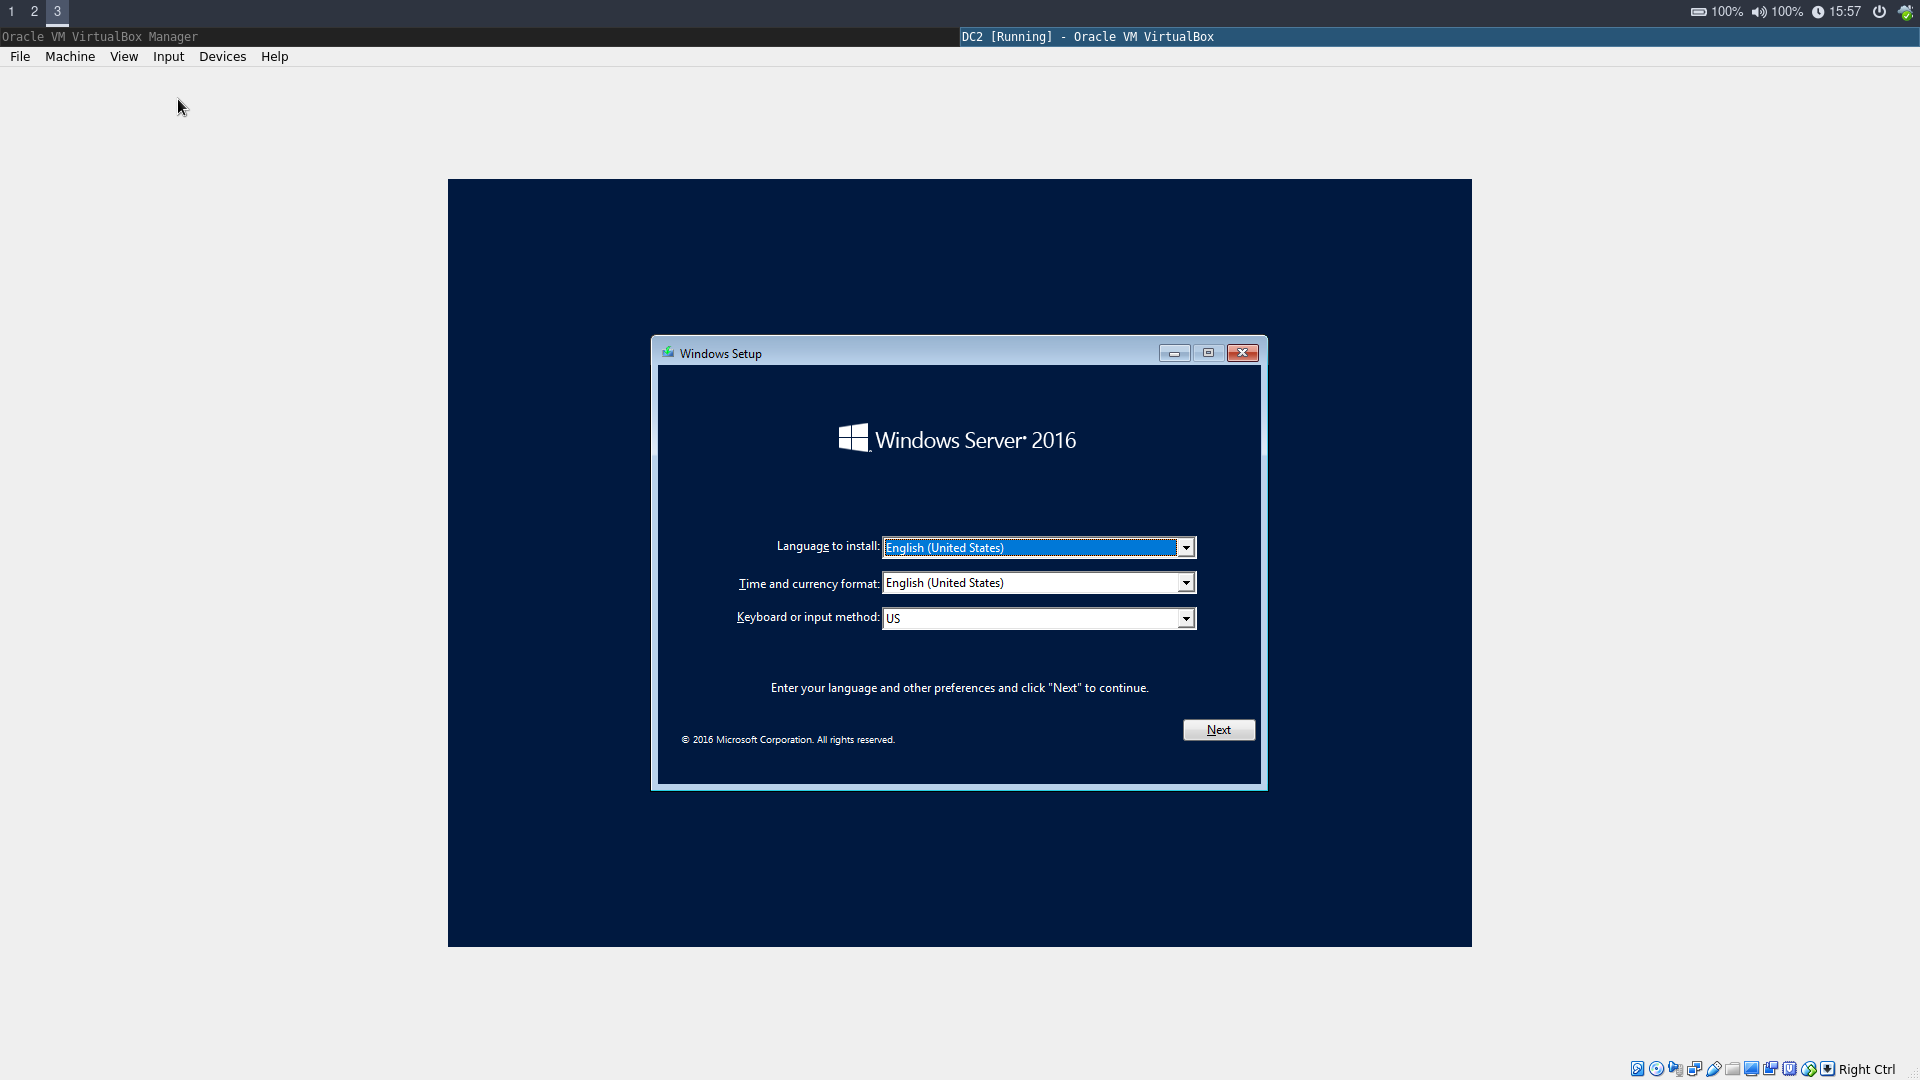
\includegraphics[width=15cm]{Pictures/Windows_Install/1542293852.png}
	Selecteer de gewenste taalinstellingen.
\end{center}
\begin{center}
	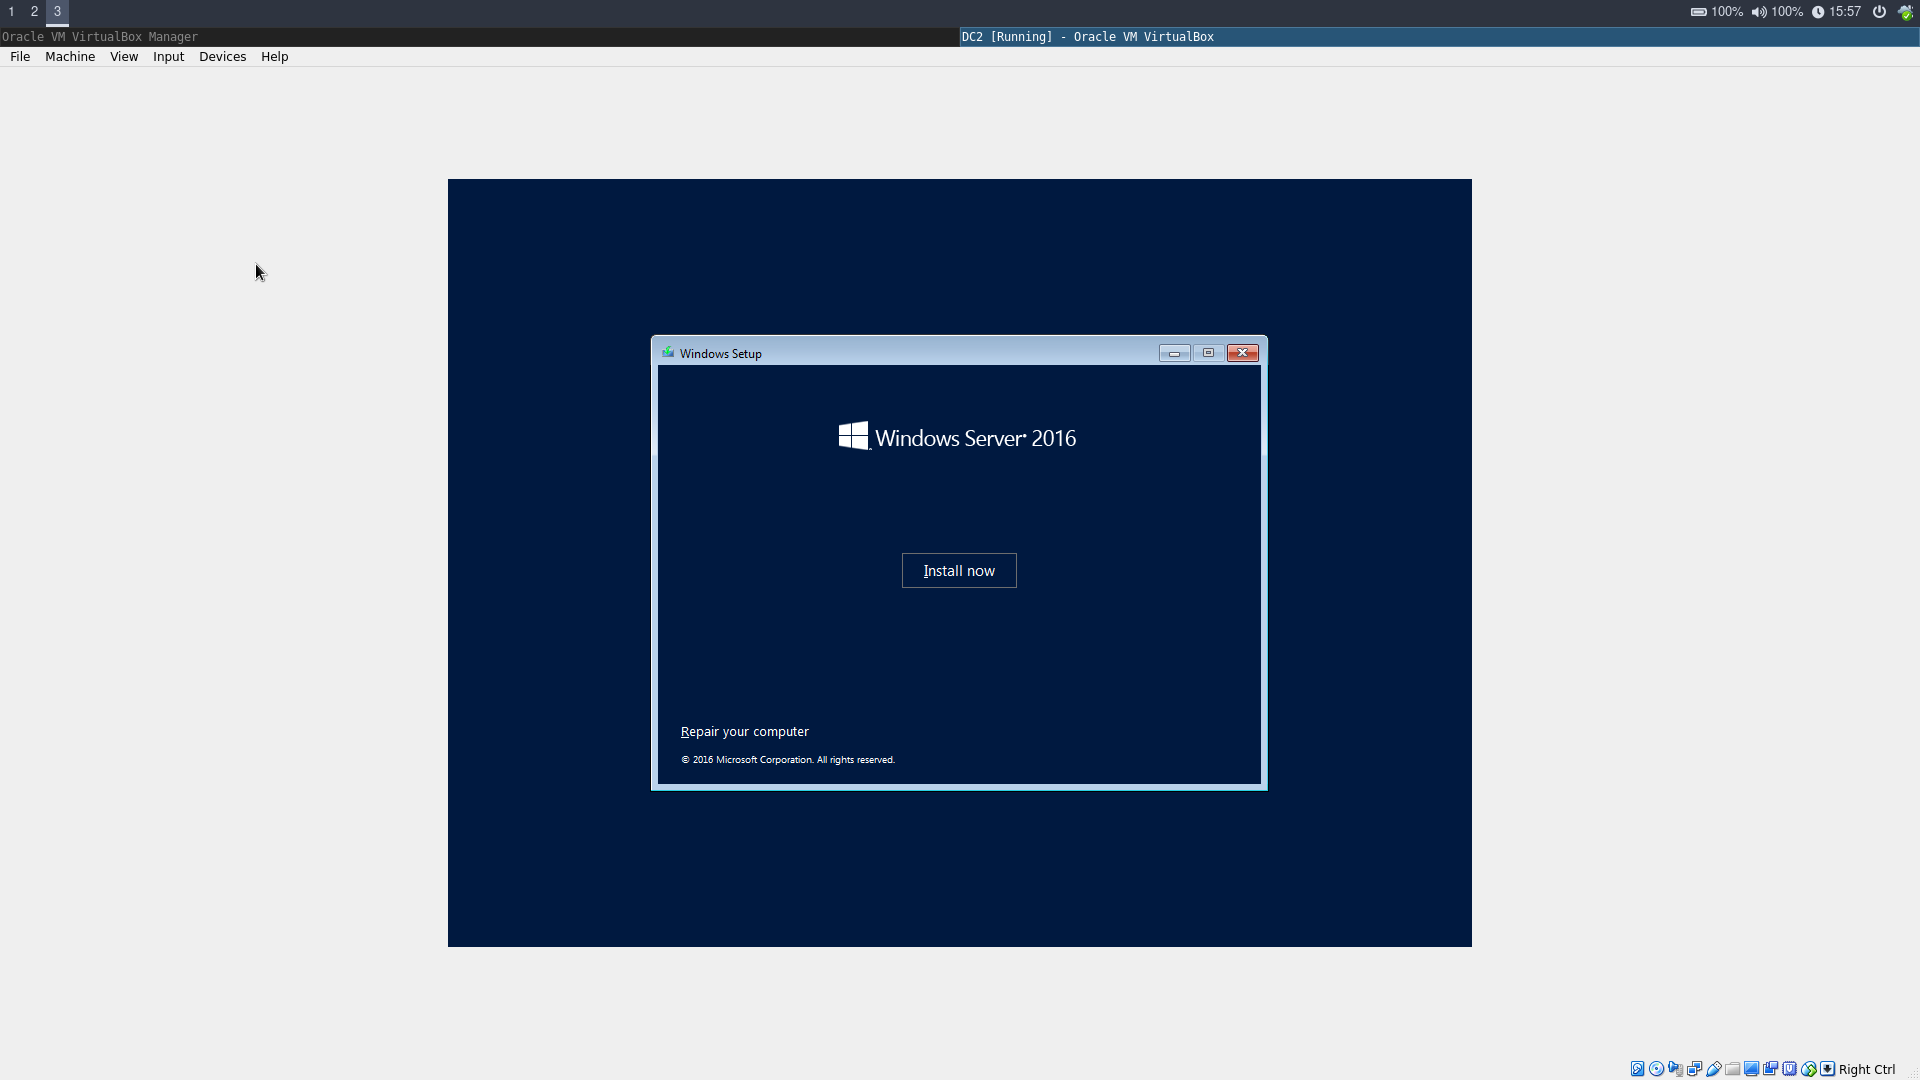
\includegraphics[width=15cm]{Pictures/Windows_Install/1542293872.png}
	
	Start de installatie.
\end{center}
\begin{center}
	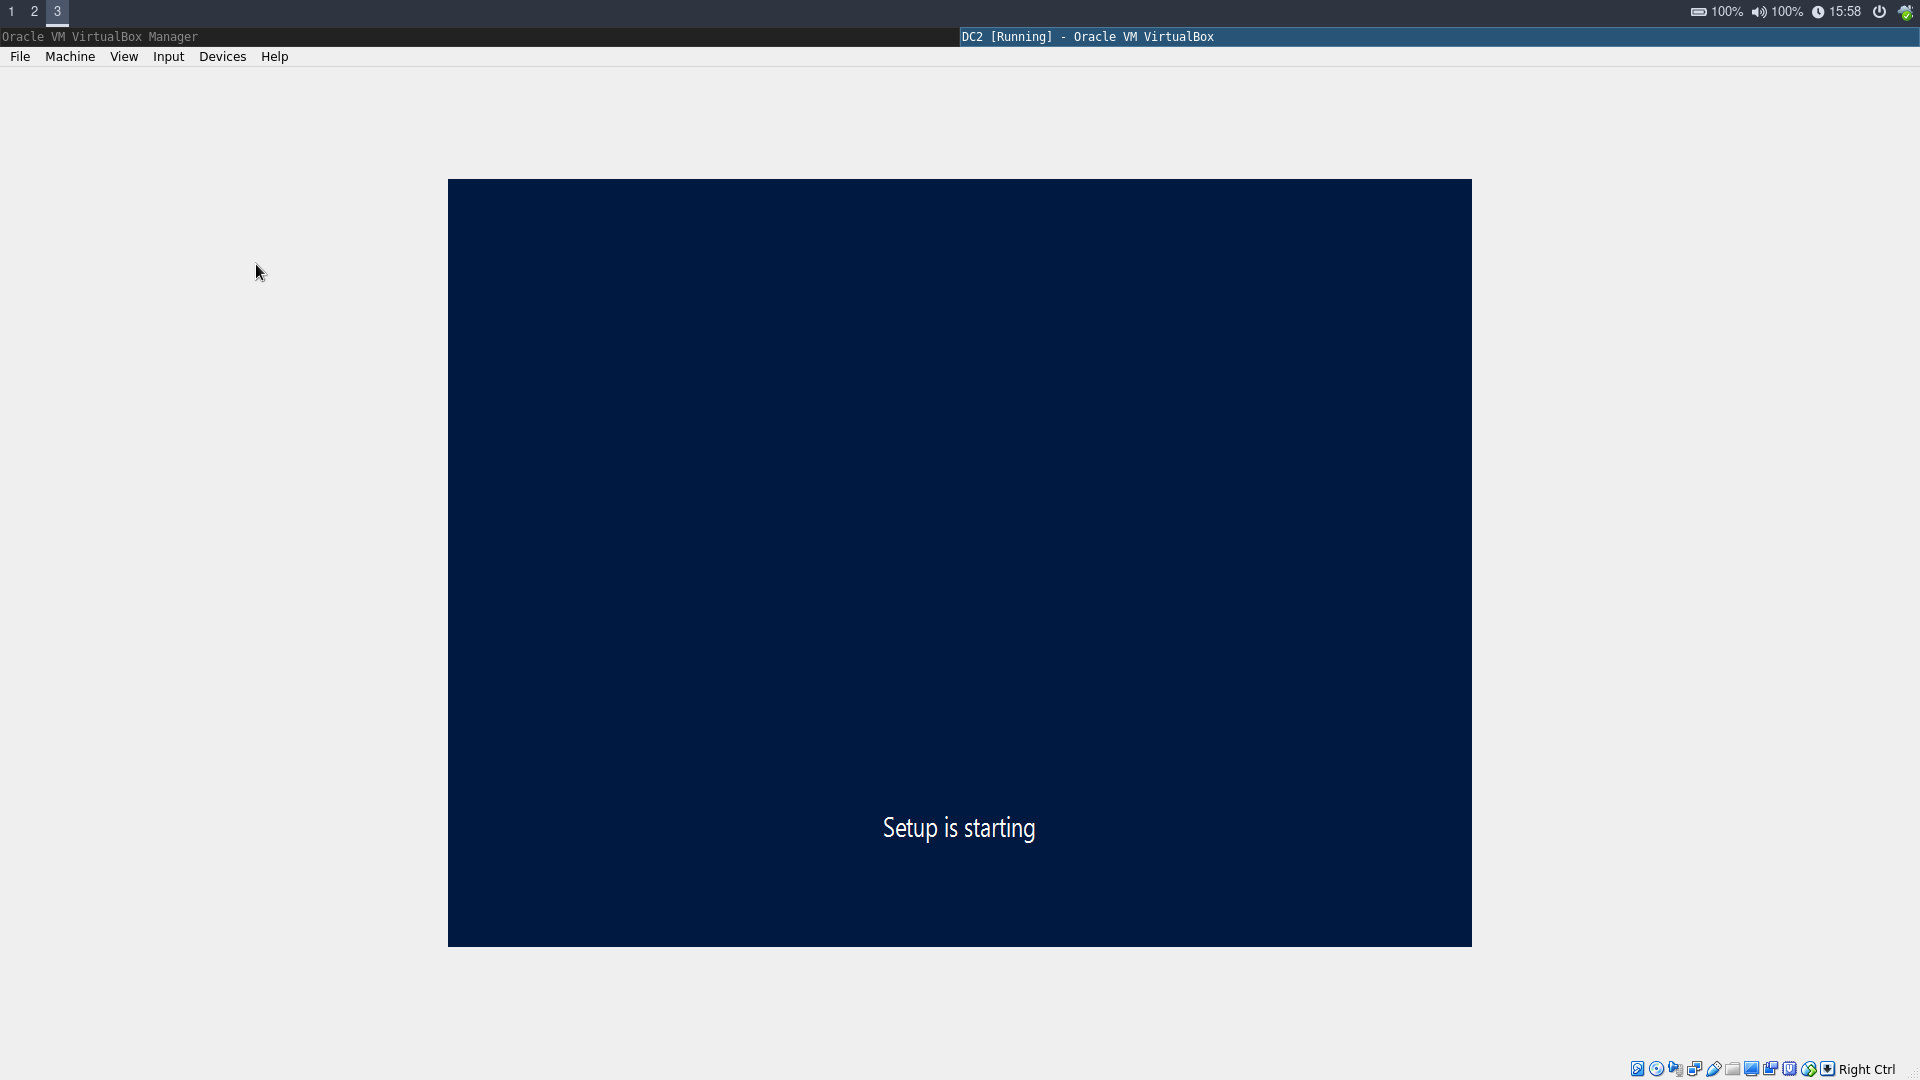
\includegraphics[width=15cm]{Pictures/Windows_Install/1542293887.png}
\end{center}
\begin{center}
	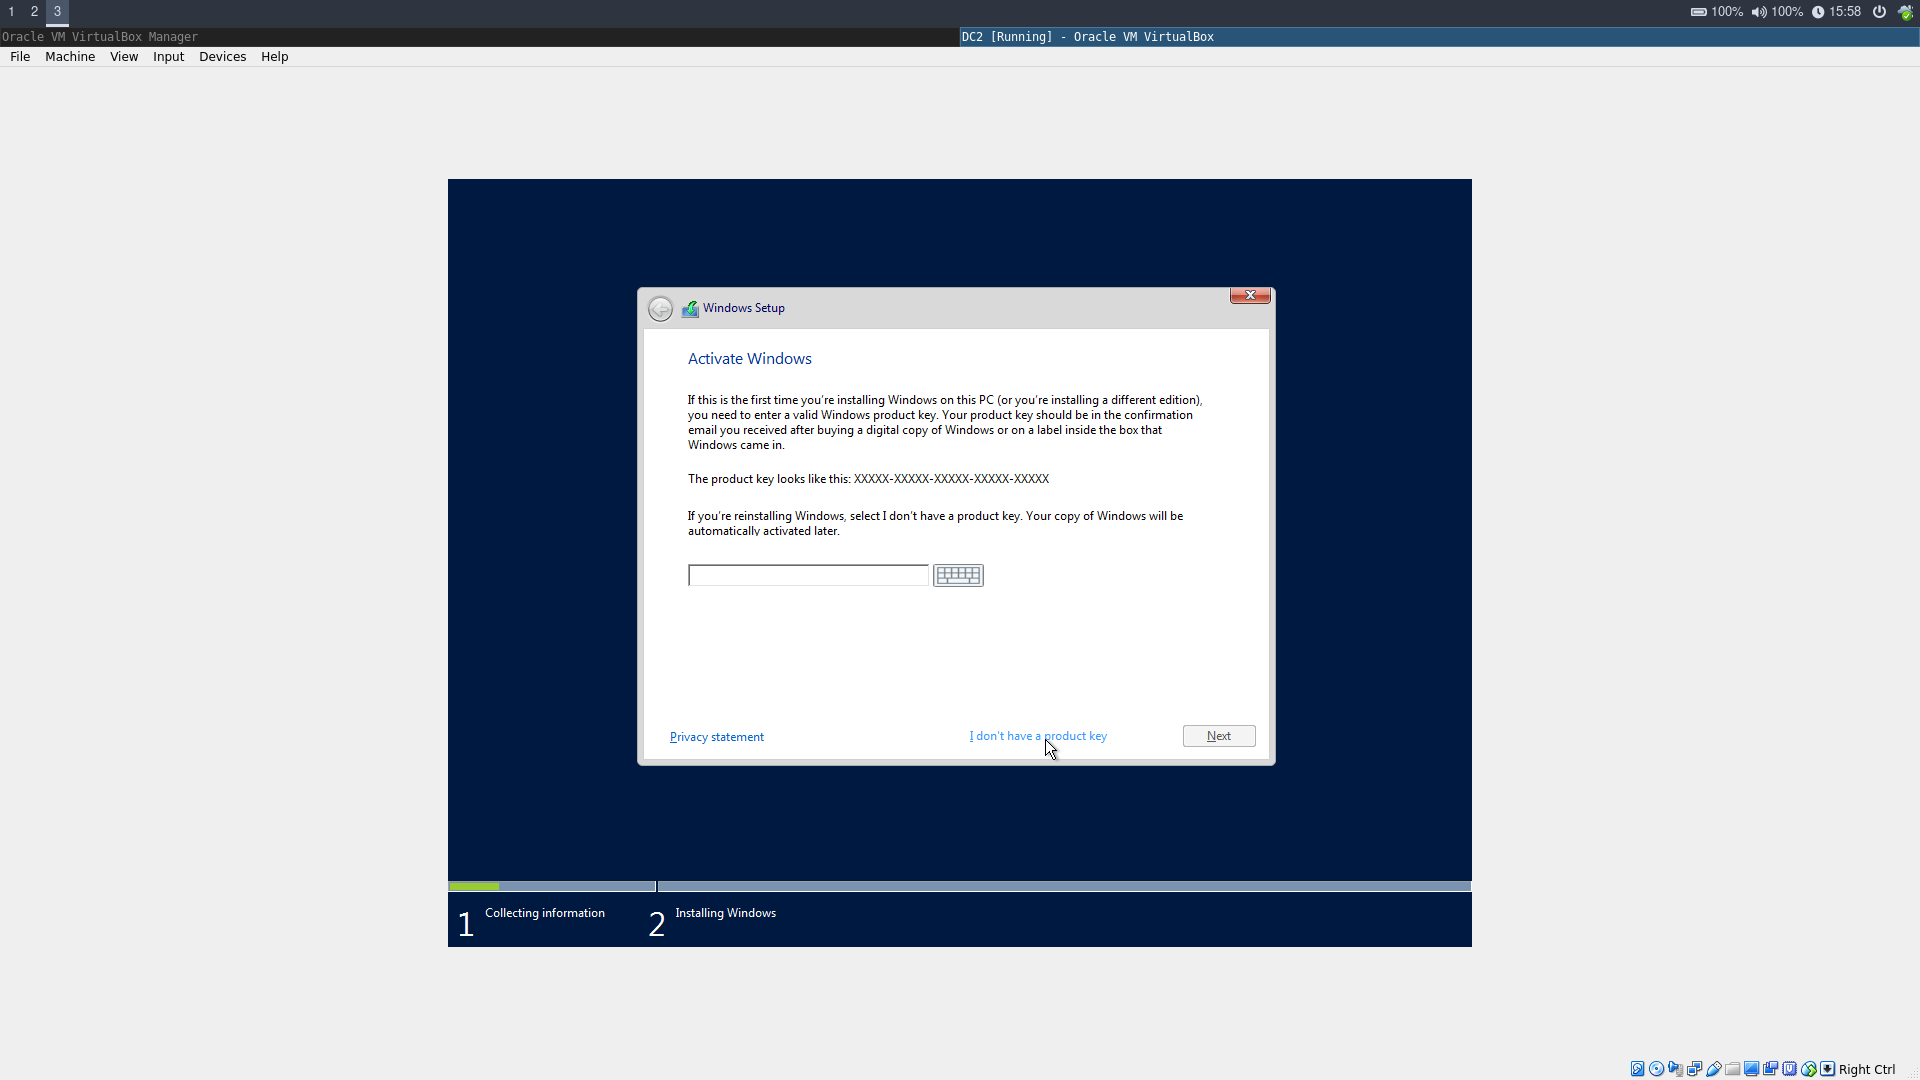
\includegraphics[width=15cm]{Pictures/Windows_Install/1542293899.png}
	
	Selecteer "I don't have a product key".
\end{center}
\begin{center}
	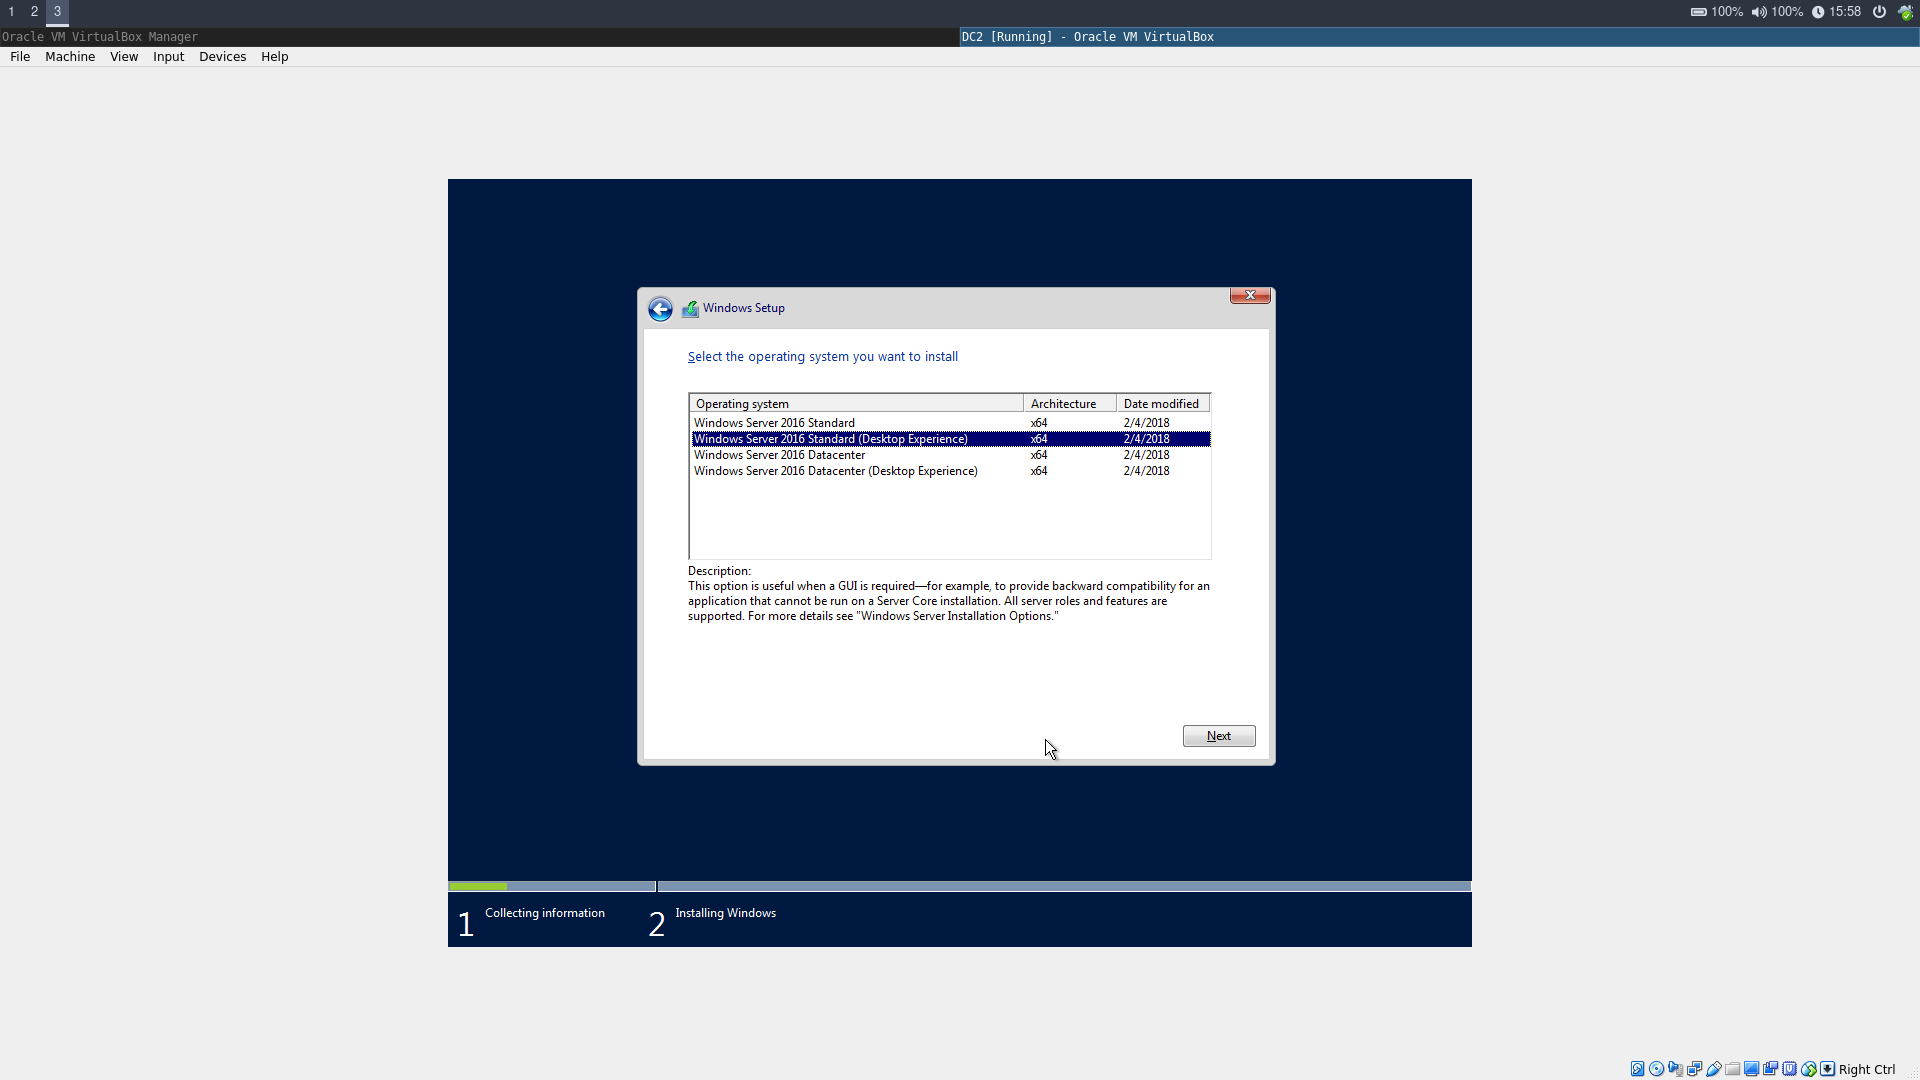
\includegraphics[width=15cm]{Pictures/Windows_Install/1542293908.png}
	
	Selecteer "Windows Server 2016 Standard (Desktop Experience)".
\end{center}
\begin{center}
	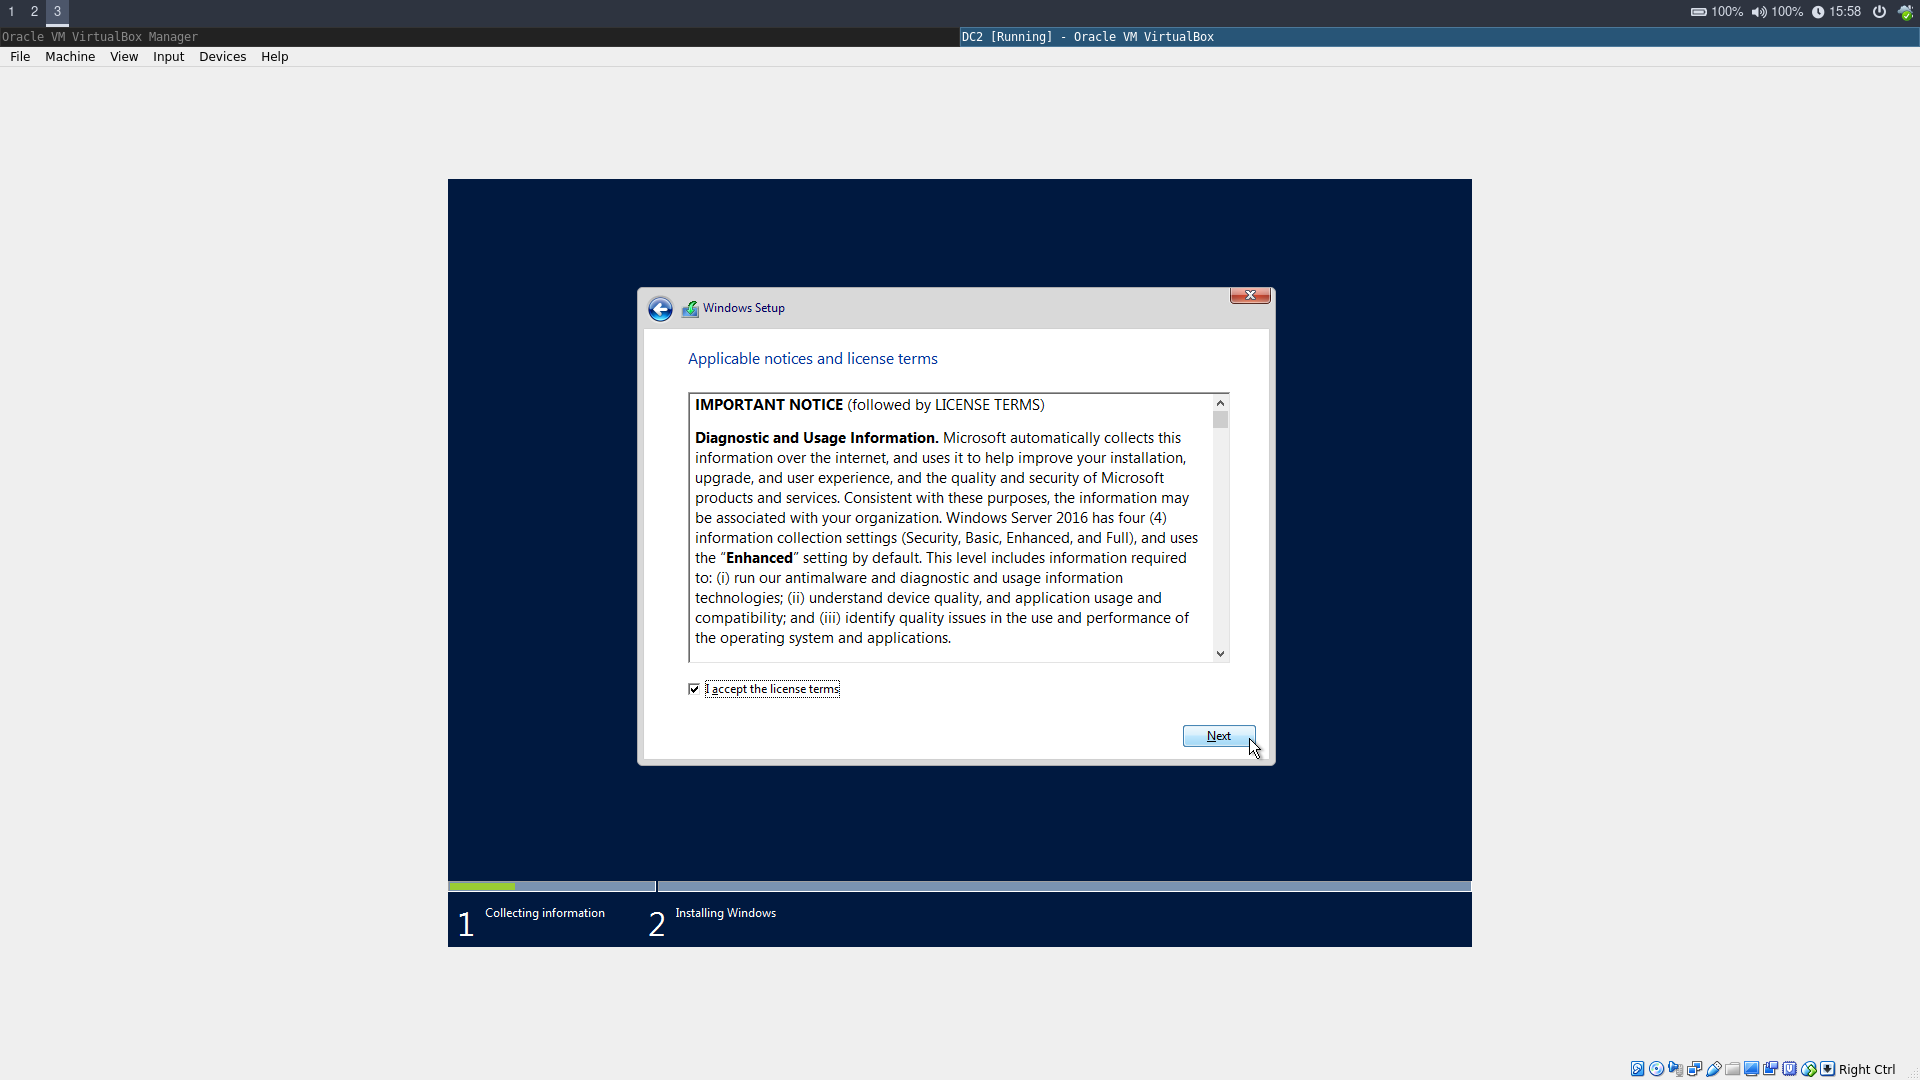
\includegraphics[width=15cm]{Pictures/Windows_Install/1542293921.png}
	
	Ga akkoord met de gebruiksvoorwaarden.
\end{center}
\begin{center}
	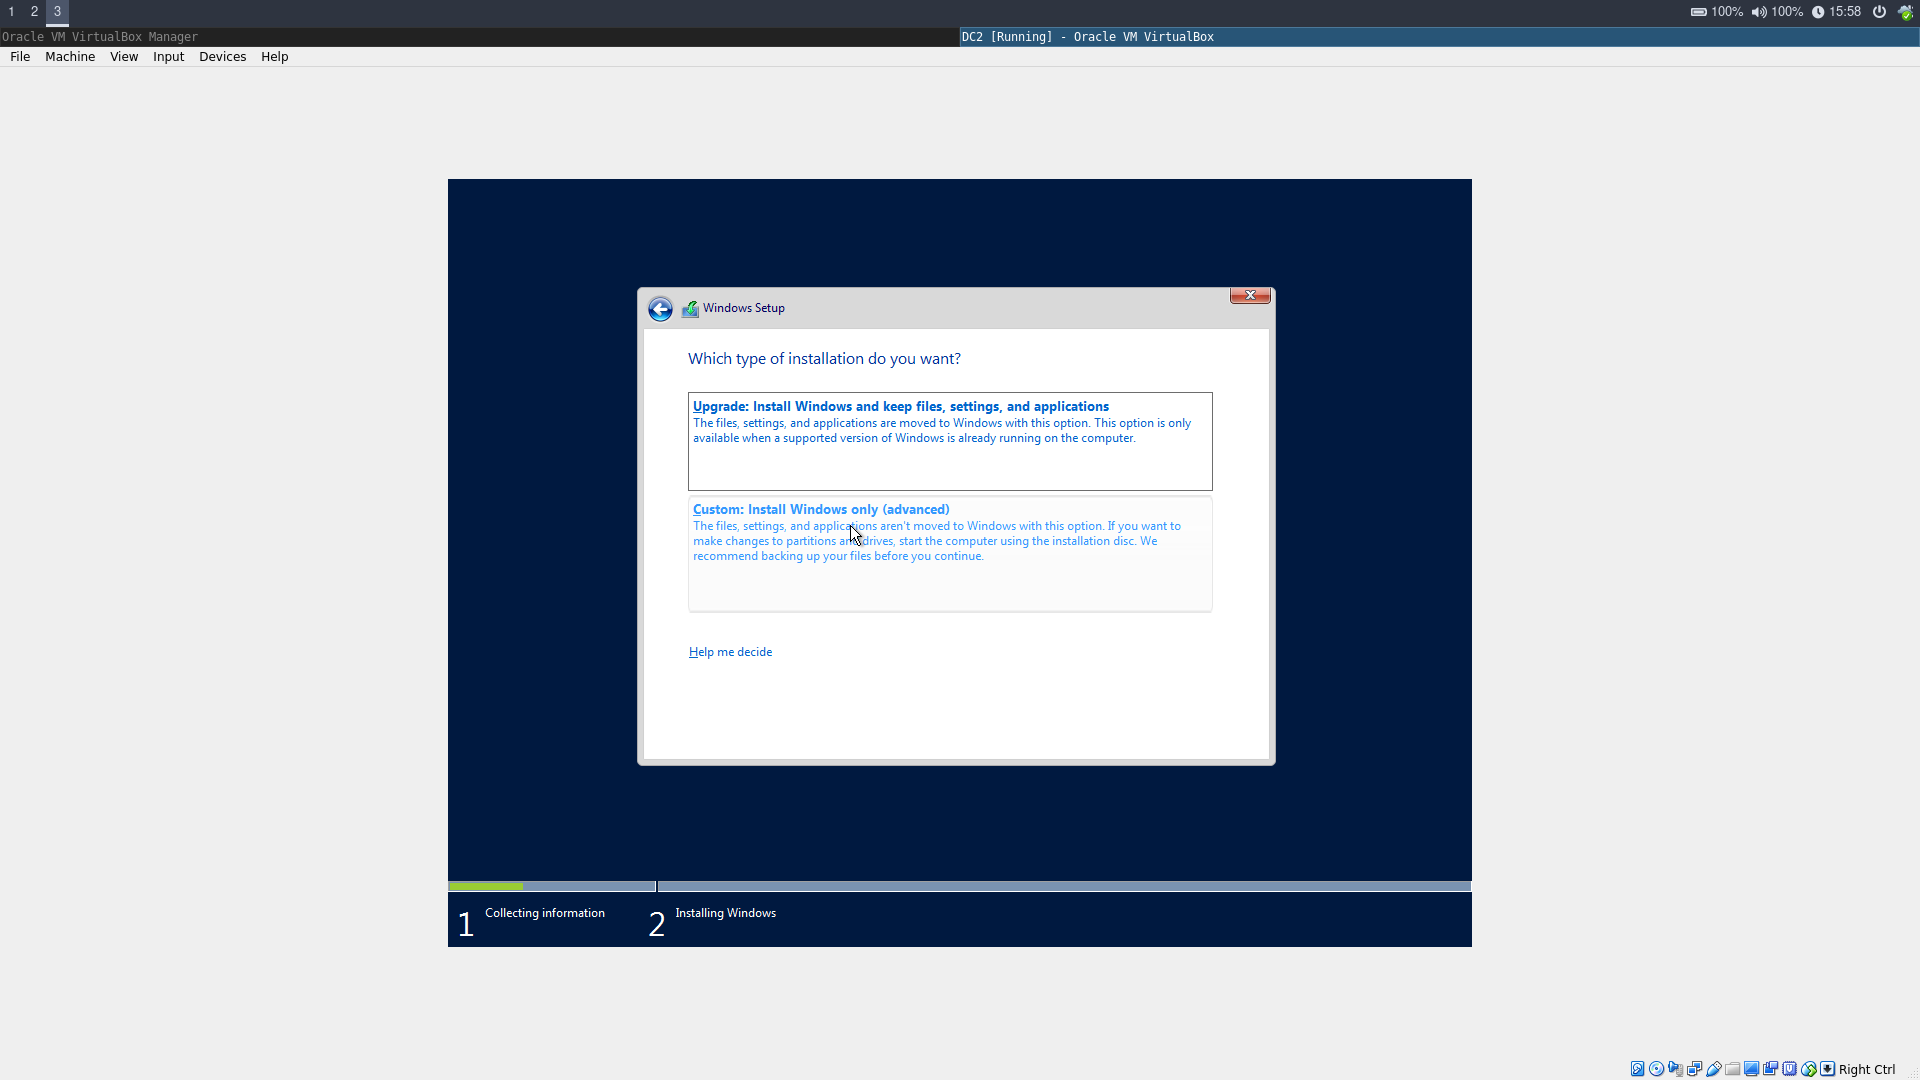
\includegraphics[width=15cm]{Pictures/Windows_Install/1542293929.png}
	
	Selecteer "Costum: Install Windows only (Advanced)".
\end{center}
\begin{center}
	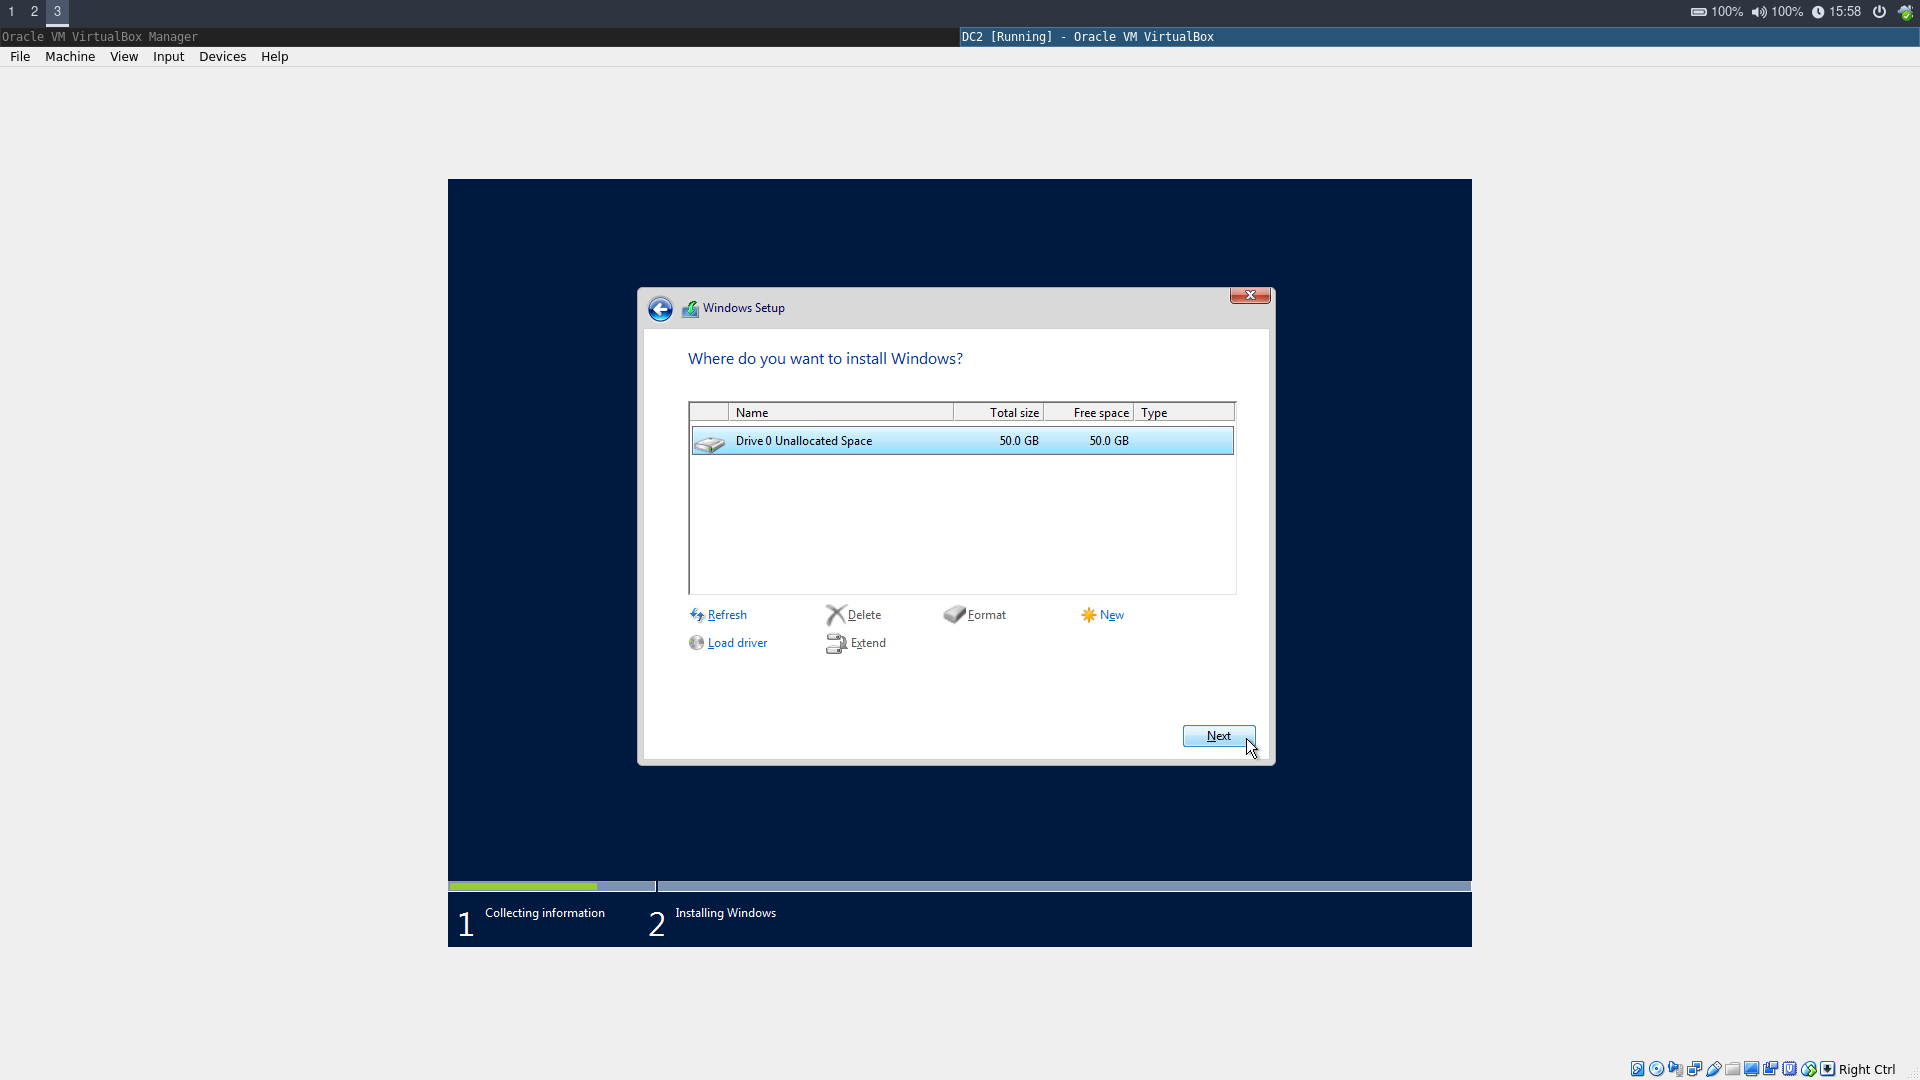
\includegraphics[width=15cm]{Pictures/Windows_Install/1542293934.png}
	
	Ga verder.
\end{center}
\begin{center}
	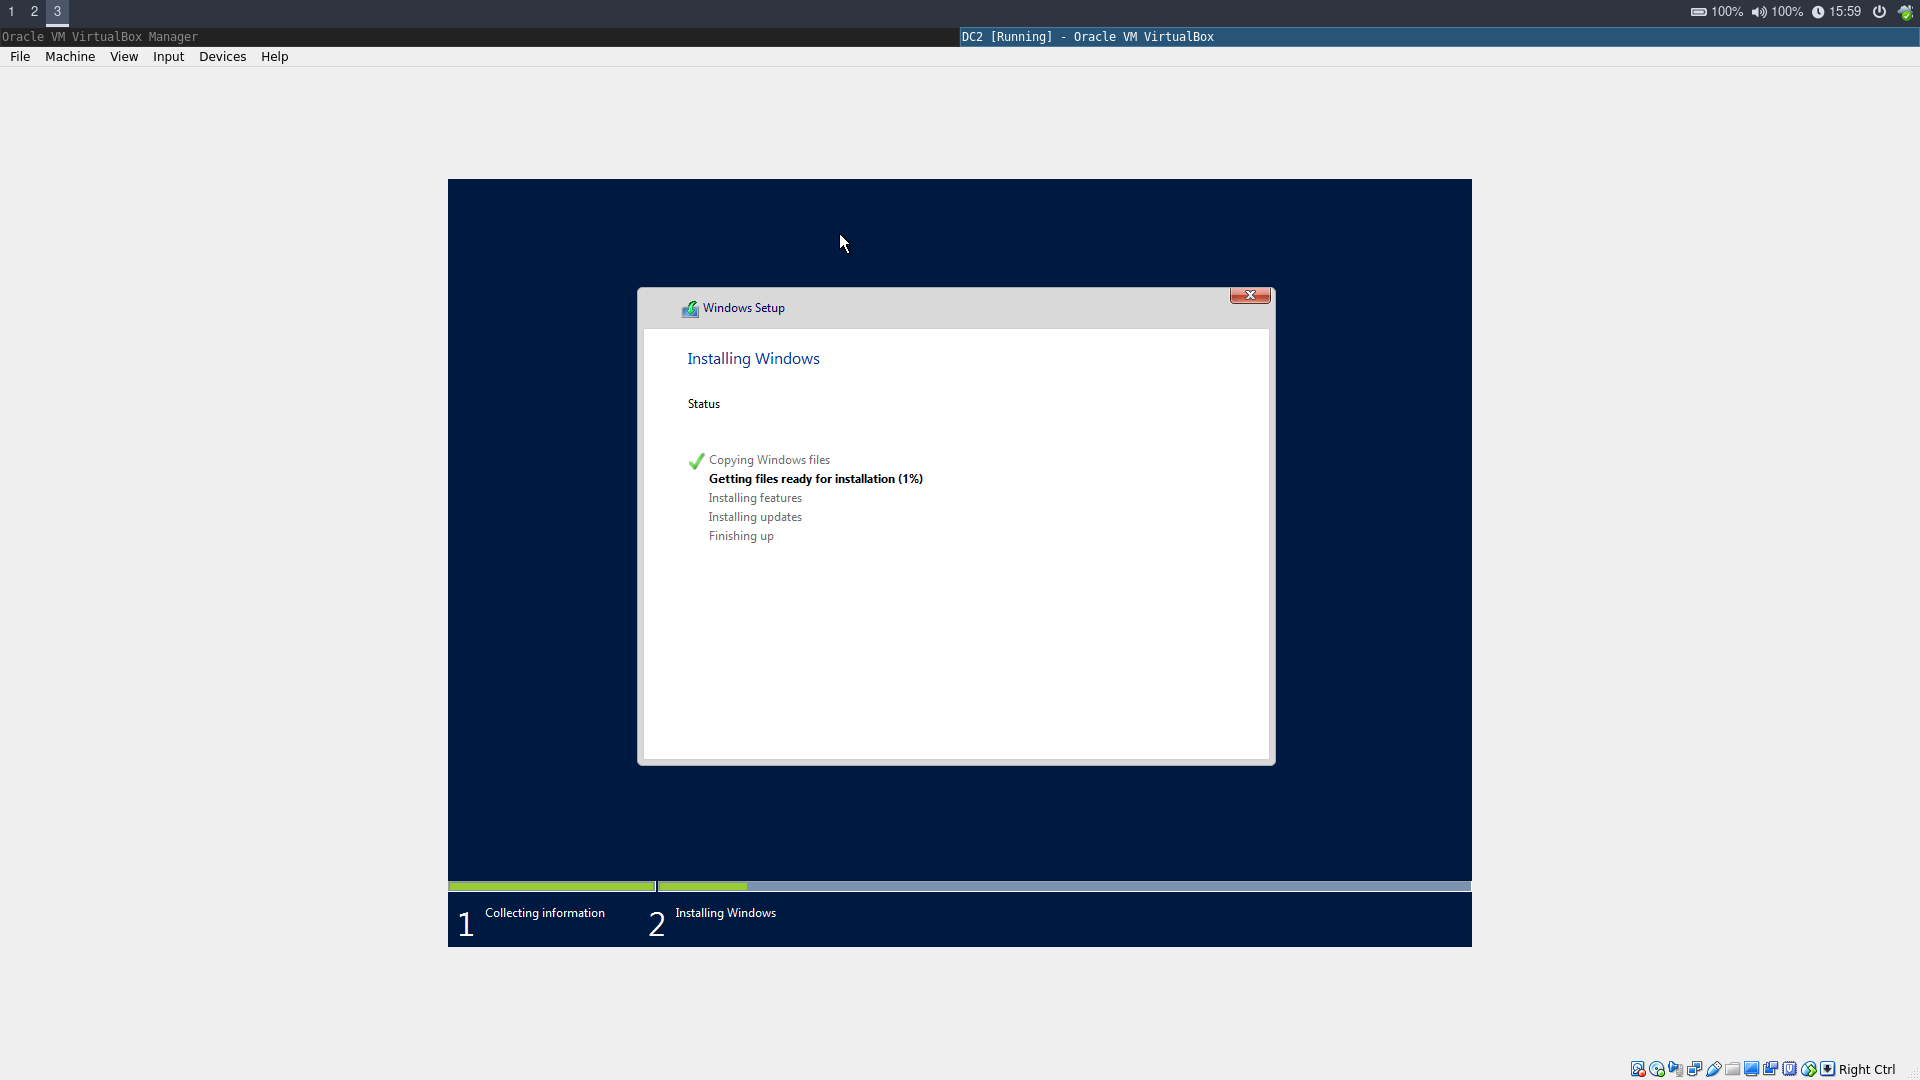
\includegraphics[width=15cm]{Pictures/Windows_Install/1542293945.png}
\end{center}
\subsection{Server Hernoemen}
\begin{center}
	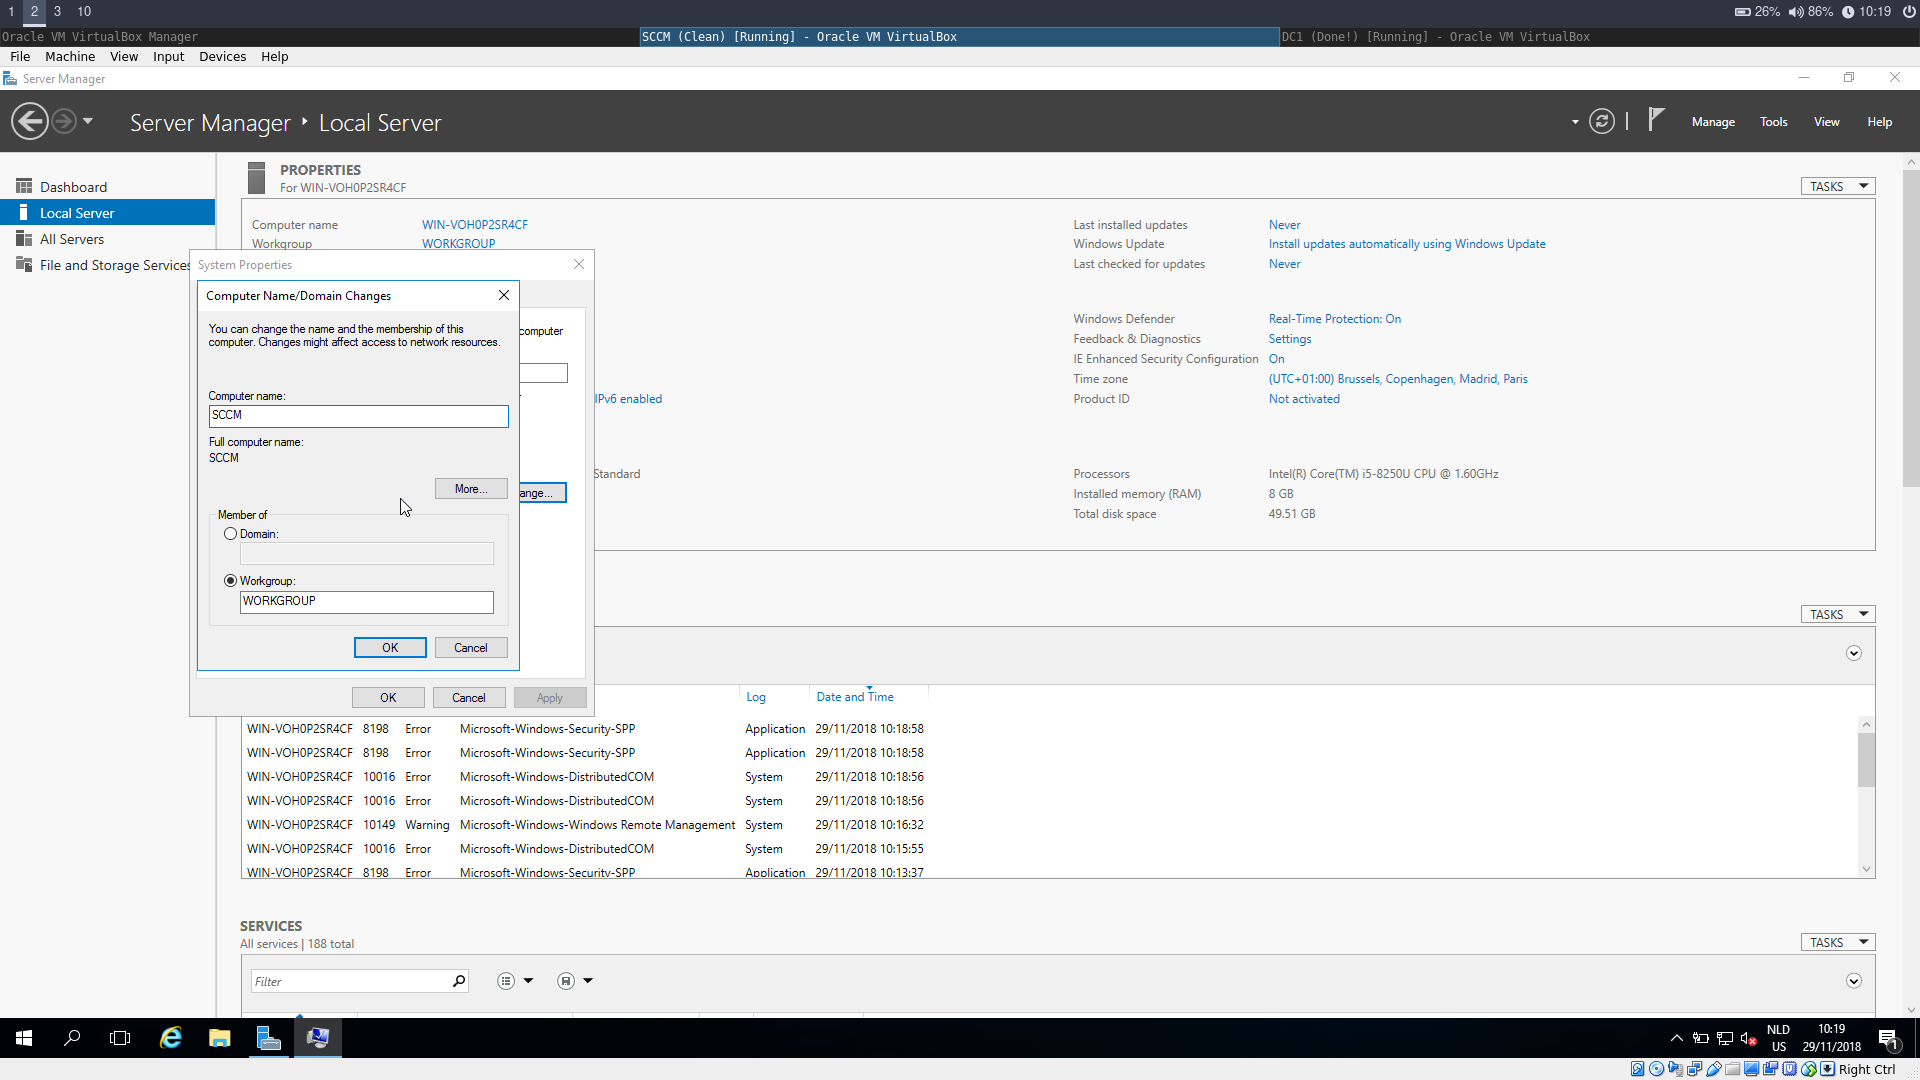
\includegraphics[width=15cm]{Pictures/SCCM/0/1543483191.png}
\end{center}
\subsection{IP Instellingen}
\begin{center}
	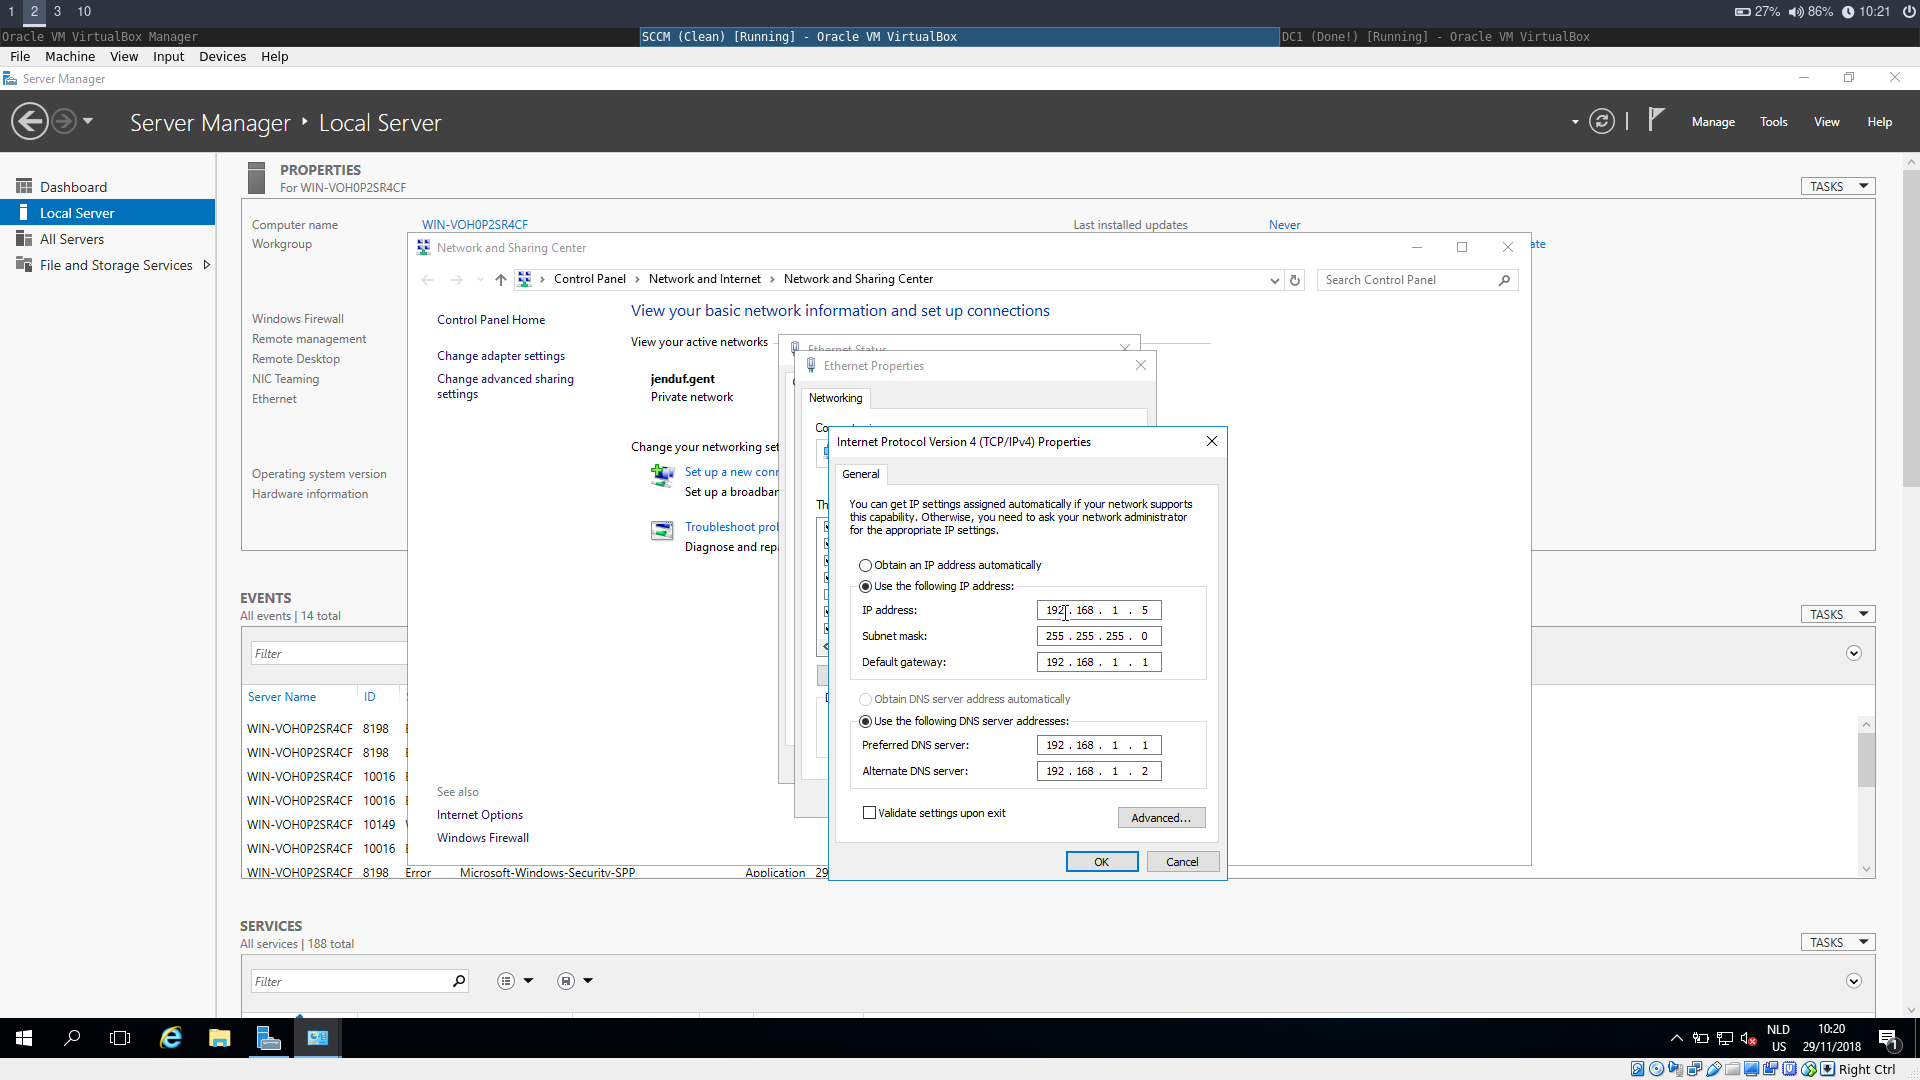
\includegraphics[width=15cm]{Pictures/SCCM/0/1543483265.png}
\end{center}
\subsection{Toevoegen aan het domein}
\begin{center}
	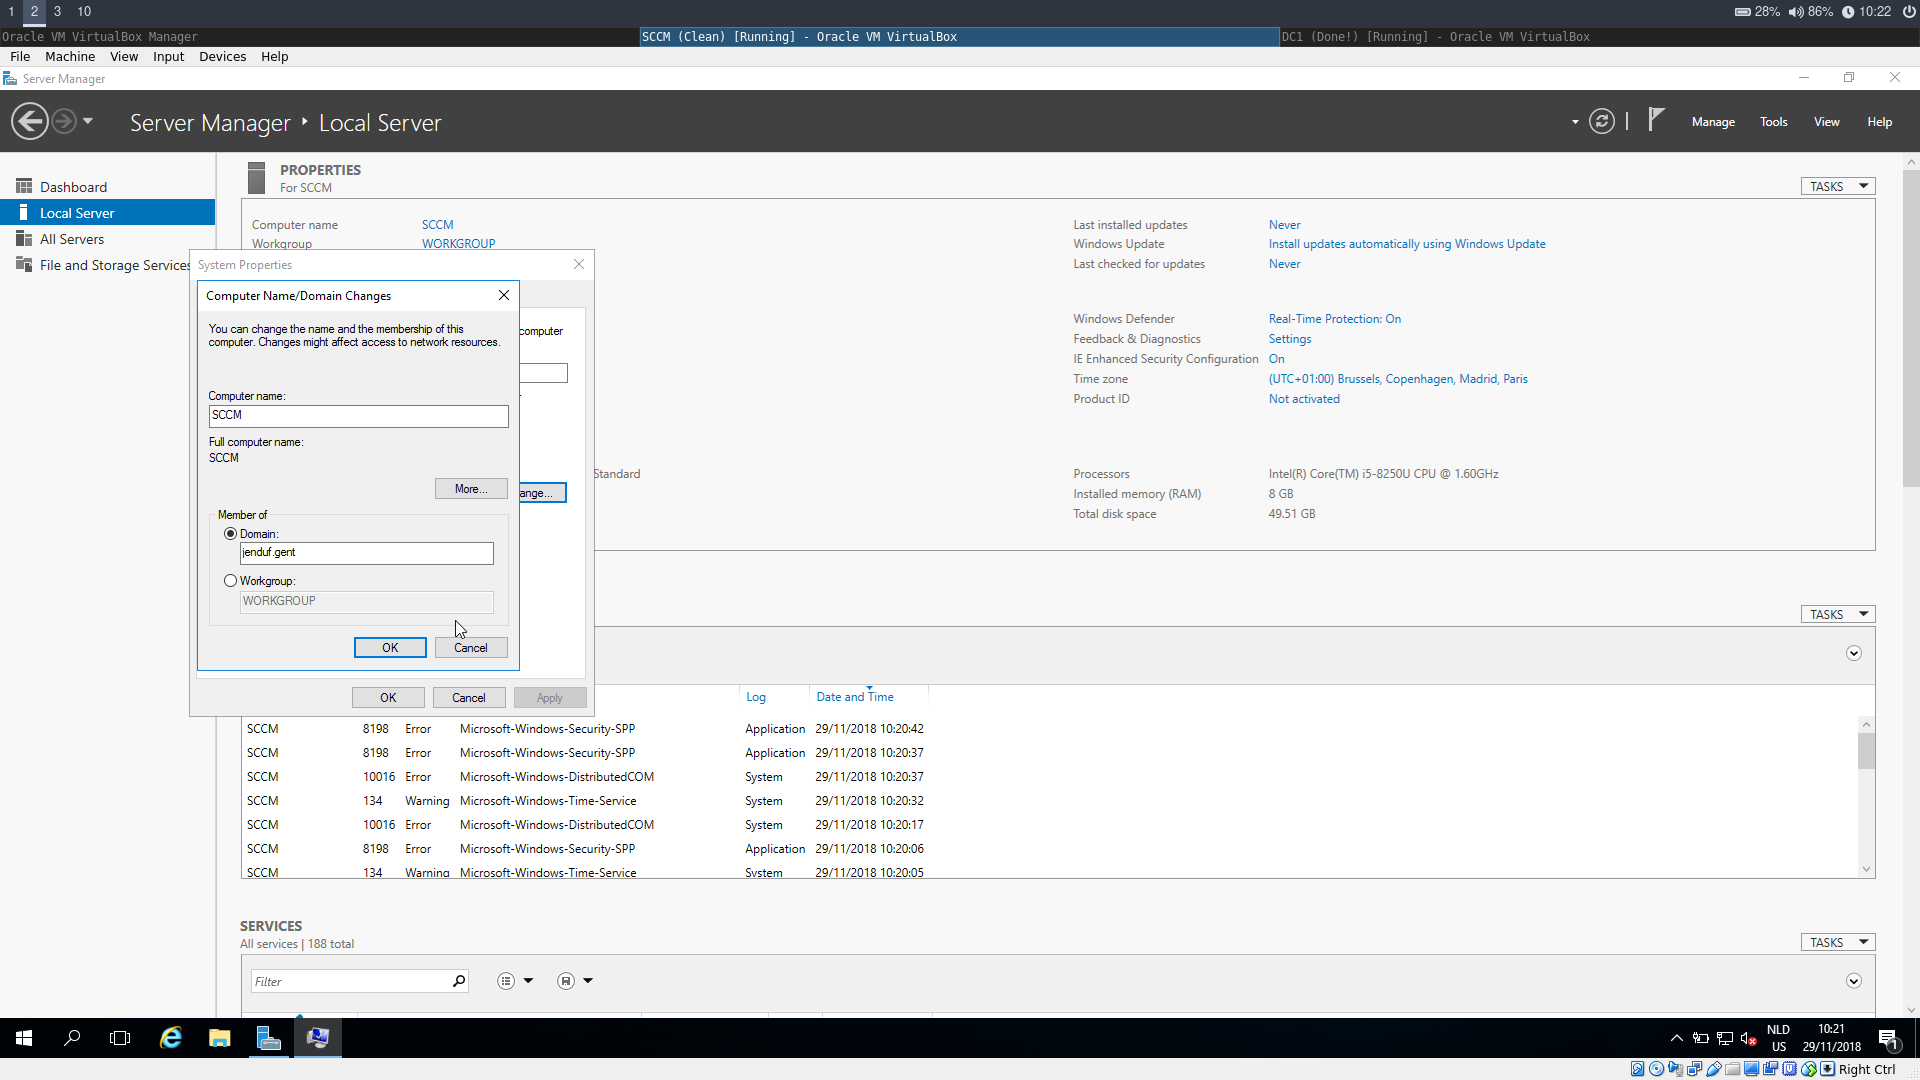
\includegraphics[width=15cm]{Pictures/SCCM/0/1543483352.png}
	
	Geef als domein jenduf.gent in.
\end{center}
\begin{center}
	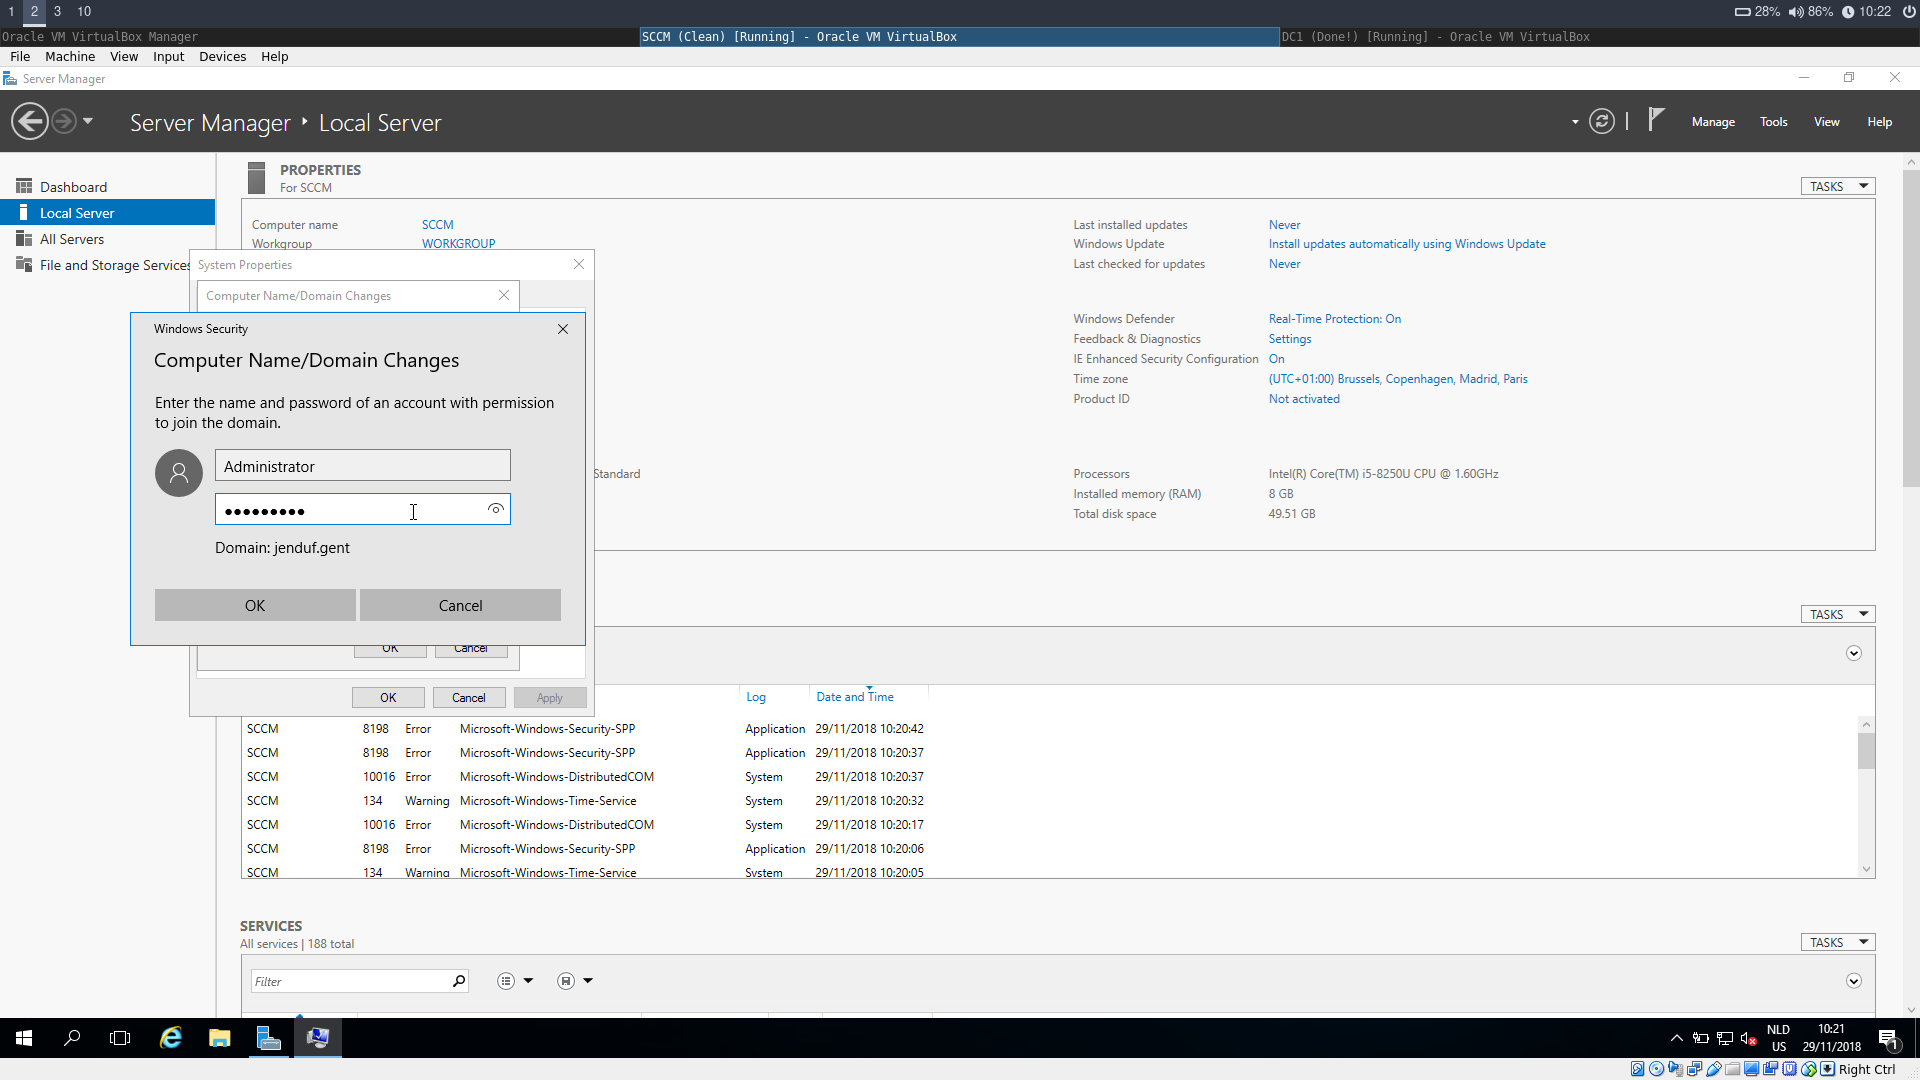
\includegraphics[width=15cm]{Pictures/SCCM/0/1543483358.png}
	
	Geef gebruikersnaam "Administrator" in en paswoord "Admin2018".
\end{center}
\begin{center}
	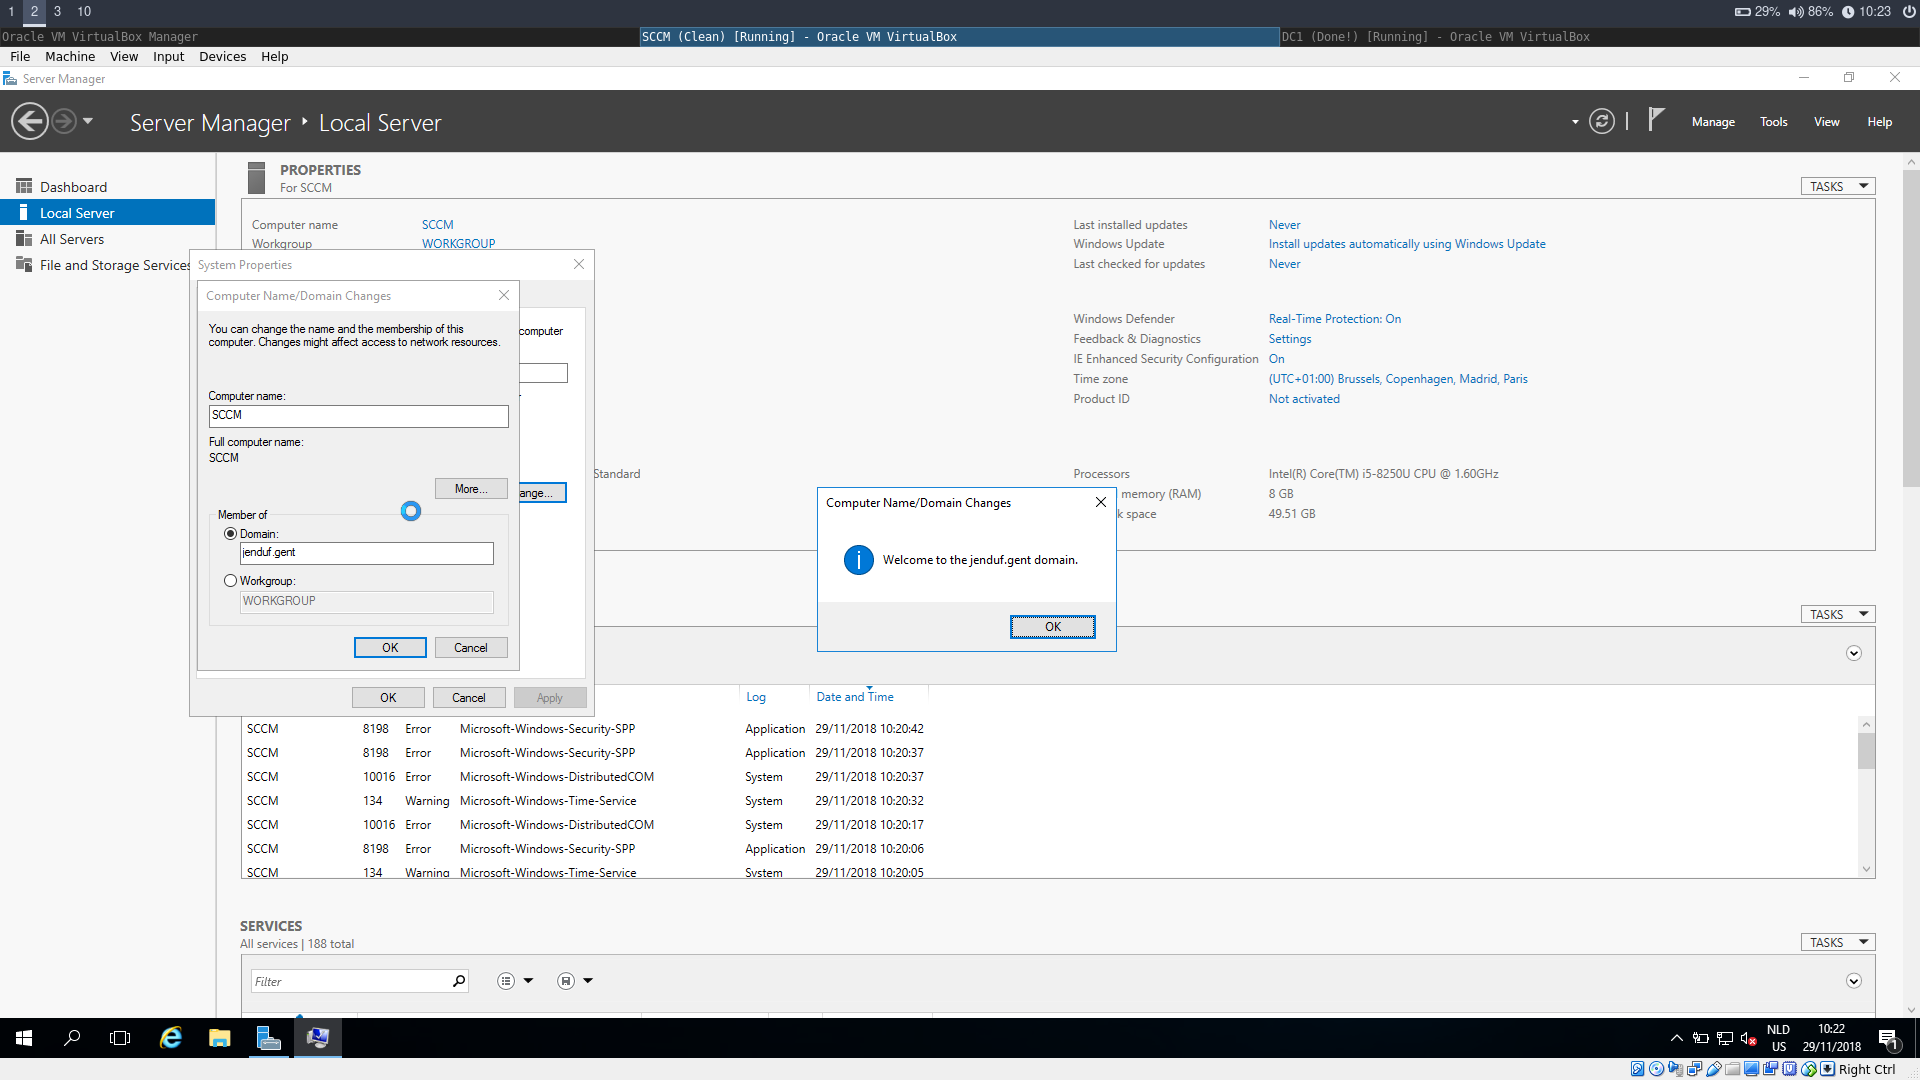
\includegraphics[width=15cm]{Pictures/SCCM/0/1543483399.png}
	
	De connectie is geslaagd bij het weergeven van volgende boodschap.
\end{center}

\clearpage



\section{Installatie SCCM}
\subsection{Prerequisites voor SCCM}
\begin{center}
	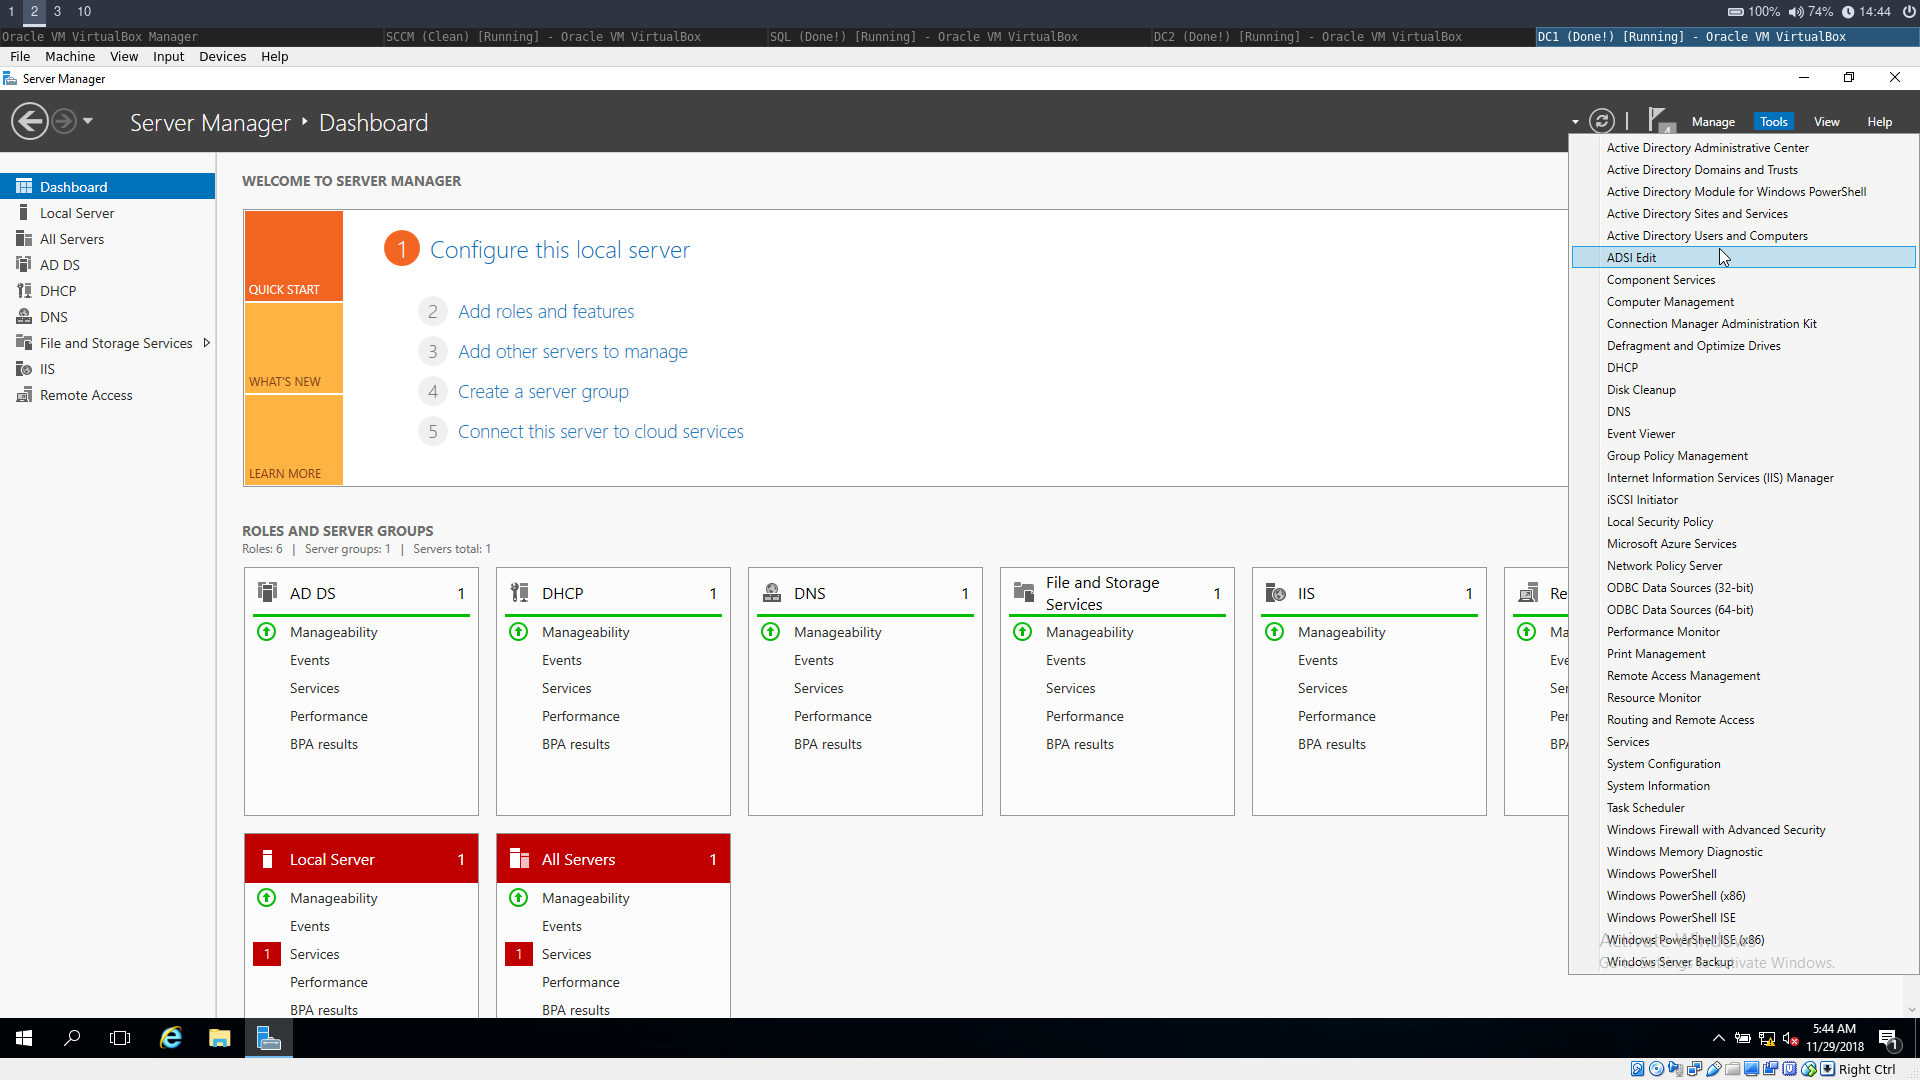
\includegraphics[width=15cm]{Pictures/SCCM/1/1543499067.png}
	
	Open "ADSI Edit".
\end{center}
\begin{center}
	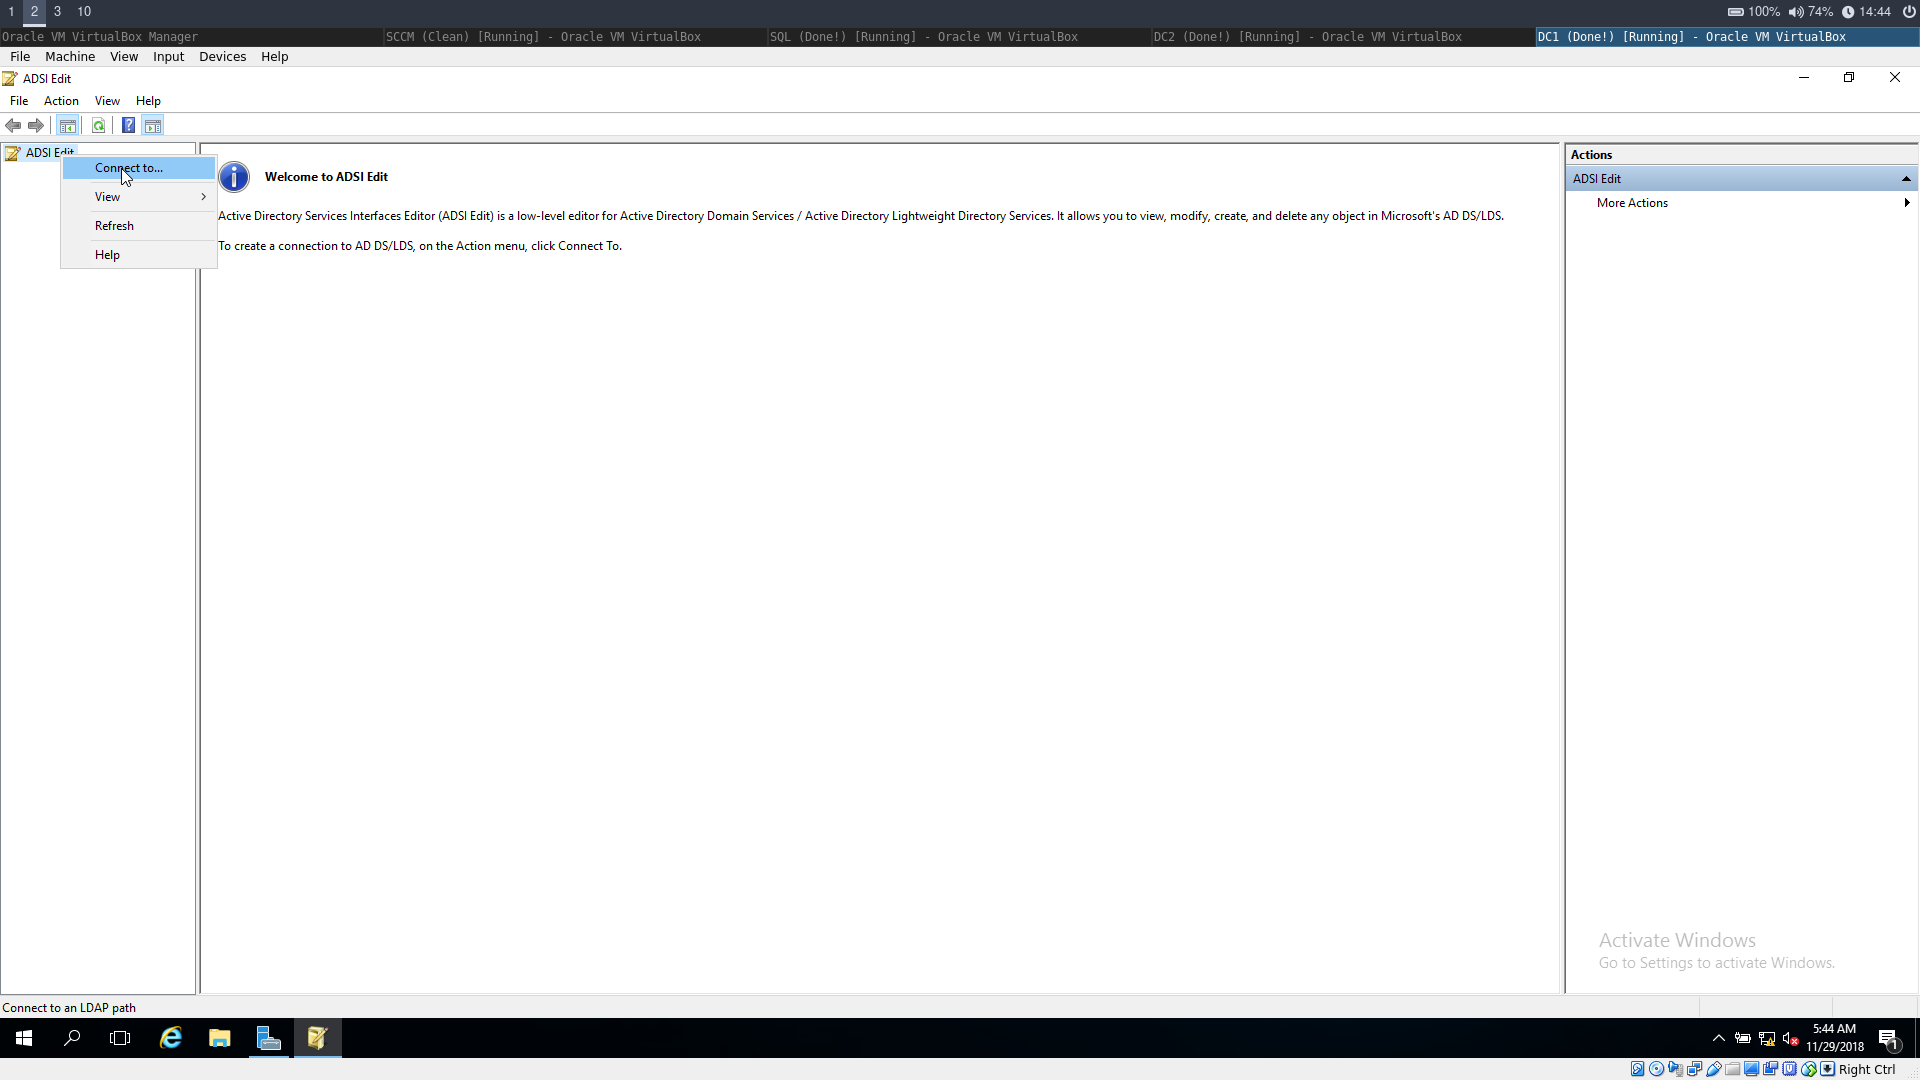
\includegraphics[width=15cm]{Pictures/SCCM/1/1543499073.png}
	
	Selecteer de optie "Connect to..."
\end{center}
\begin{center}
	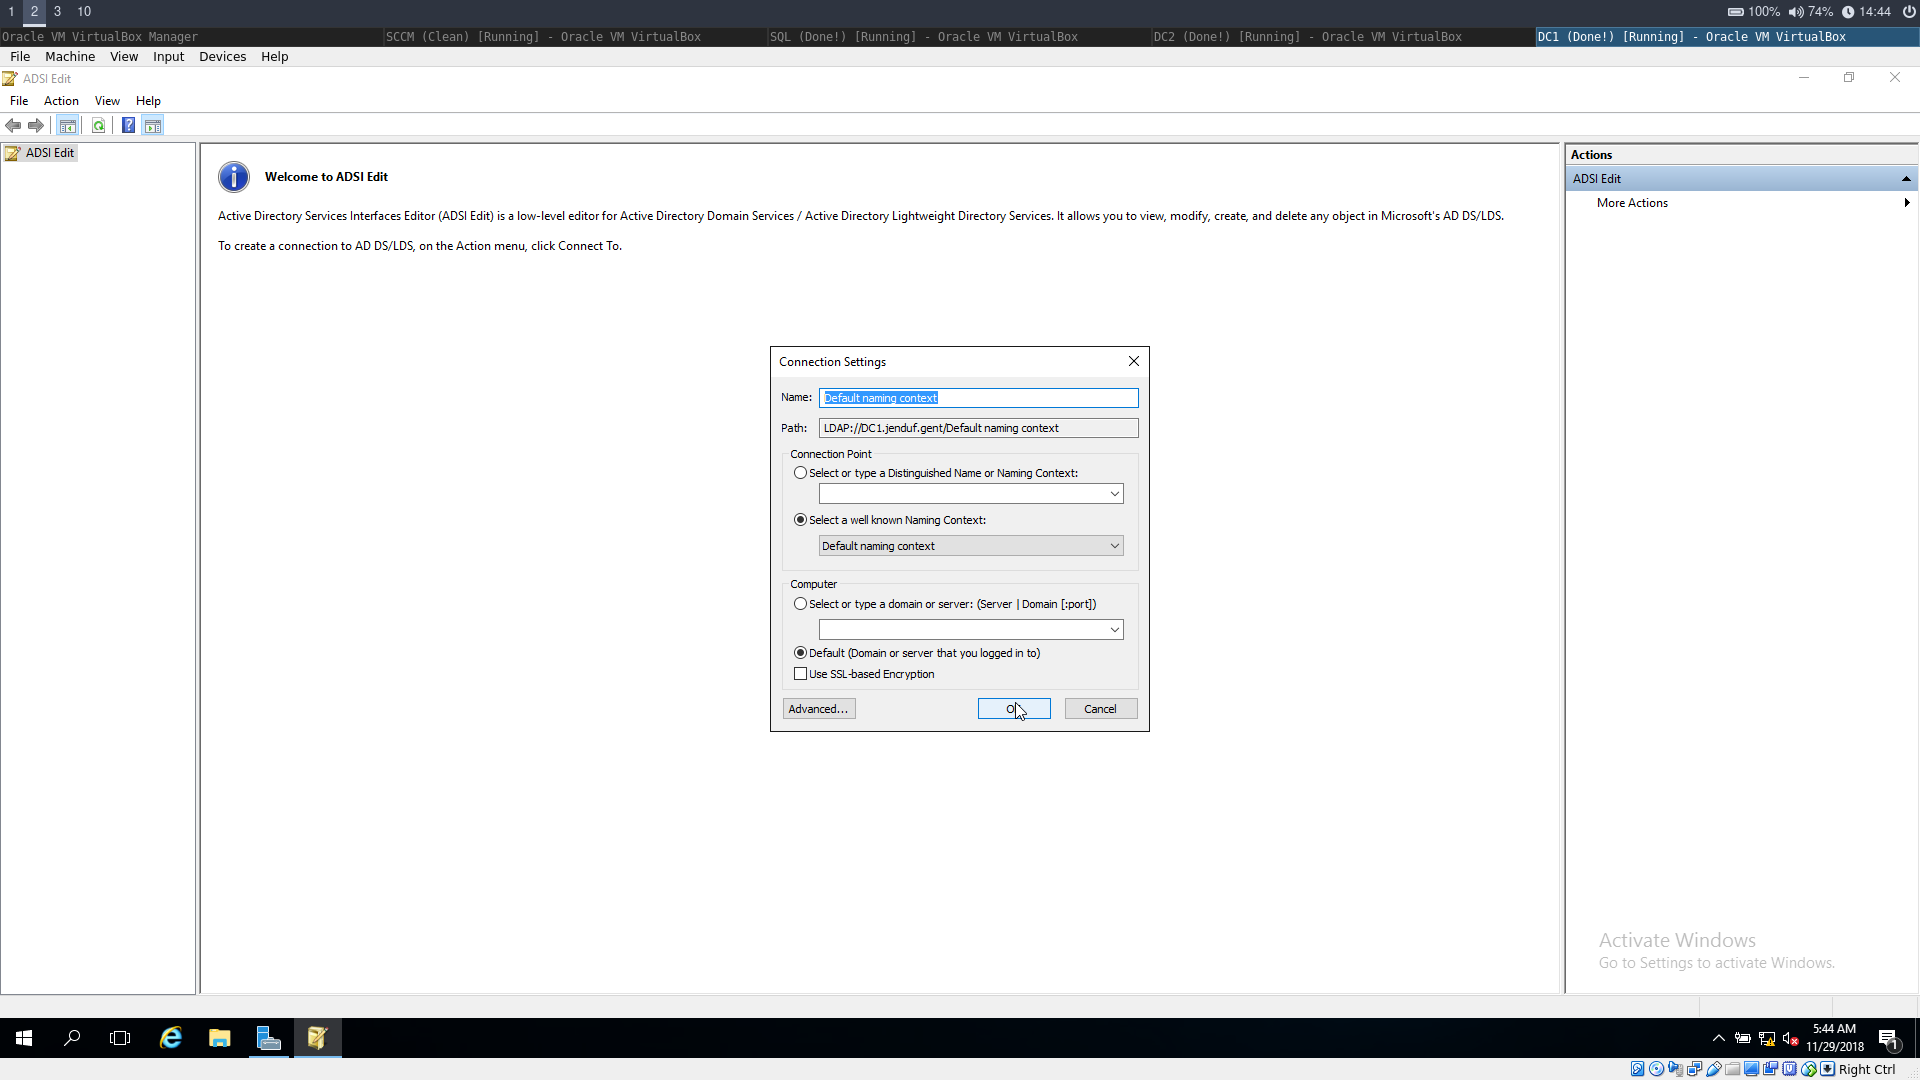
\includegraphics[width=15cm]{Pictures/SCCM/1/1543499076.png}
	
	Klik op "Ok".
\end{center}
\begin{center}
	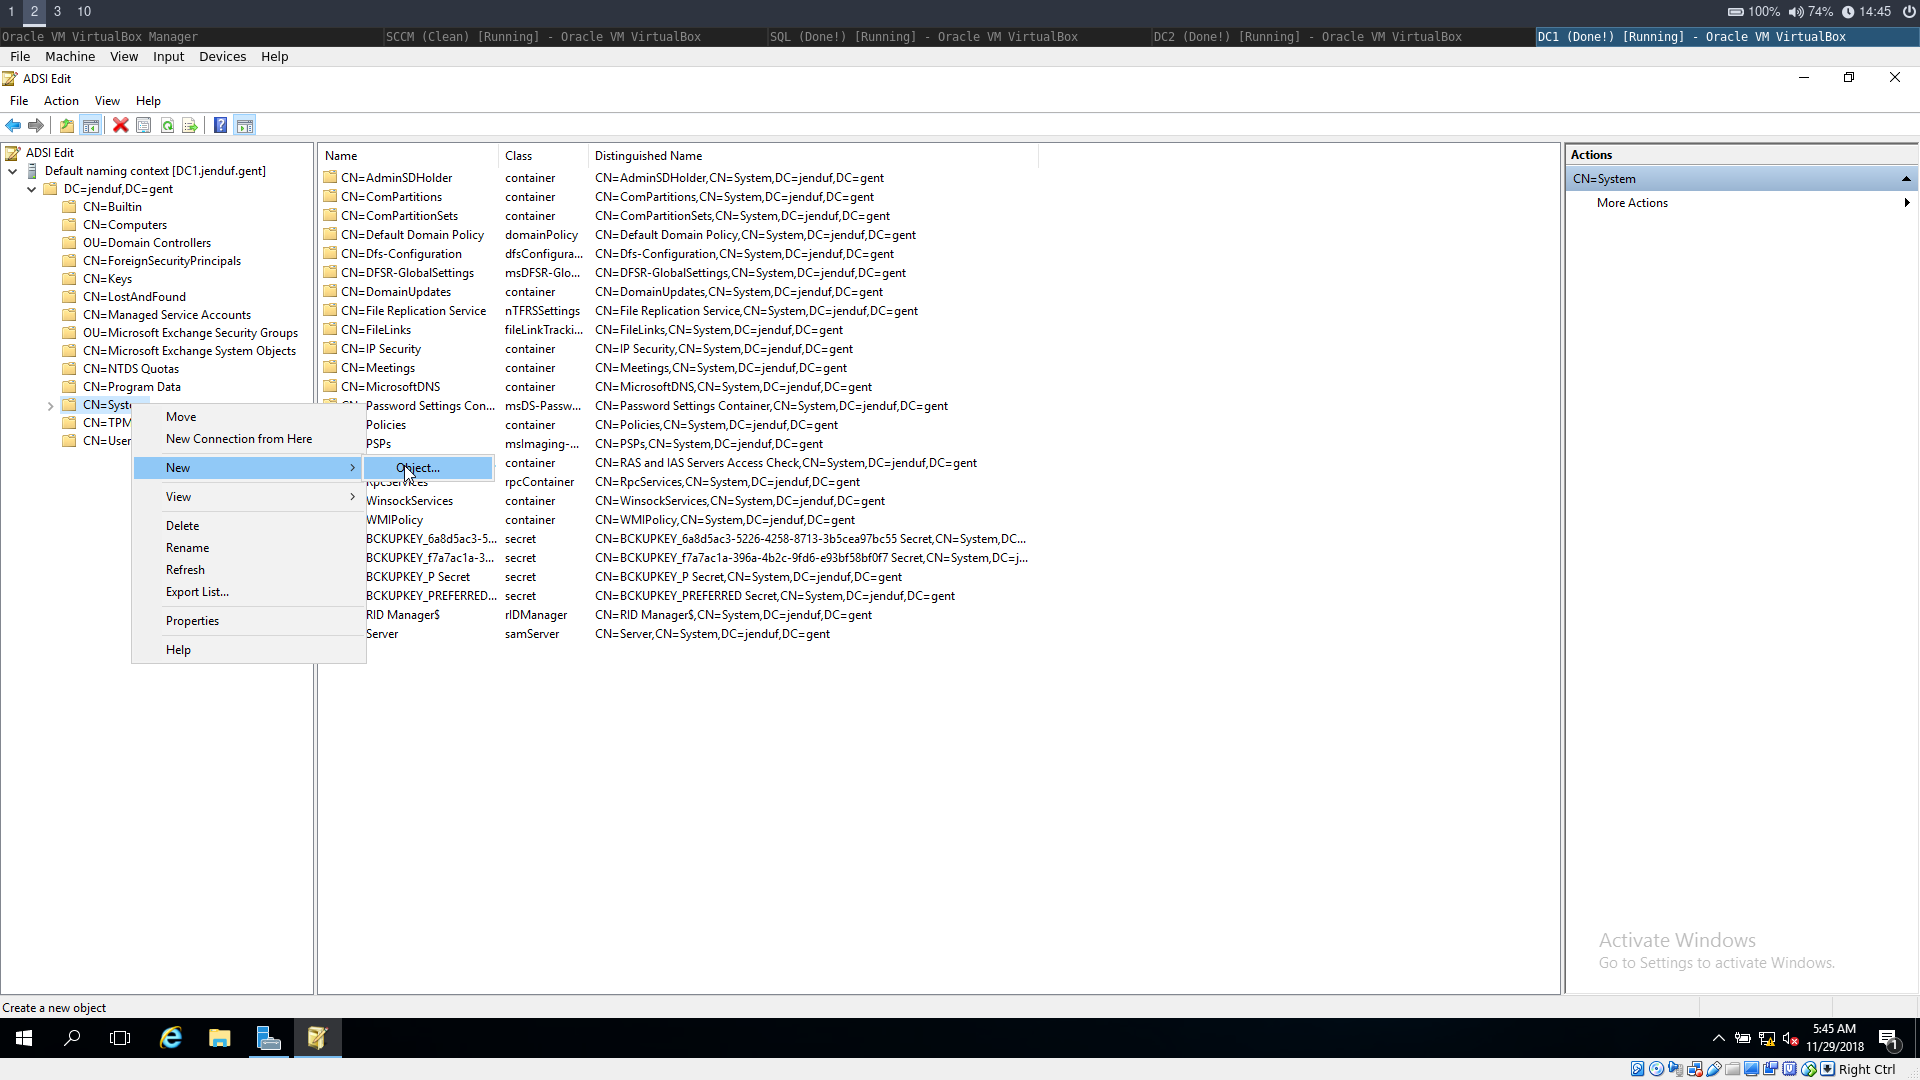
\includegraphics[width=15cm]{Pictures/SCCM/1/1543499145.png}
	
	Maak een nieuw object in "CN=System".
\end{center}
\begin{center}
	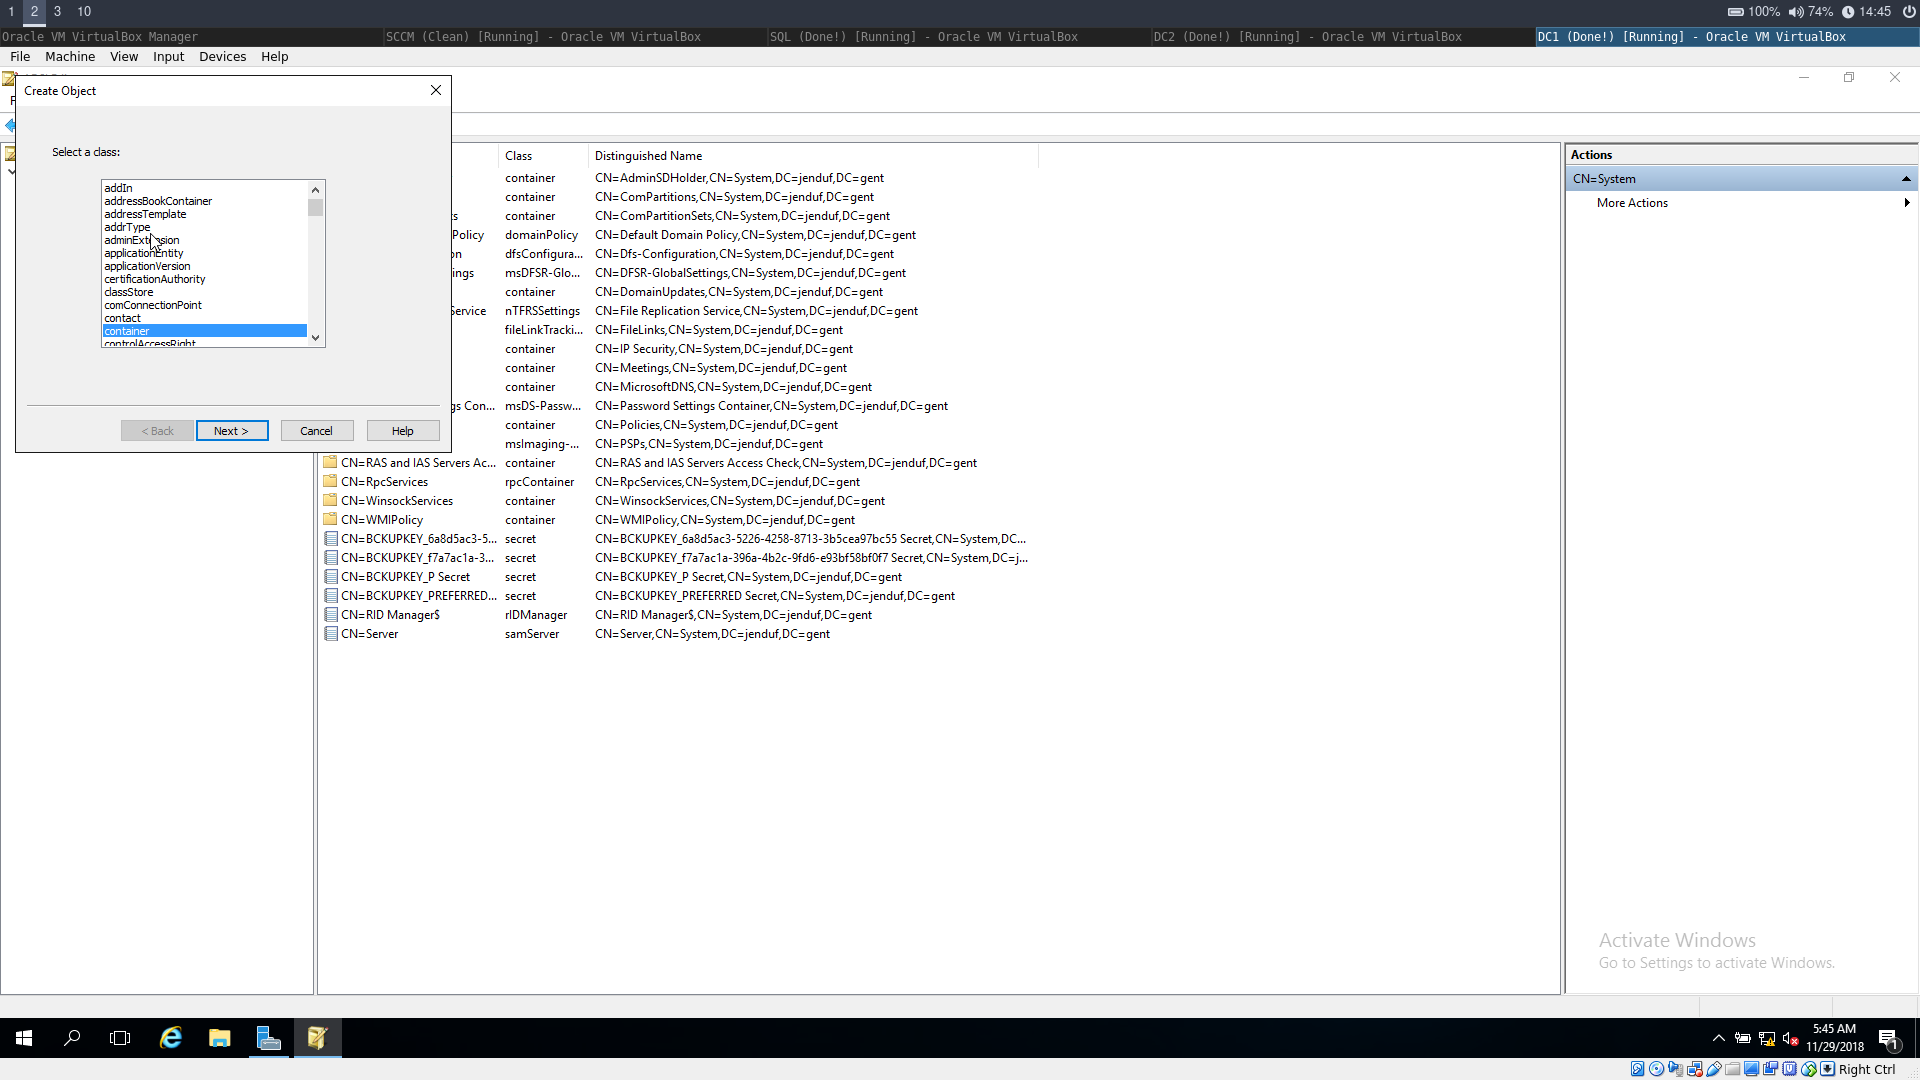
\includegraphics[width=15cm]{Pictures/SCCM/1/1543499150.png}
	Kies de optie "container".
\end{center}
\begin{center}
	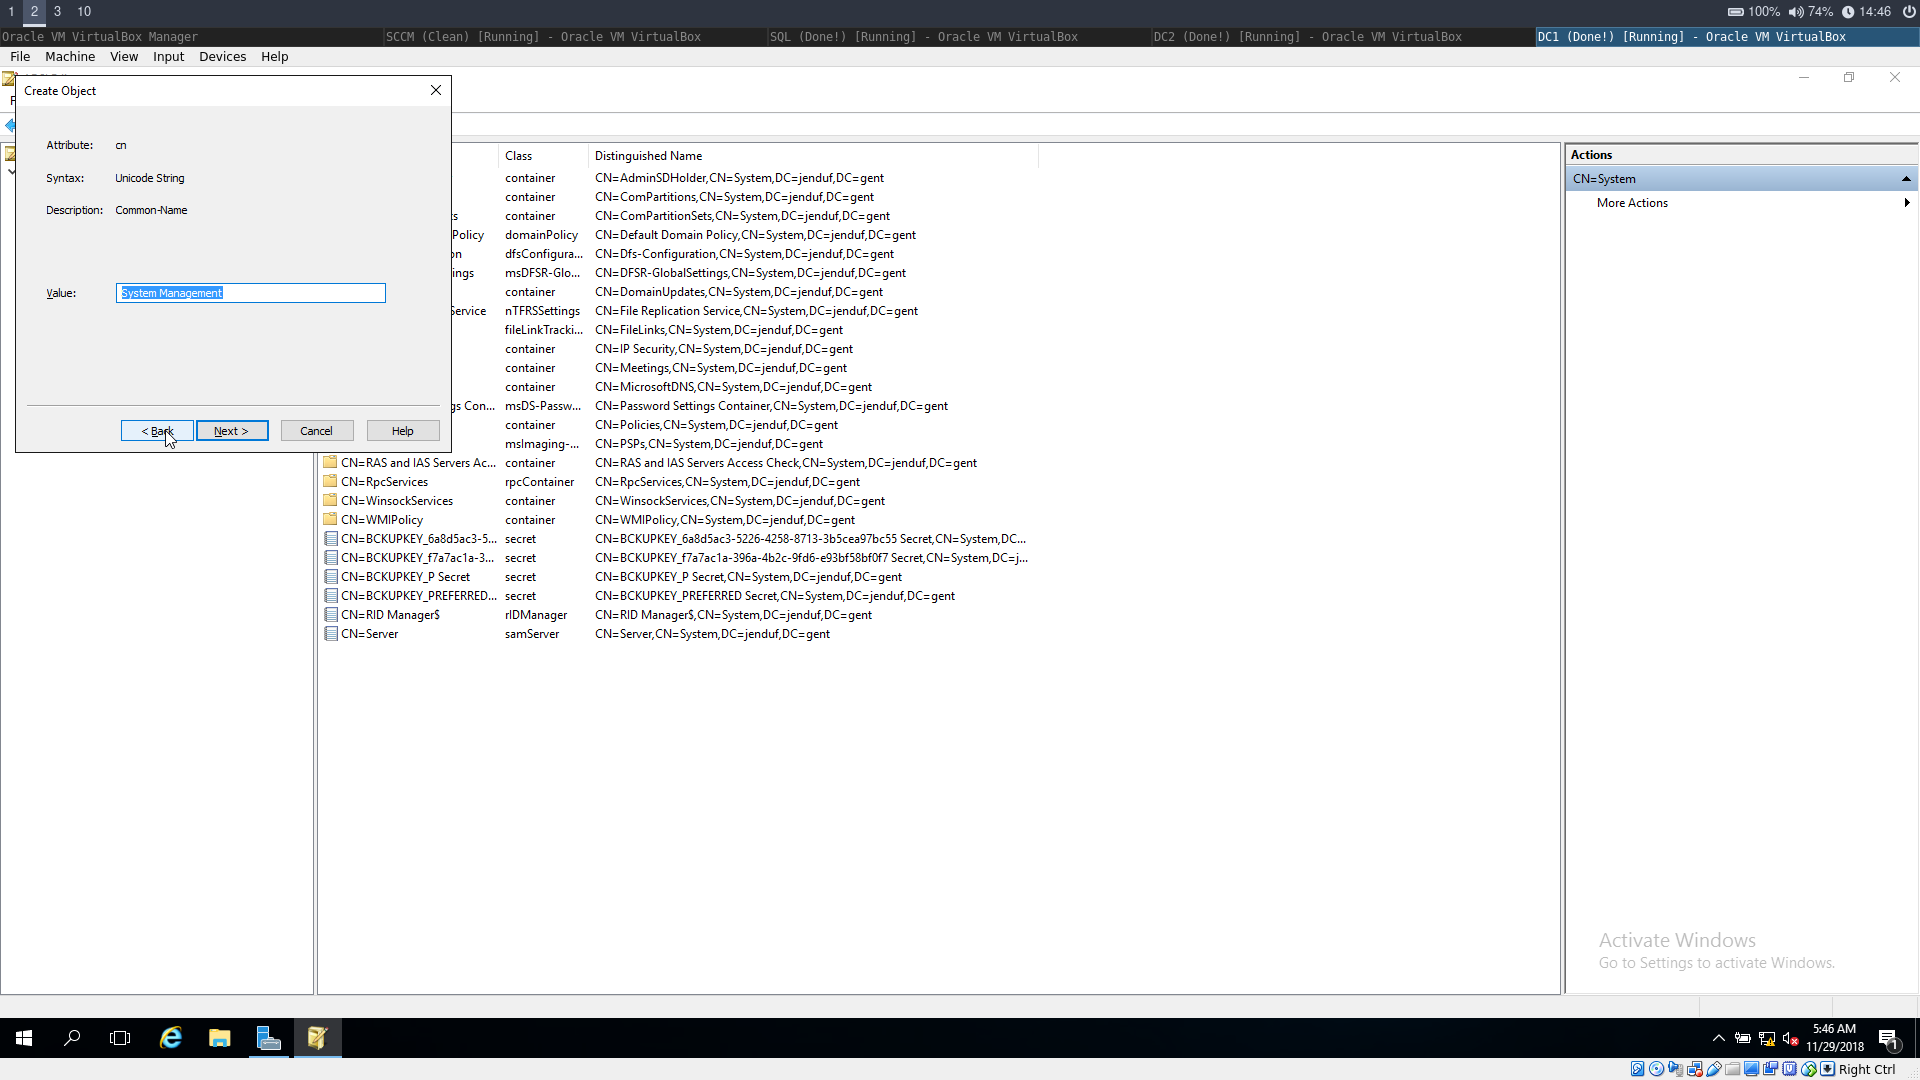
\includegraphics[width=15cm]{Pictures/SCCM/1/1543499210.png}
	
	Geef de container de naam "System Management".
\end{center}
\begin{center}
	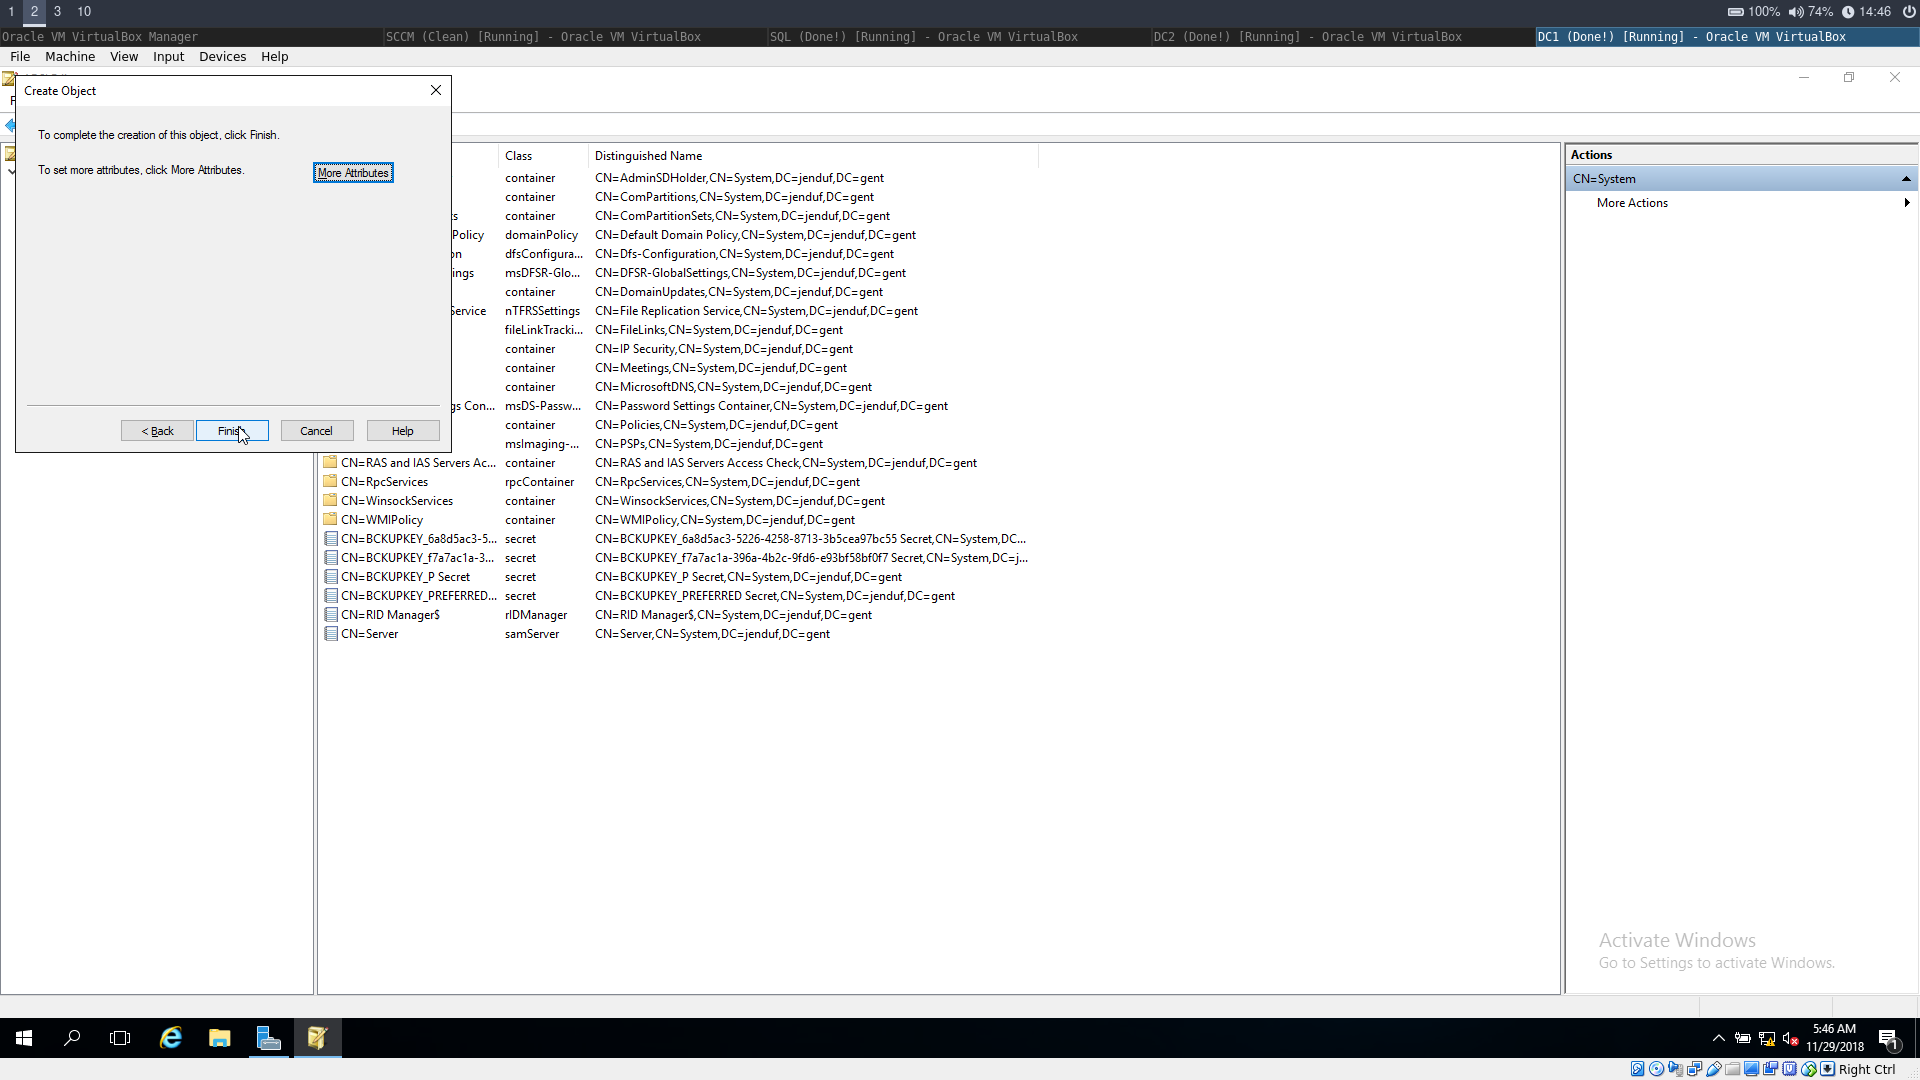
\includegraphics[width=15cm]{Pictures/SCCM/1/1543499213.png}
	
	Klik op "Finish".
\end{center}
\begin{center}
	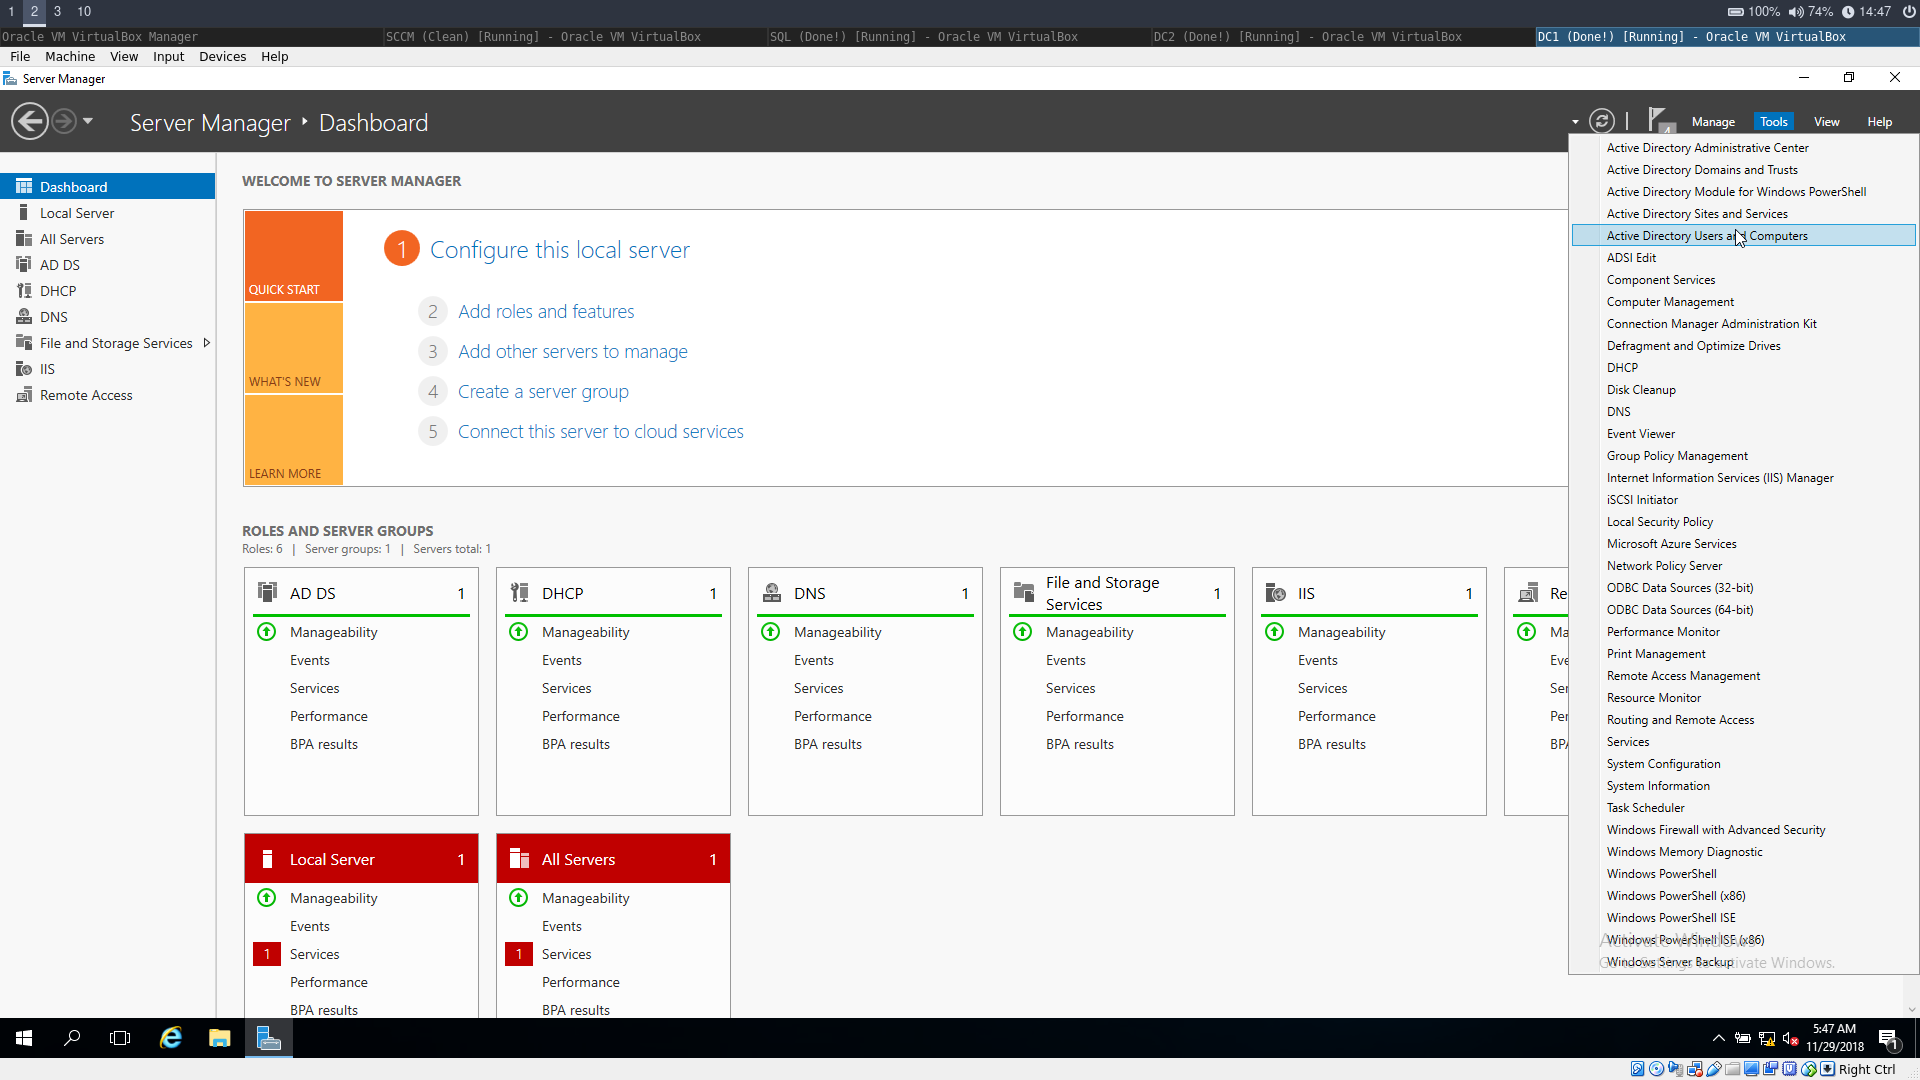
\includegraphics[width=15cm]{Pictures/SCCM/1/1543499275.png}
	
	Open "Active Directory Users and Computers".
\end{center}
\begin{center}
	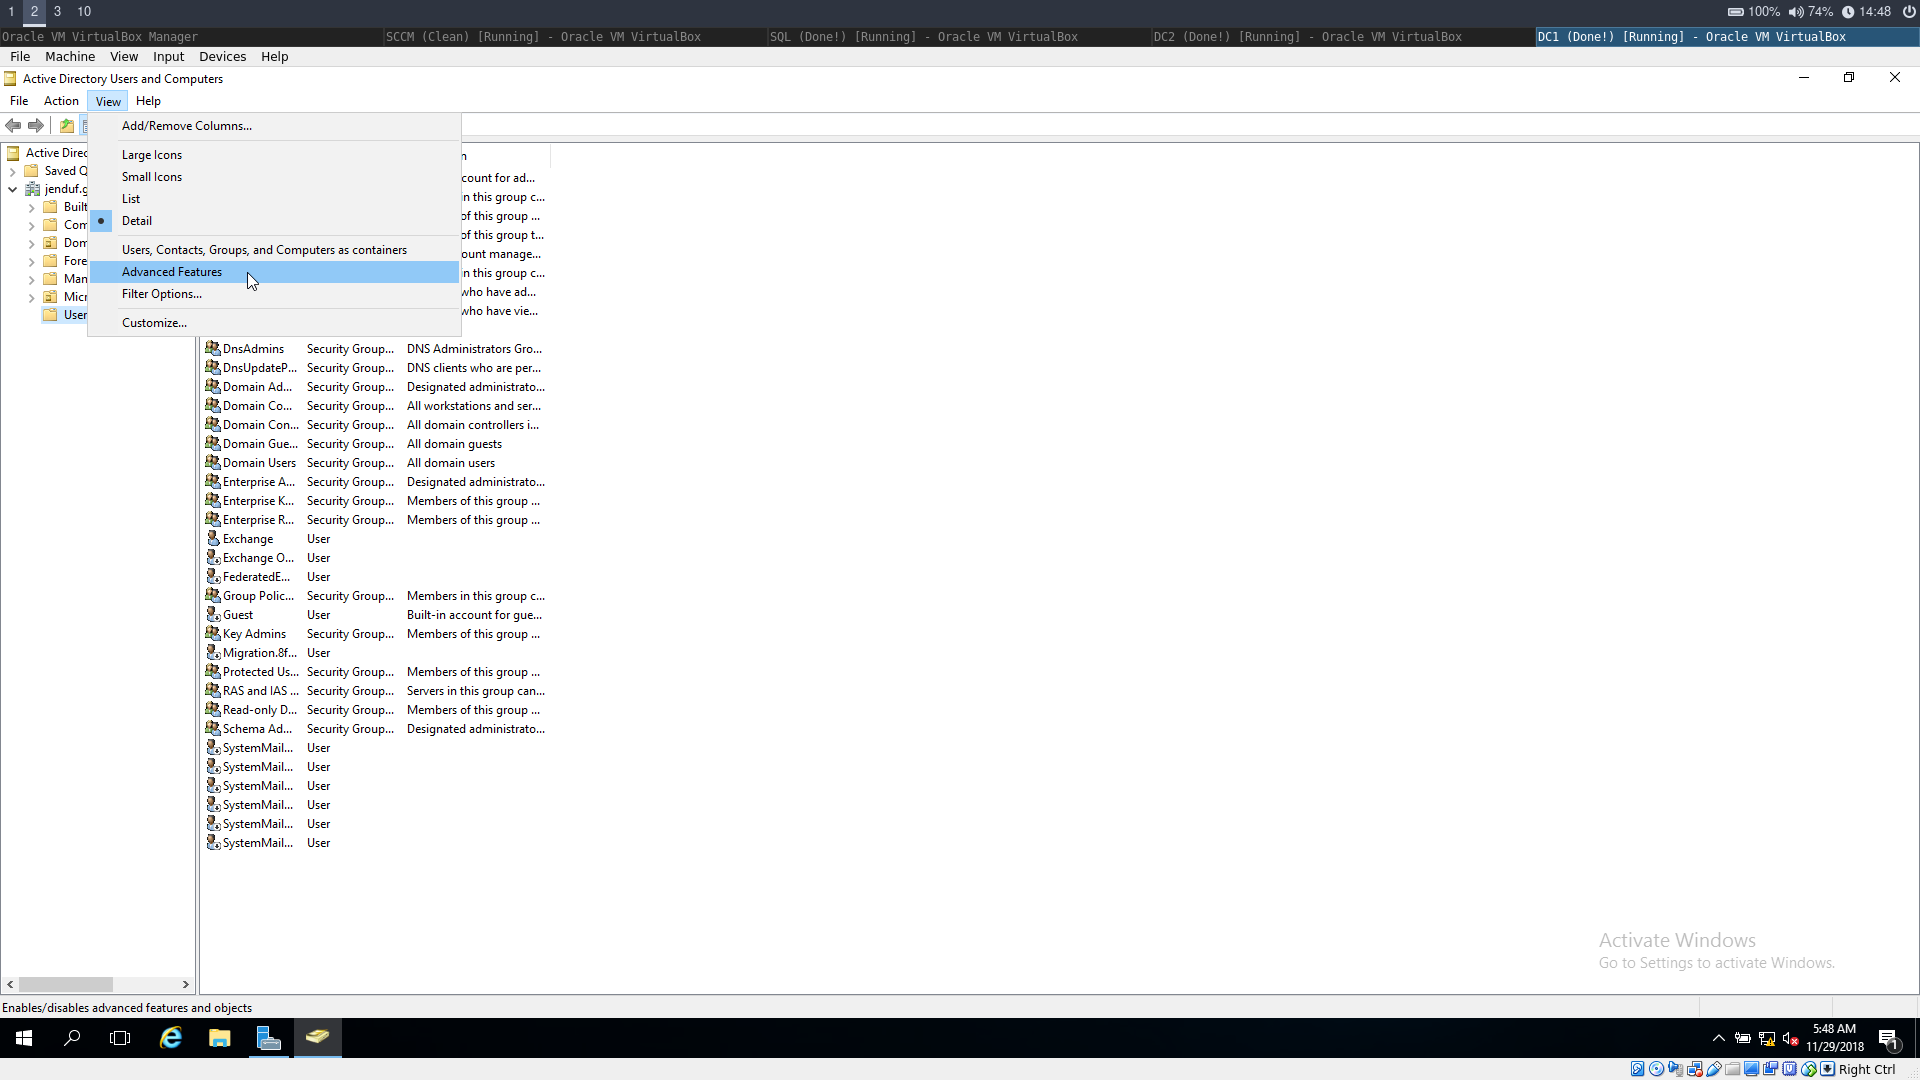
\includegraphics[width=15cm]{Pictures/SCCM/1/1543499288.png}
	
	Toon de "Advanced Features".
\end{center}
\begin{center}
	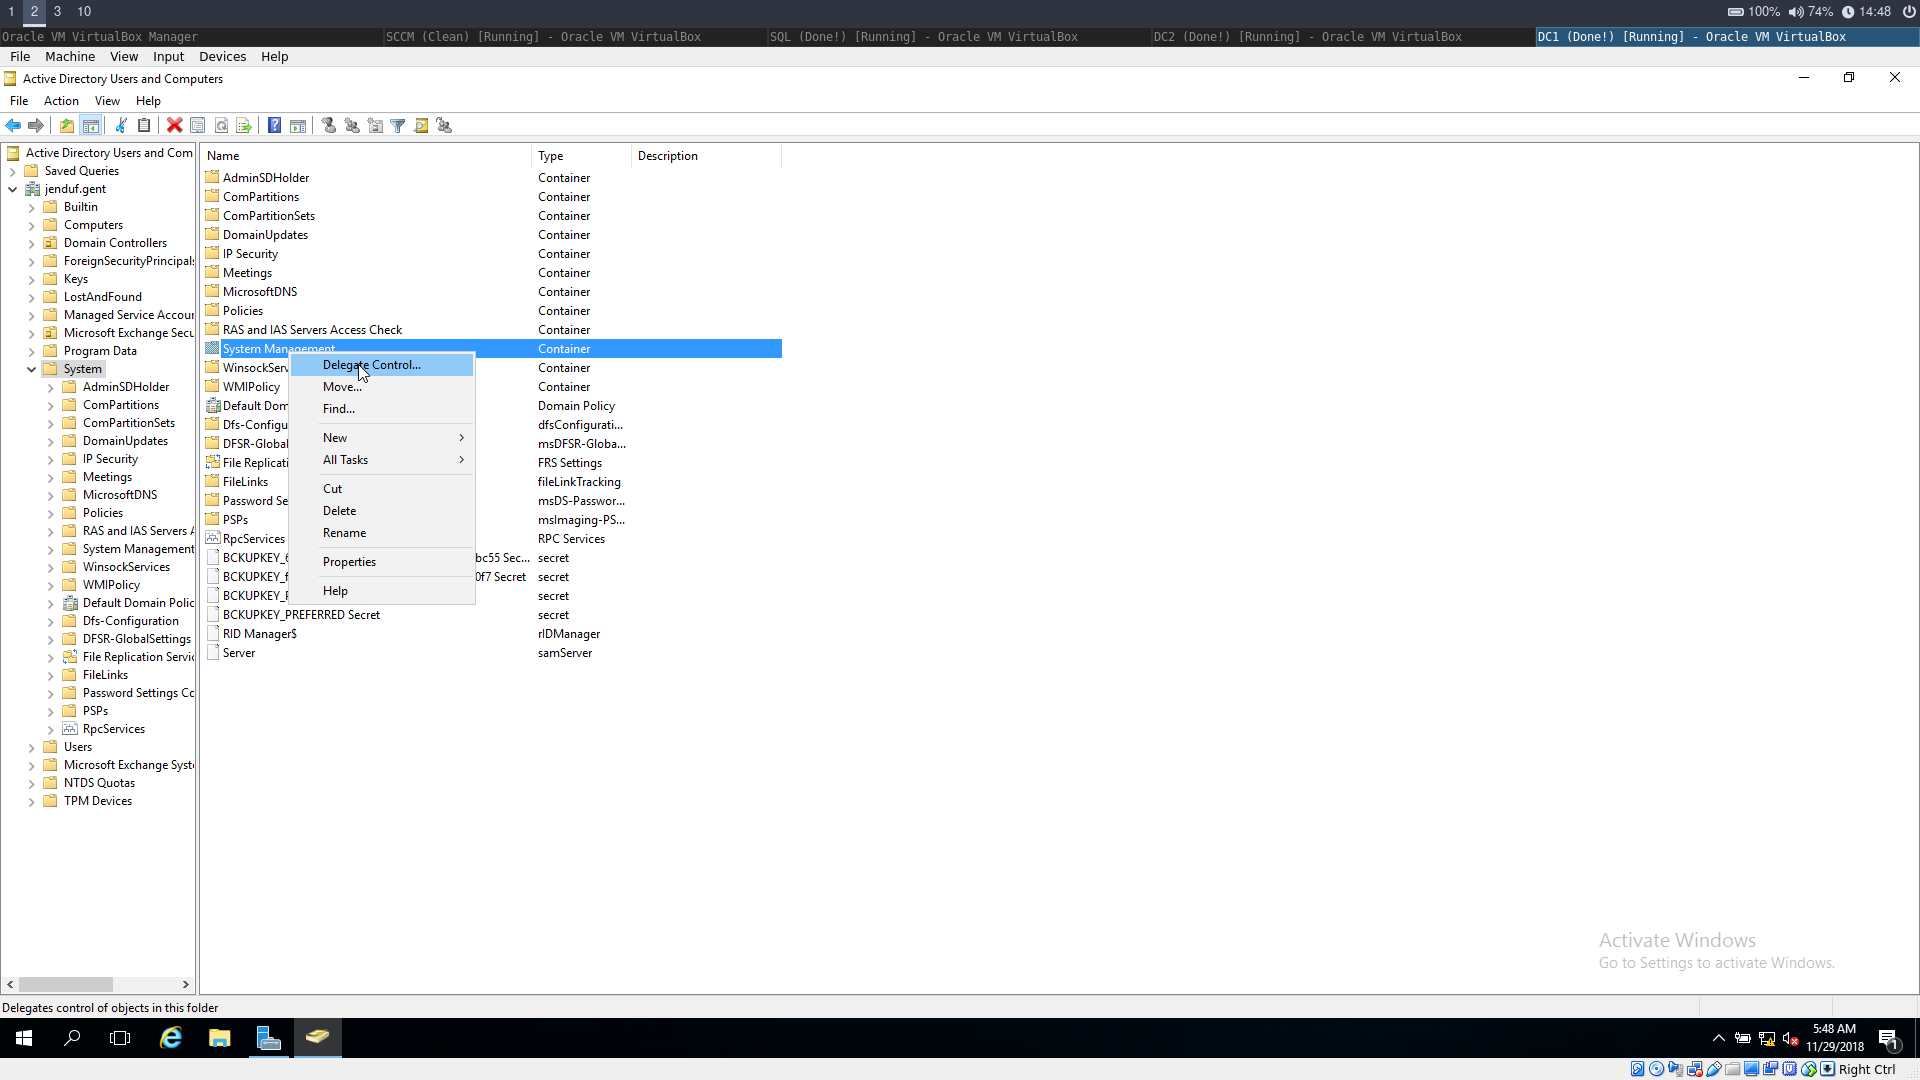
\includegraphics[width=15cm]{Pictures/SCCM/1/1543499299.png}
	
	Klik met de rechtermuisknop op "System Management" en selecteer "Delegate Control".
\end{center}
\begin{center}
	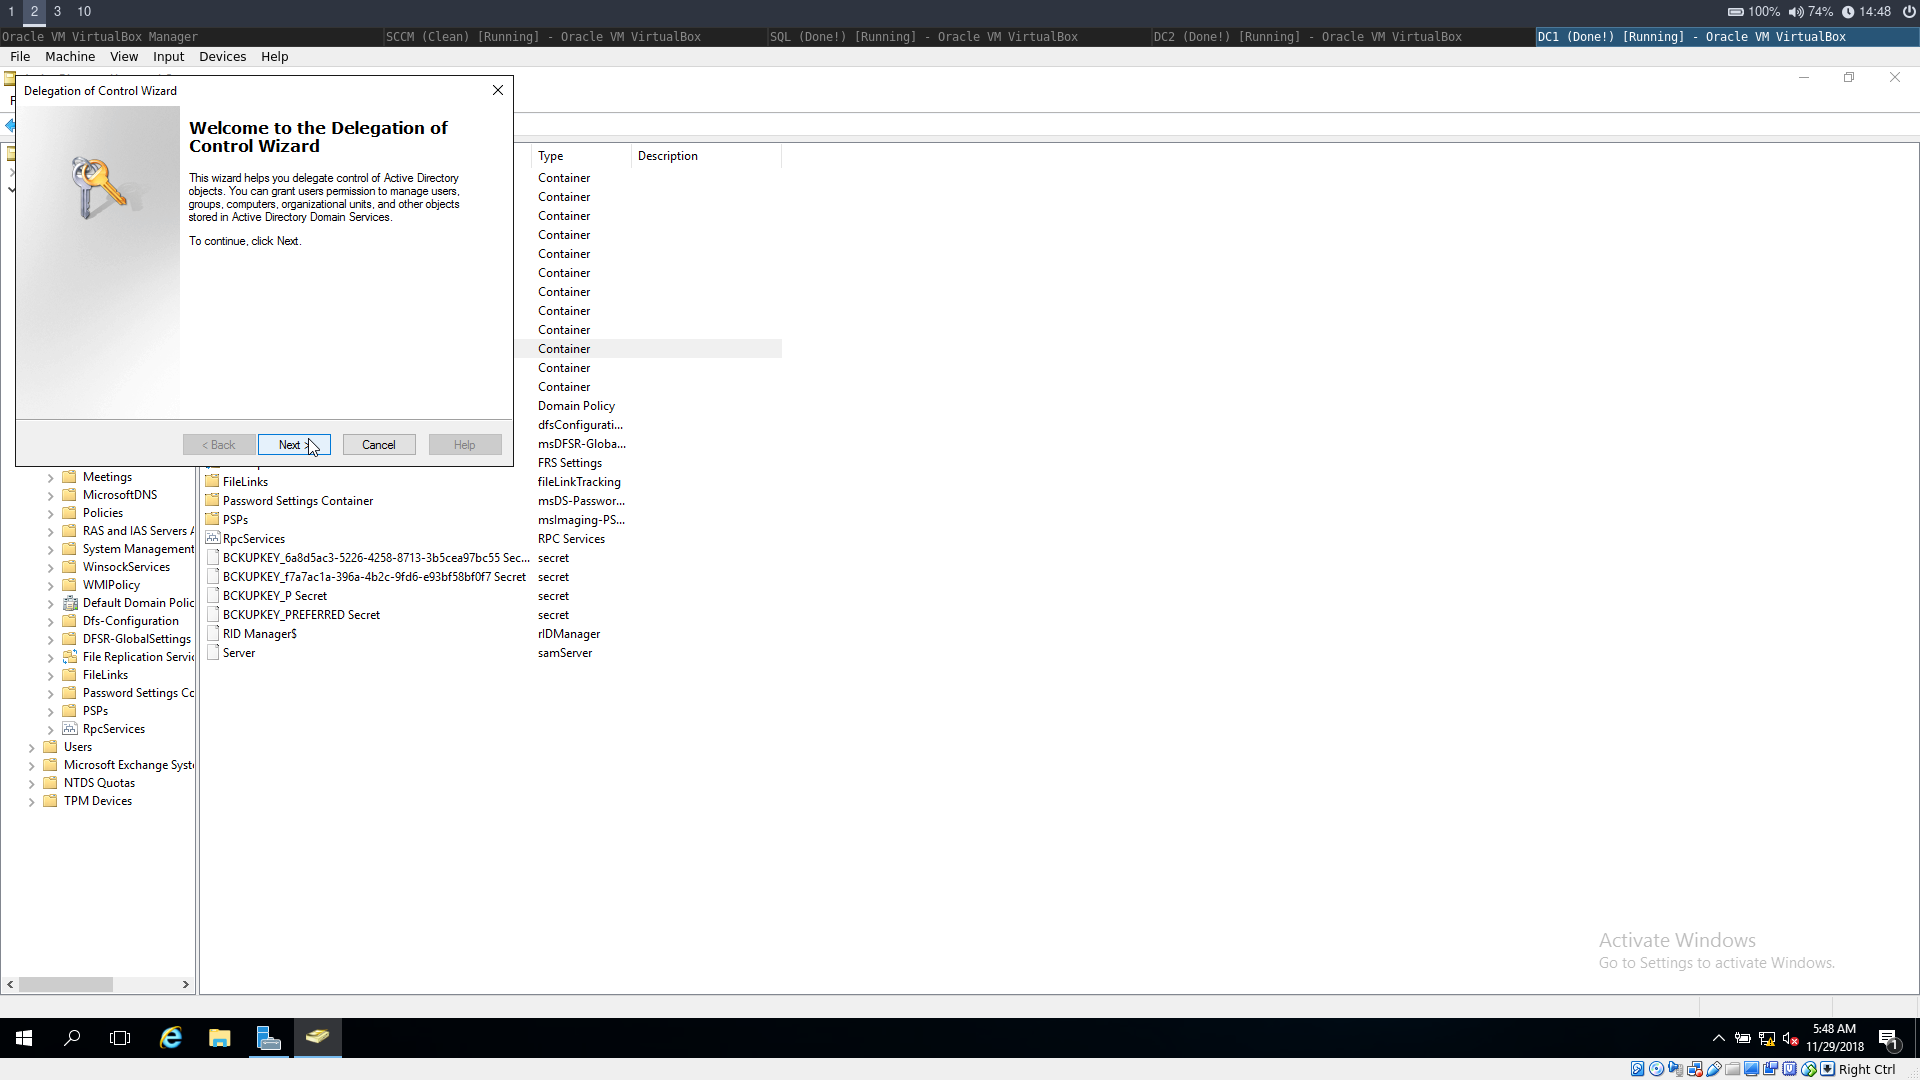
\includegraphics[width=15cm]{Pictures/SCCM/1/1543499303.png}
	
	Klik op "Next".
\end{center}
\begin{center}
	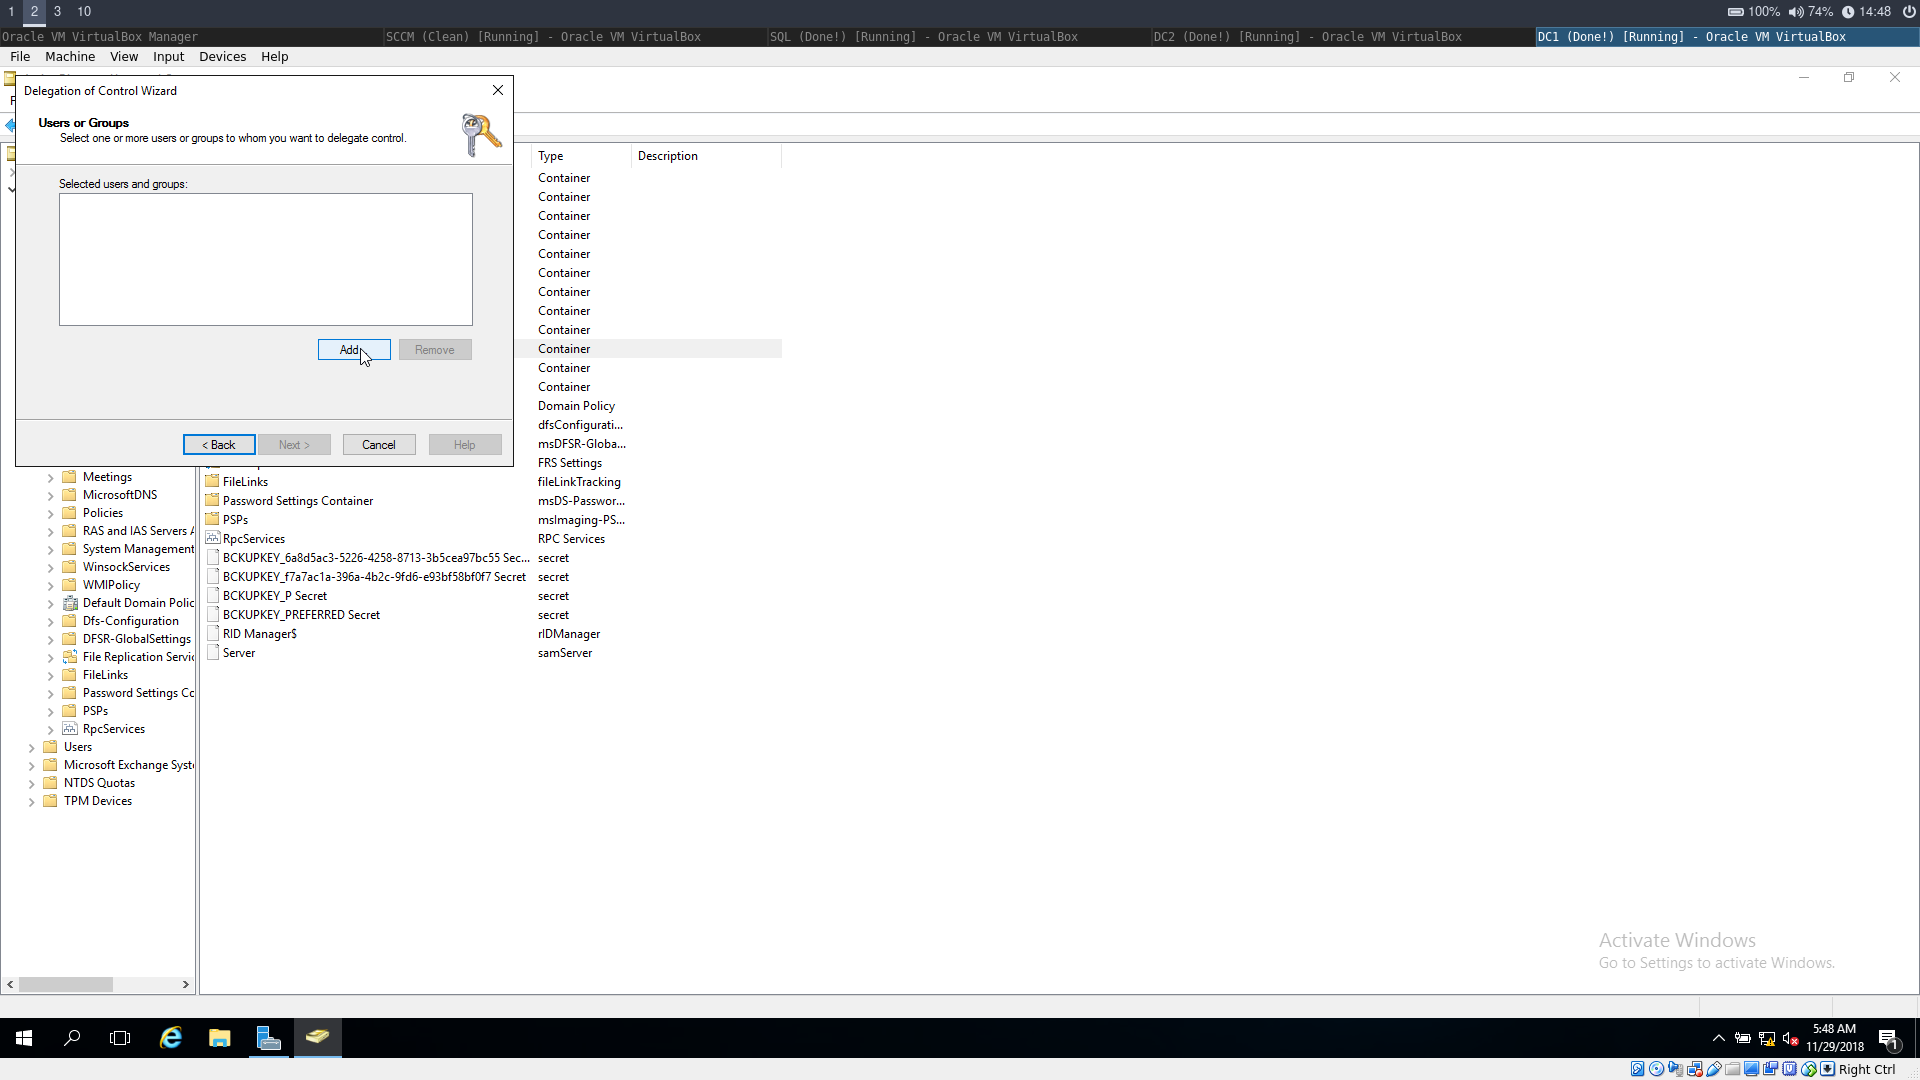
\includegraphics[width=15cm]{Pictures/SCCM/1/1543499309.png}
	
	Klik op "Add".
\end{center}
\begin{center}
	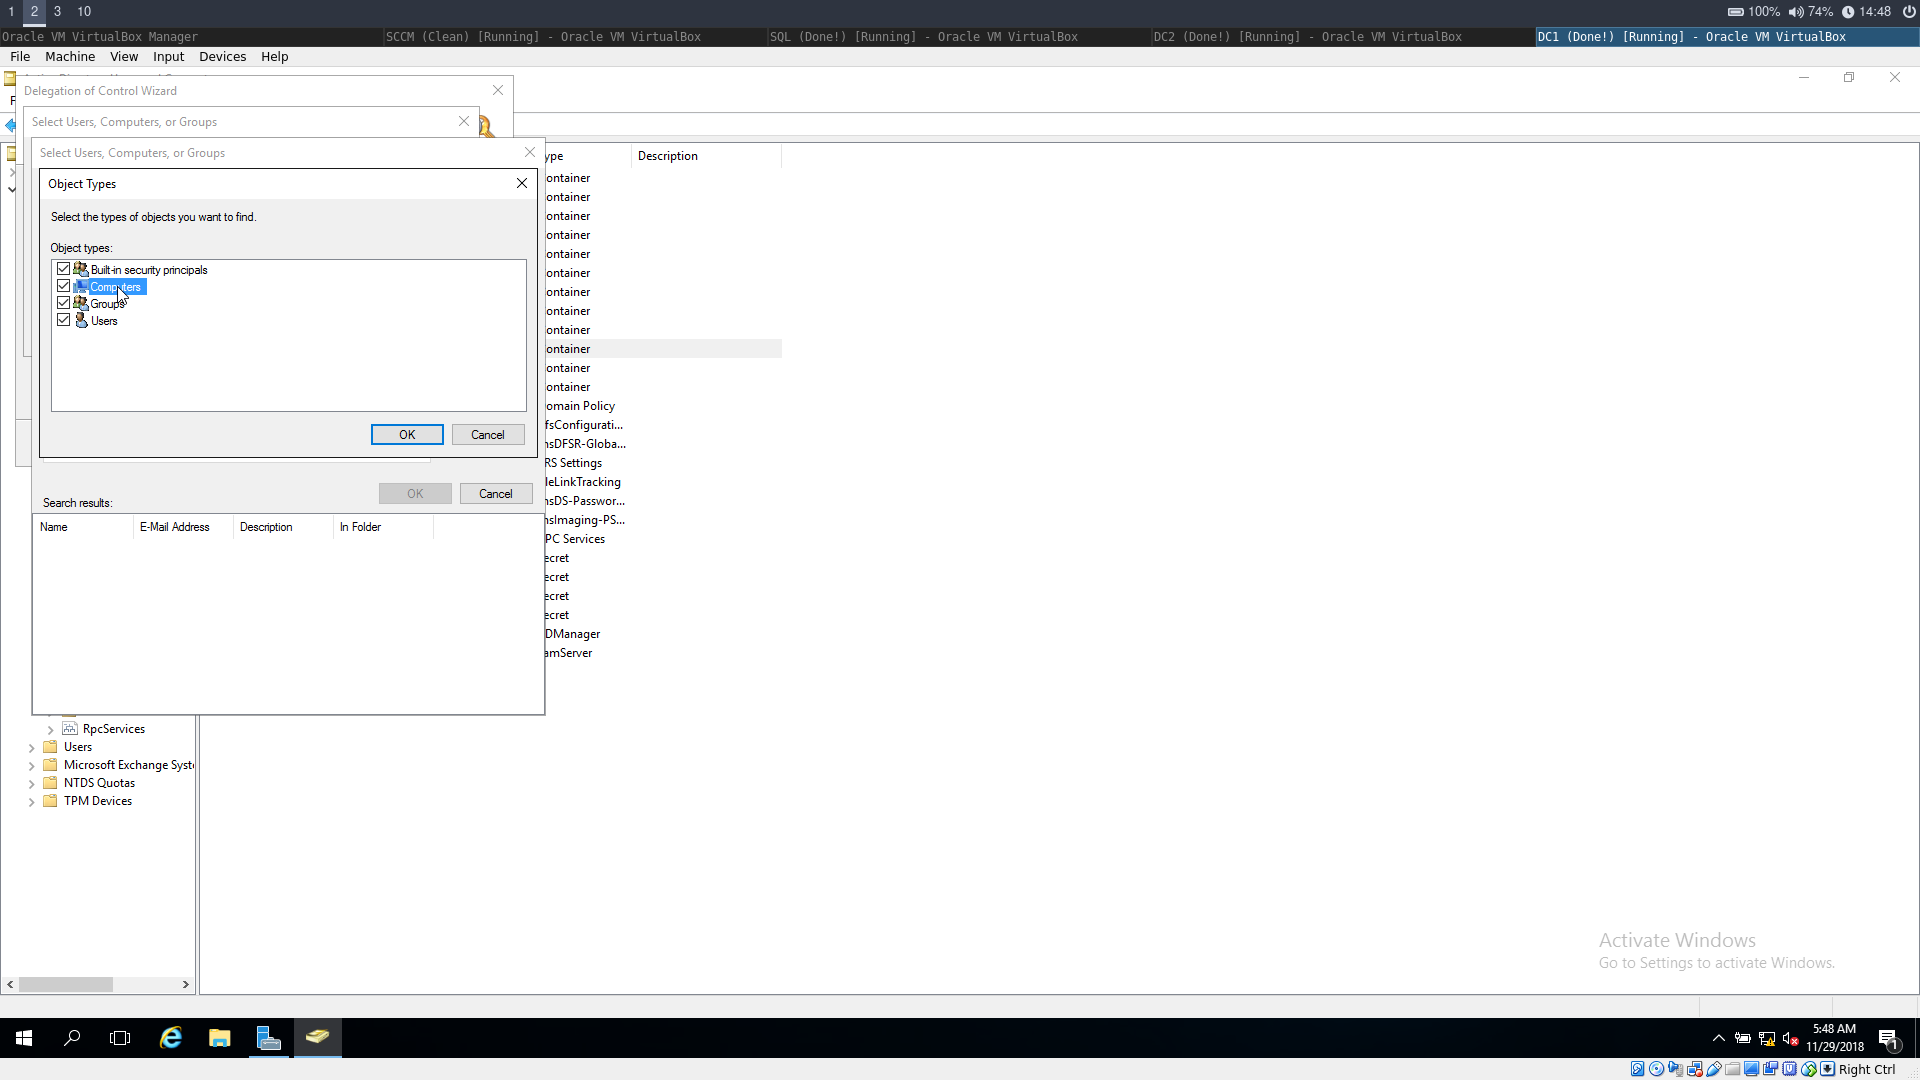
\includegraphics[width=15cm]{Pictures/SCCM/1/1543499322.png}
	
	Vink "Computers" aan in de geselecteerde "Object Types".
\end{center}
\begin{center}
	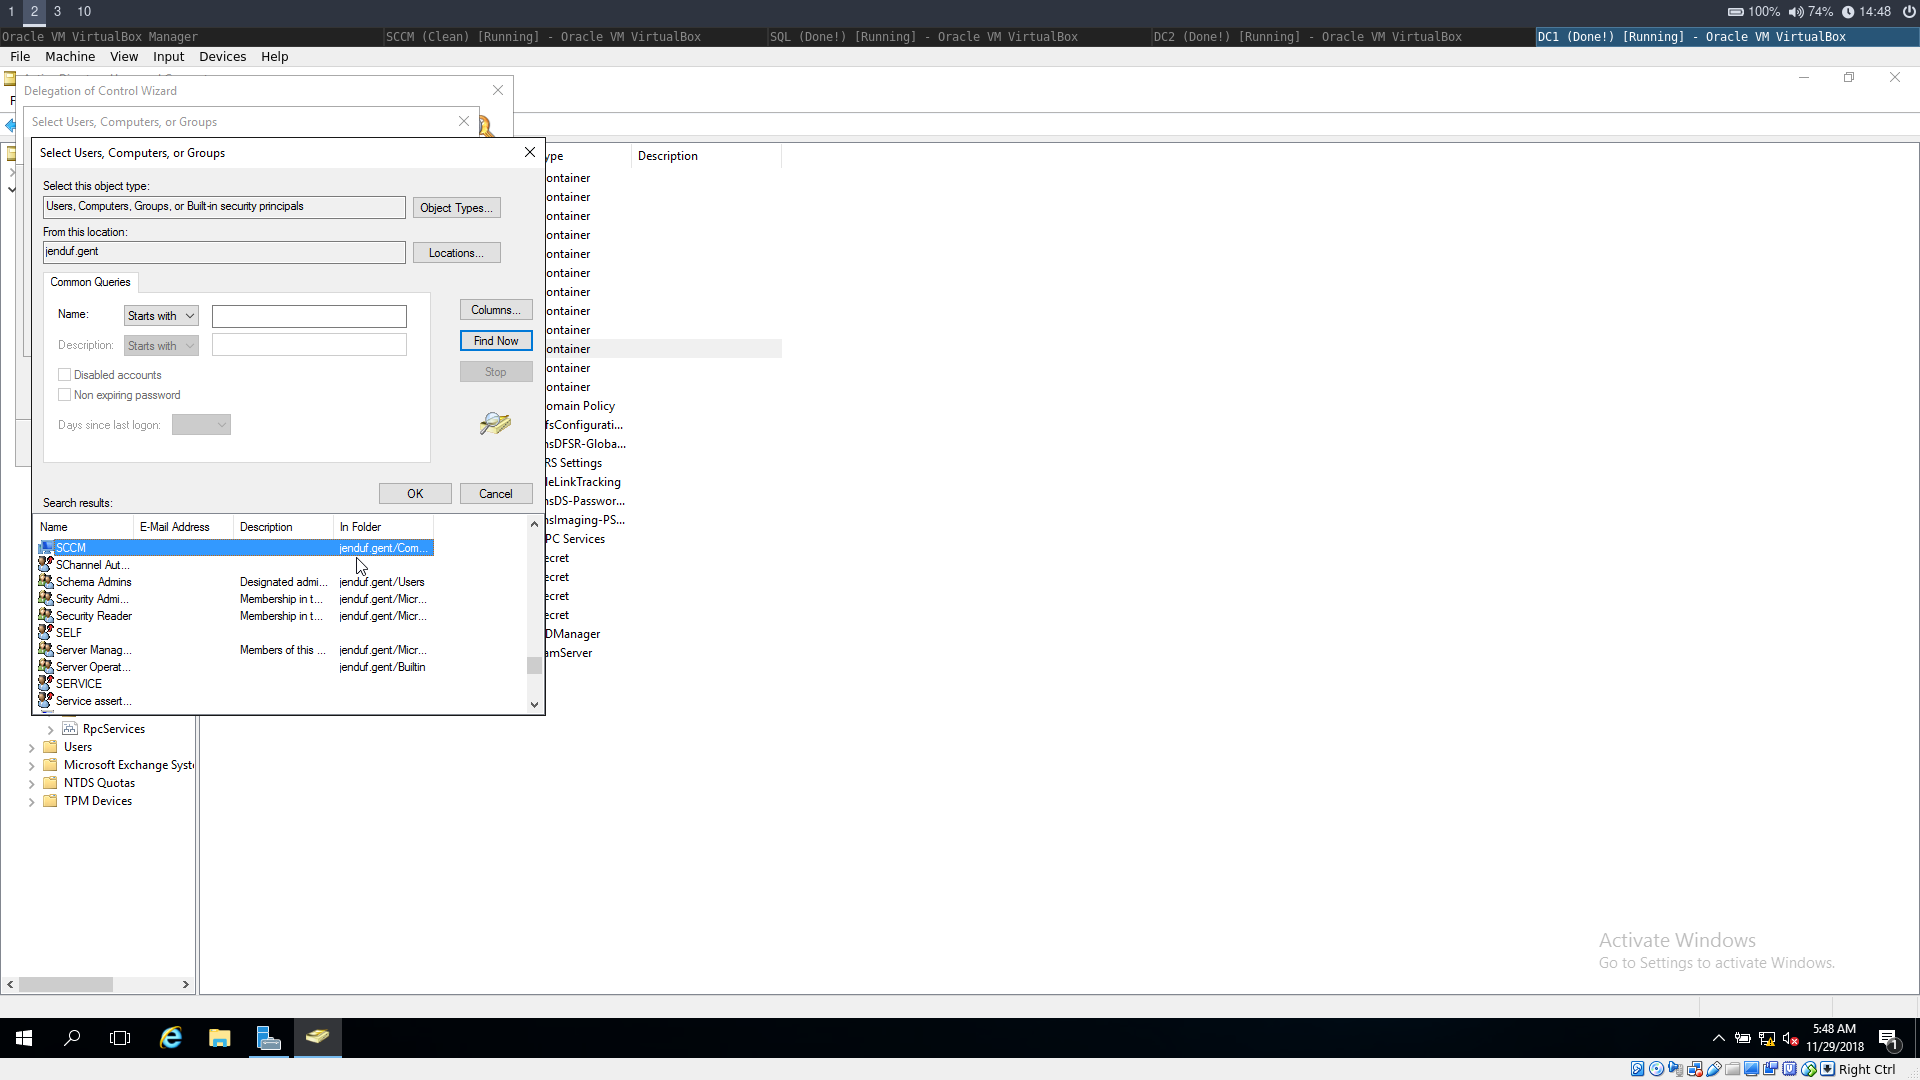
\includegraphics[width=15cm]{Pictures/SCCM/1/1543499331.png}
	
	Selecteer de computer "SCCM".
\end{center}
\begin{center}
	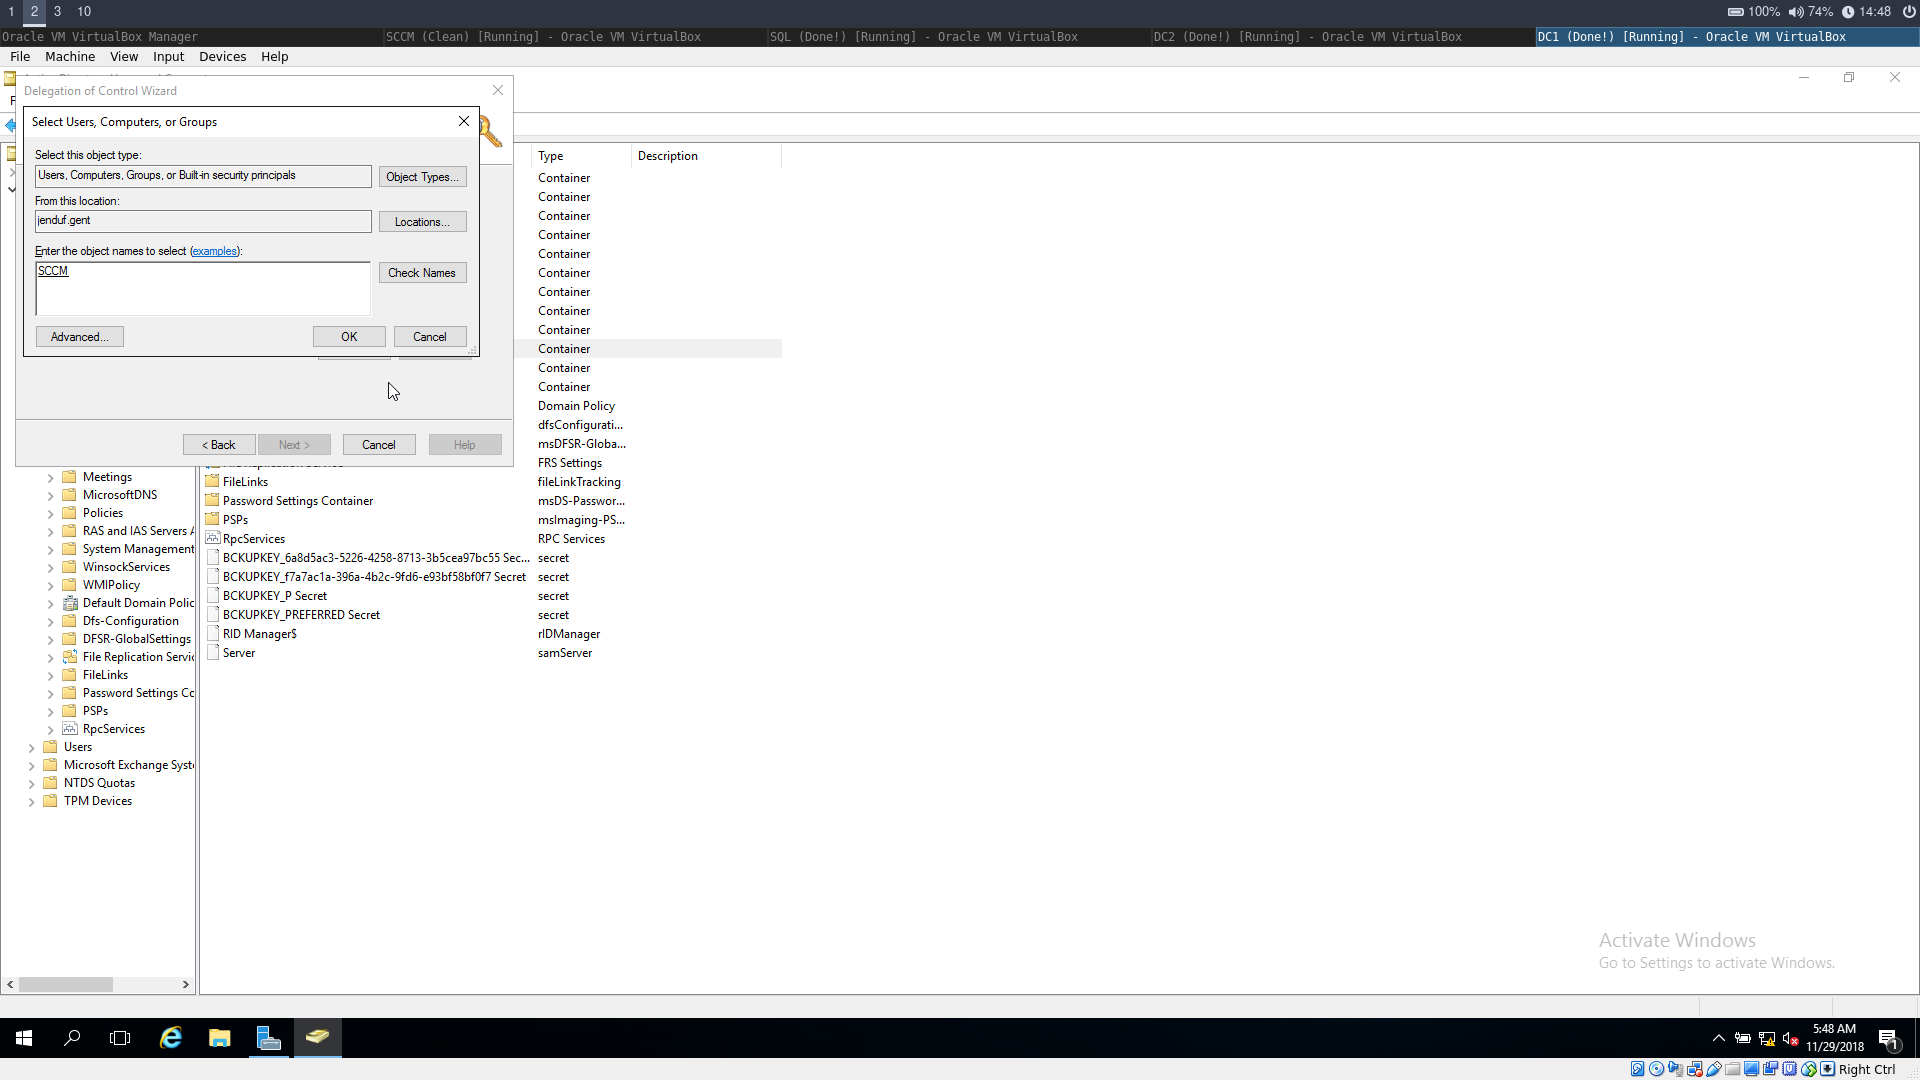
\includegraphics[width=15cm]{Pictures/SCCM/1/1543499333.png}


\end{center}
\begin{center}
	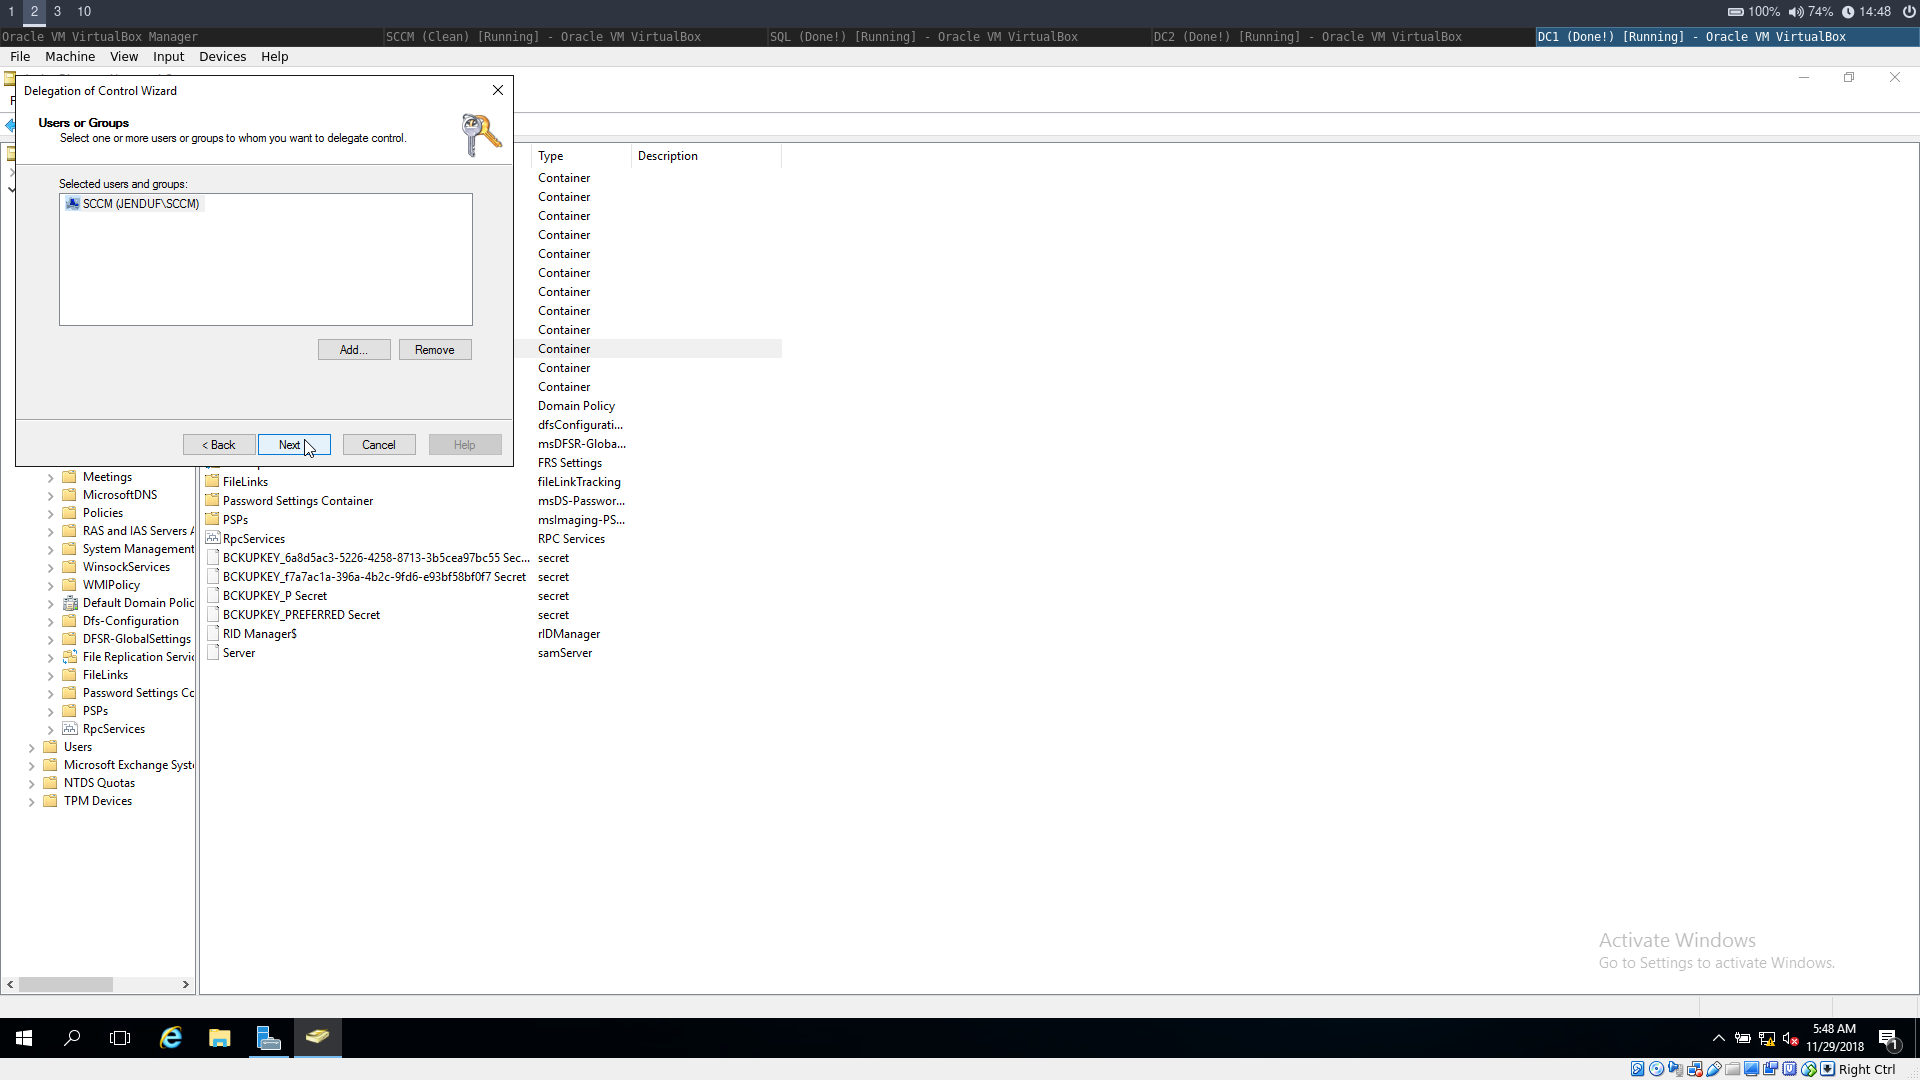
\includegraphics[width=15cm]{Pictures/SCCM/1/1543499336.png}
	
	Ga verder met configuratiewizard.
\end{center}
\begin{center}
	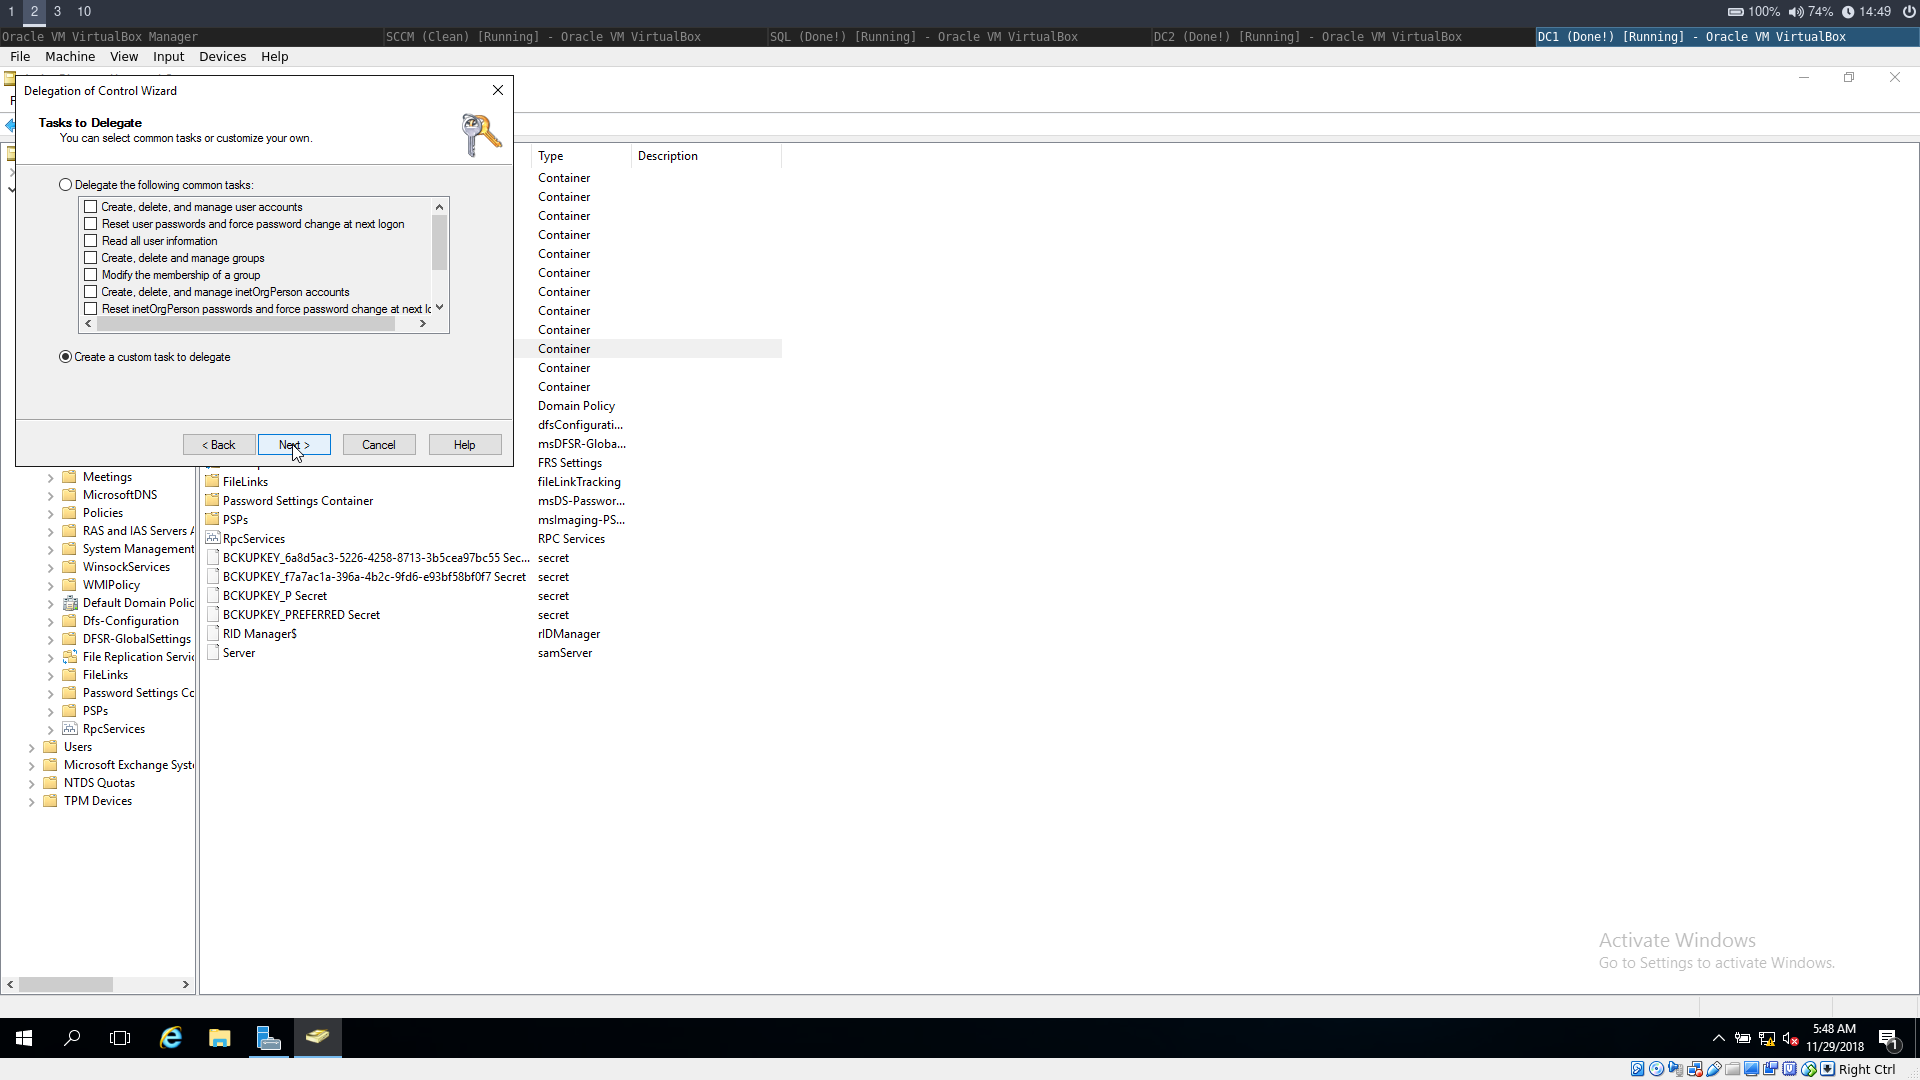
\includegraphics[width=15cm]{Pictures/SCCM/1/1543499340.png}
	
	Selecteer "Create a costum task to delegate".
\end{center}
\begin{center}
	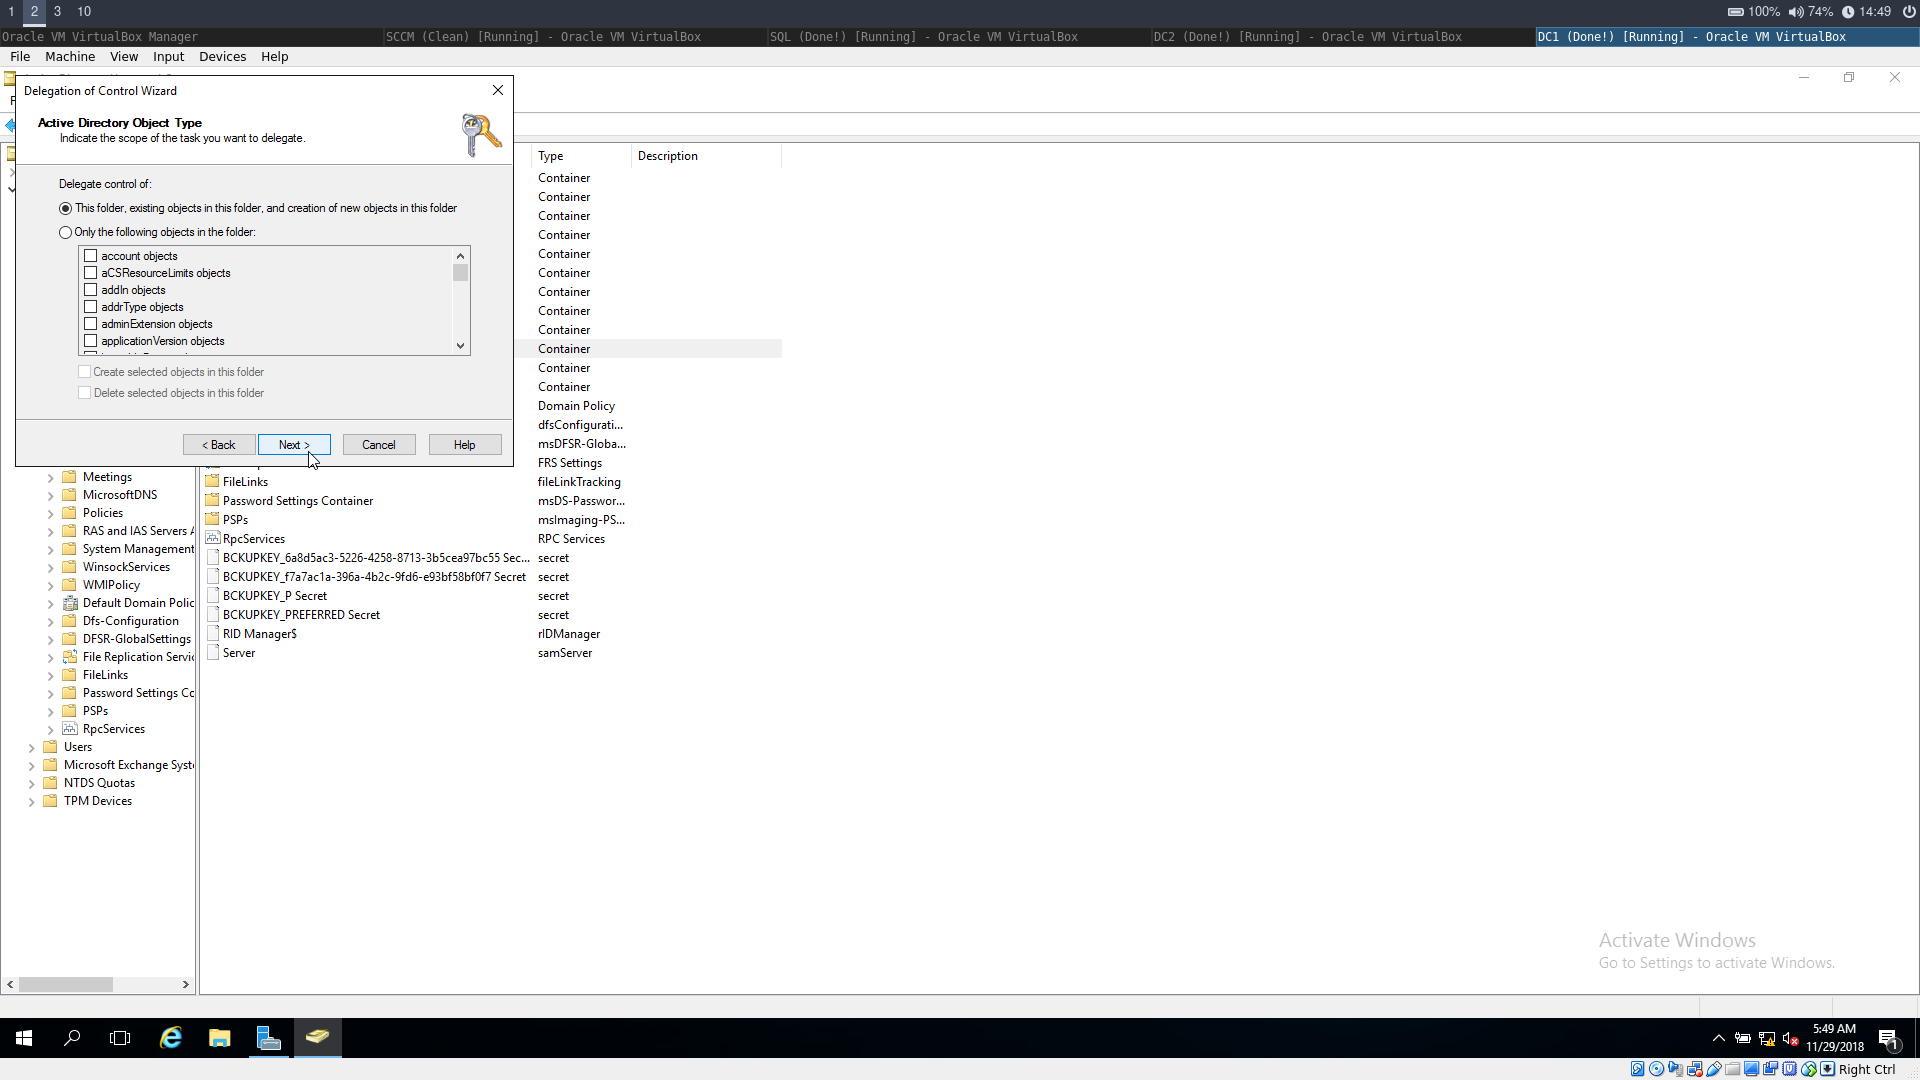
\includegraphics[width=15cm]{Pictures/SCCM/1/1543499344.png}
	
	Klik op volgende.
\end{center}
\begin{center}
	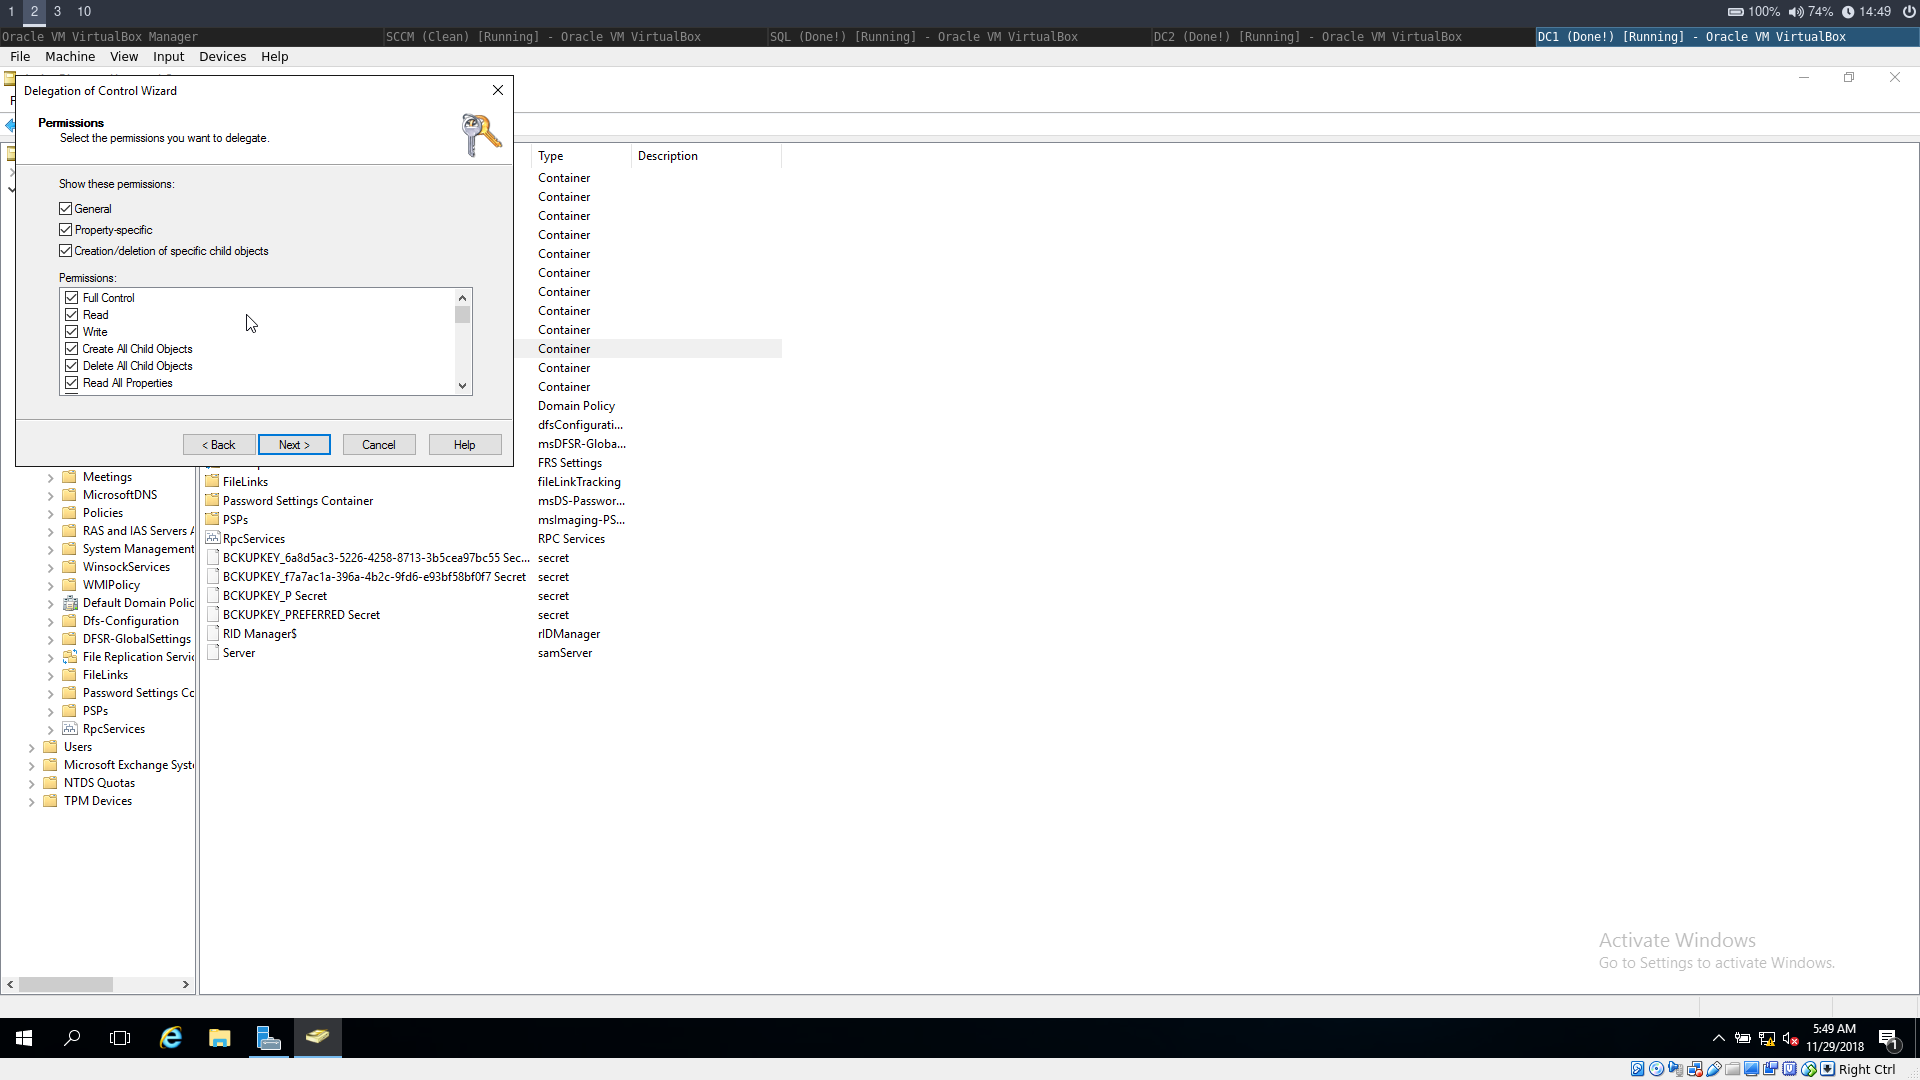
\includegraphics[width=15cm]{Pictures/SCCM/1/1543499353.png}
	
		Vink alle bovenstaande opties aan en selecteer "Full Control".

\end{center}
\begin{center}
	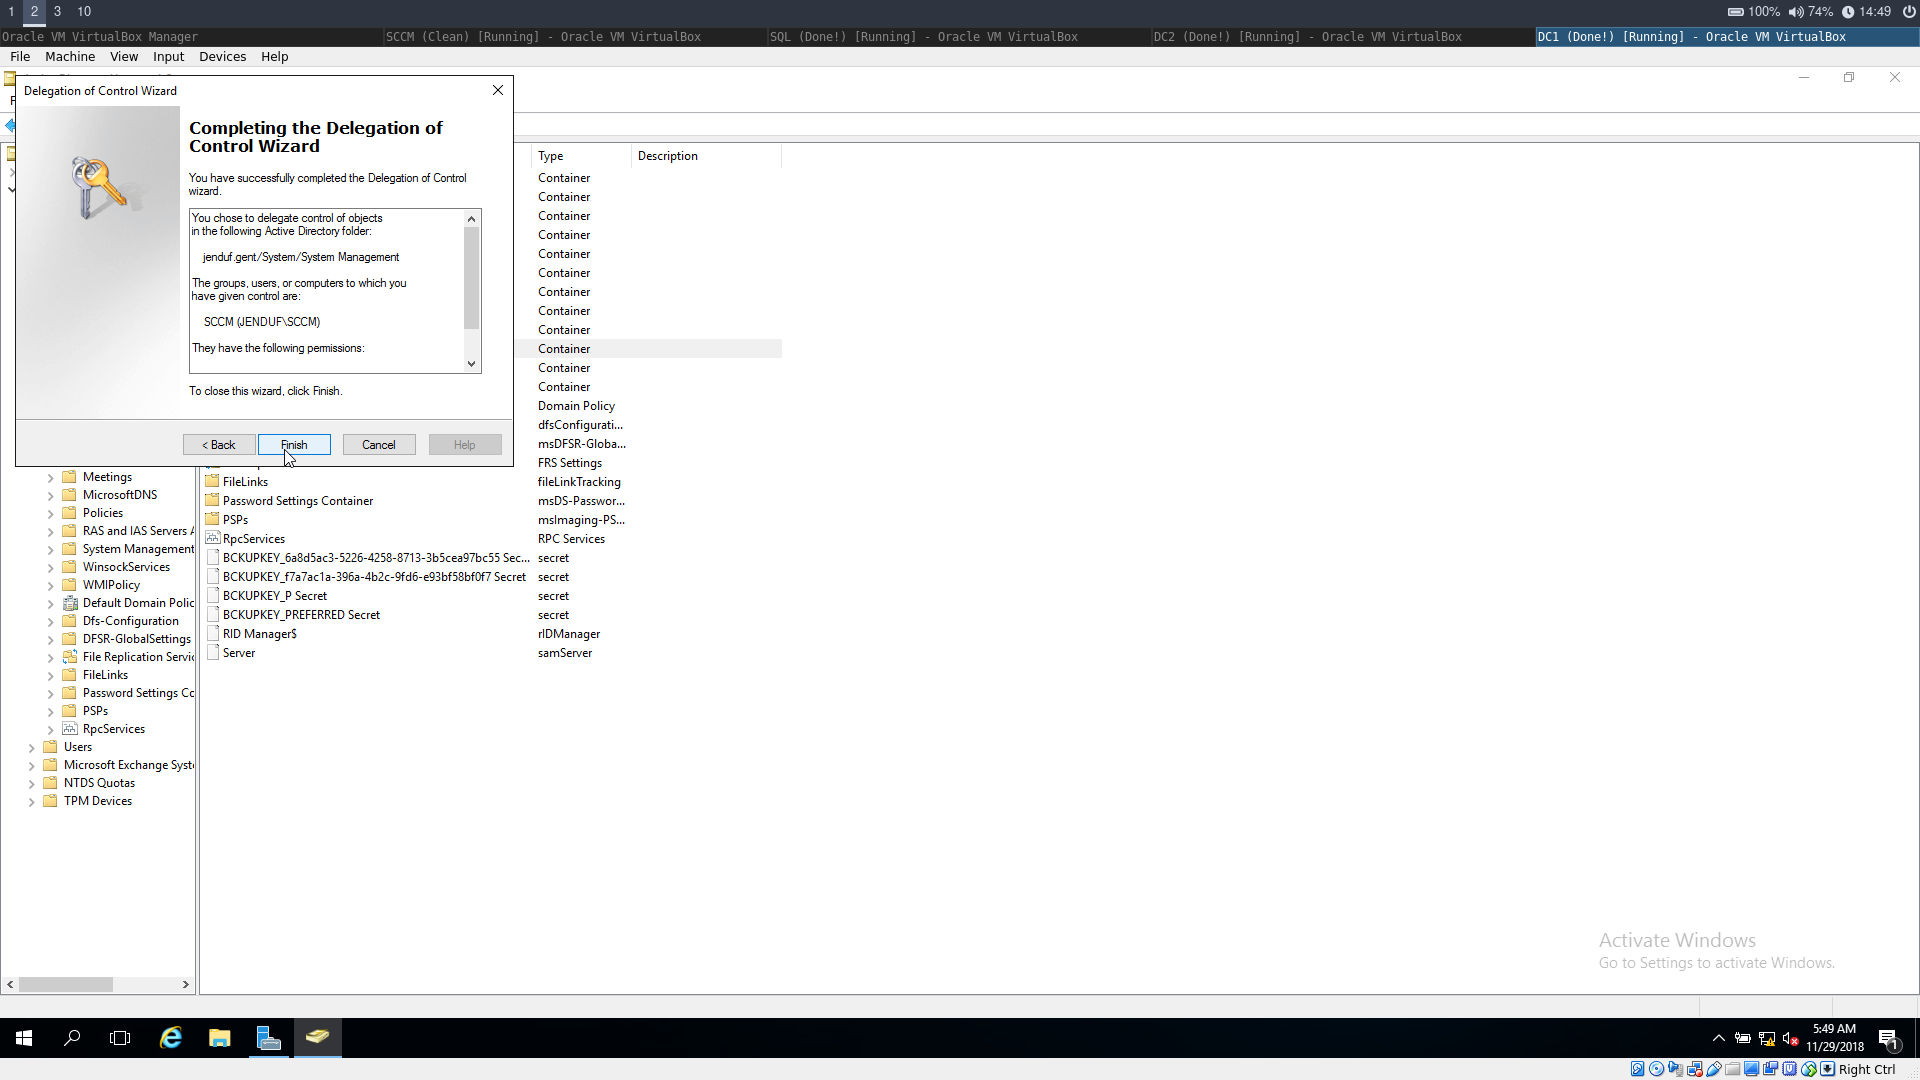
\includegraphics[width=15cm]{Pictures/SCCM/1/1543499355.png}
	
		Voltooi de configuratiewizard.
\end{center}
\subsection{Extending Active Directory Schema}
\begin{center}
	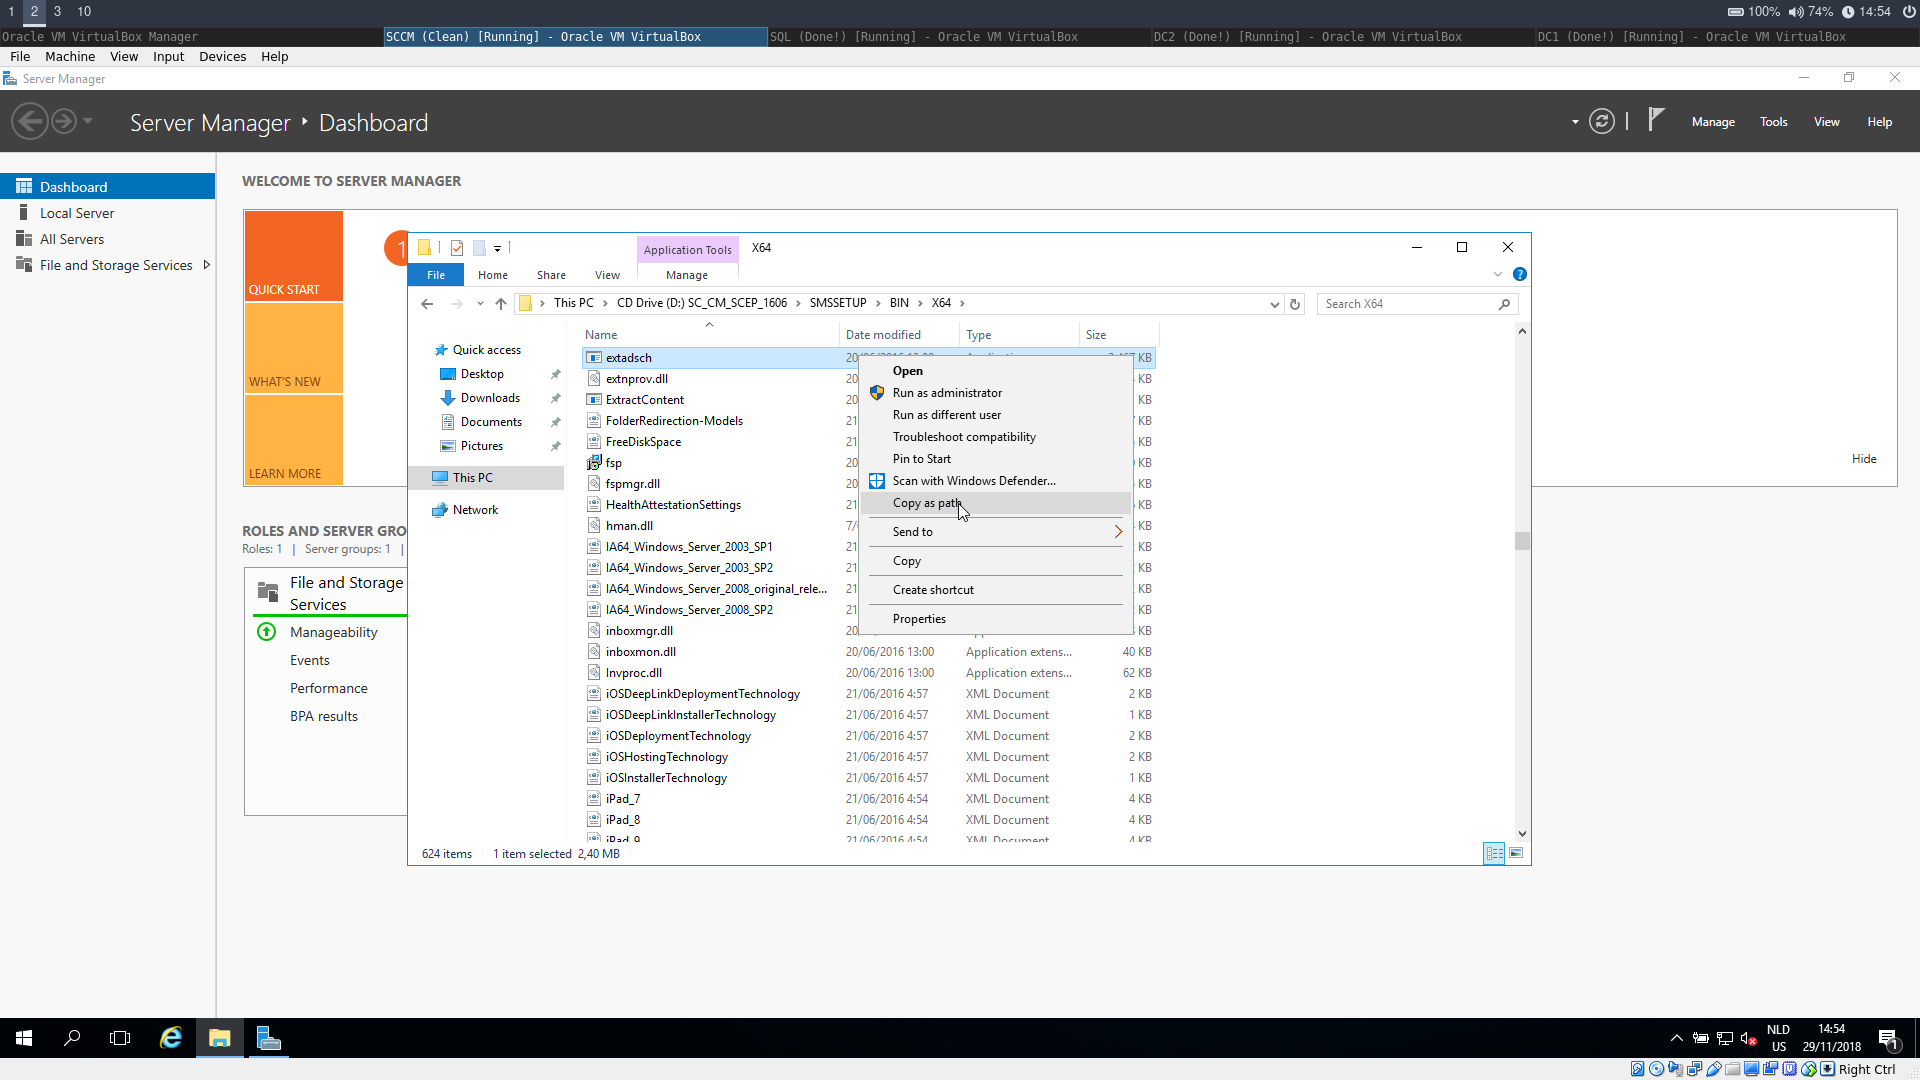
\includegraphics[width=15cm]{Pictures/SCCM/2/1543499664.png}
	
	Doe shift + rechtermuisknop op "extadsch.exe" en selecteer "Copy as path".
\end{center}

\begin{center}
	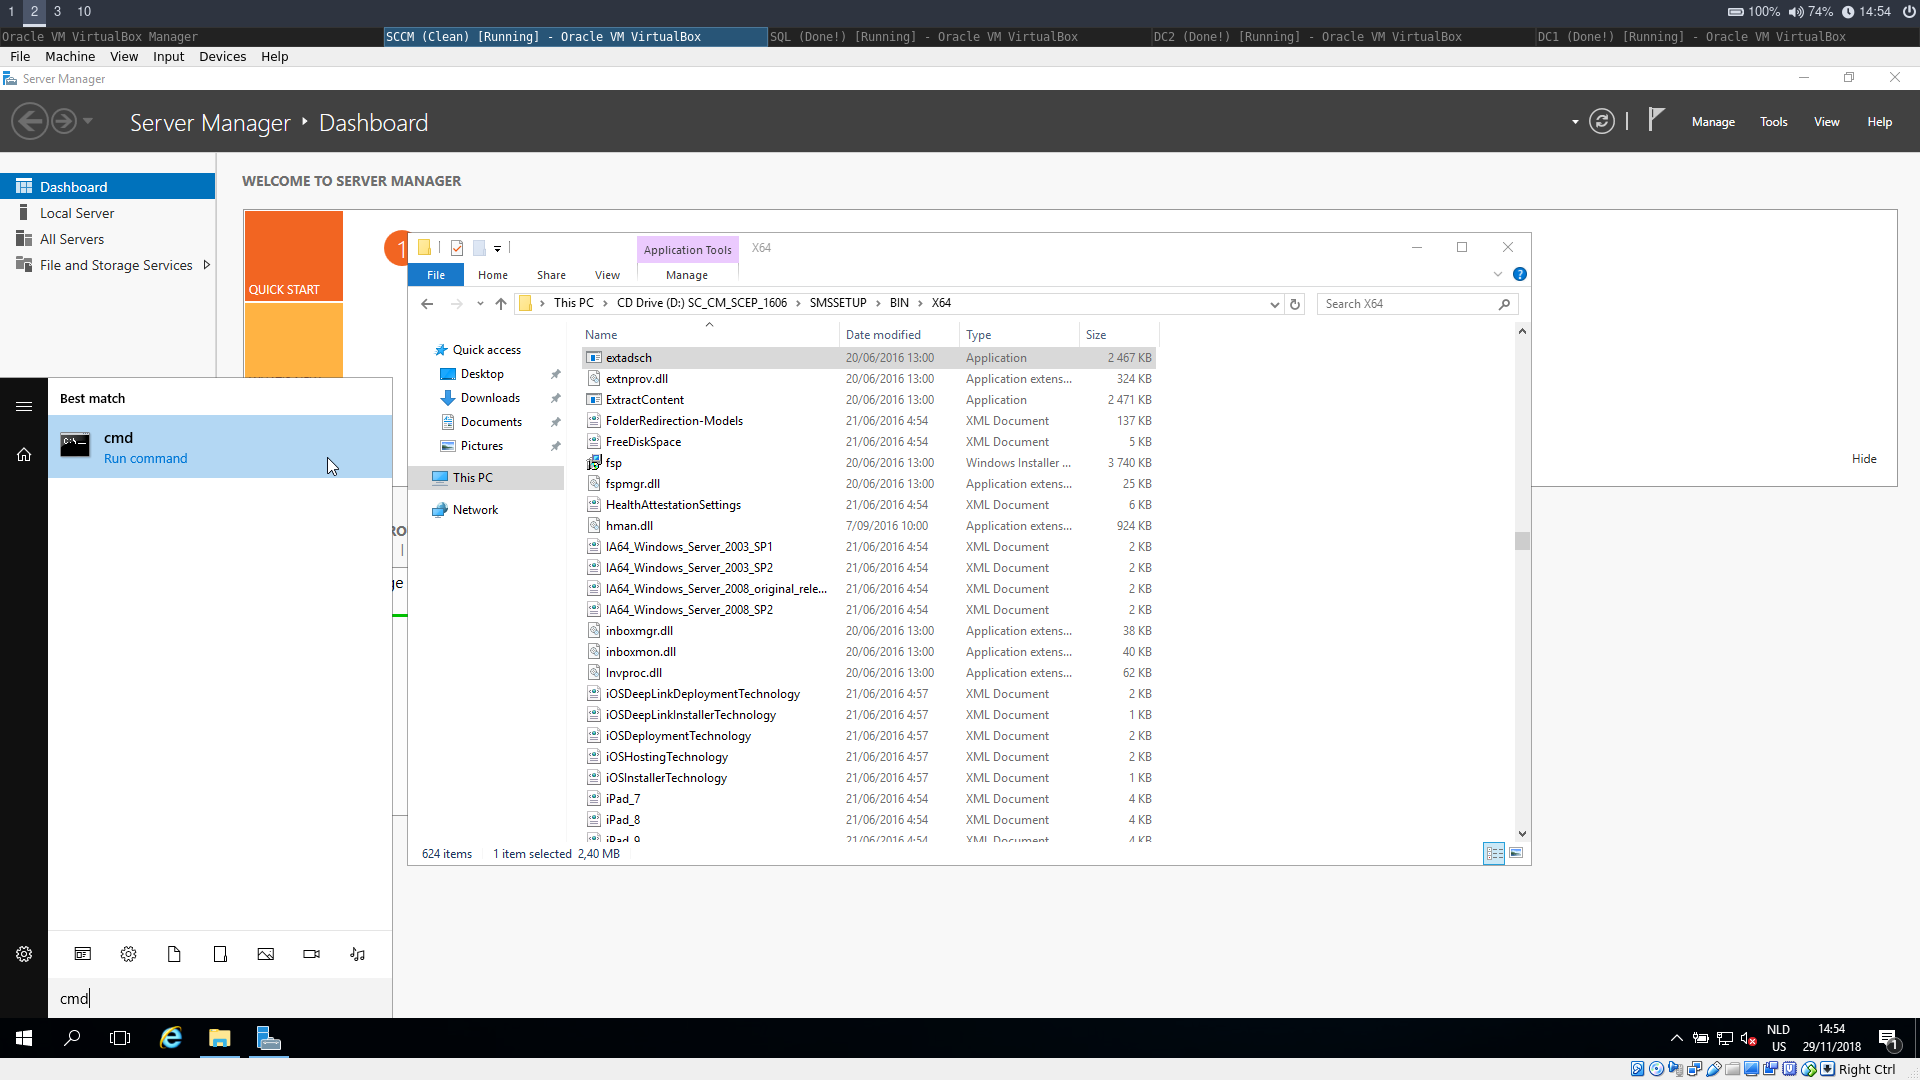
\includegraphics[width=15cm]{Pictures/SCCM/2/1543499669.png}
	
	Open een terminalvenster.
\end{center}

\begin{center}
	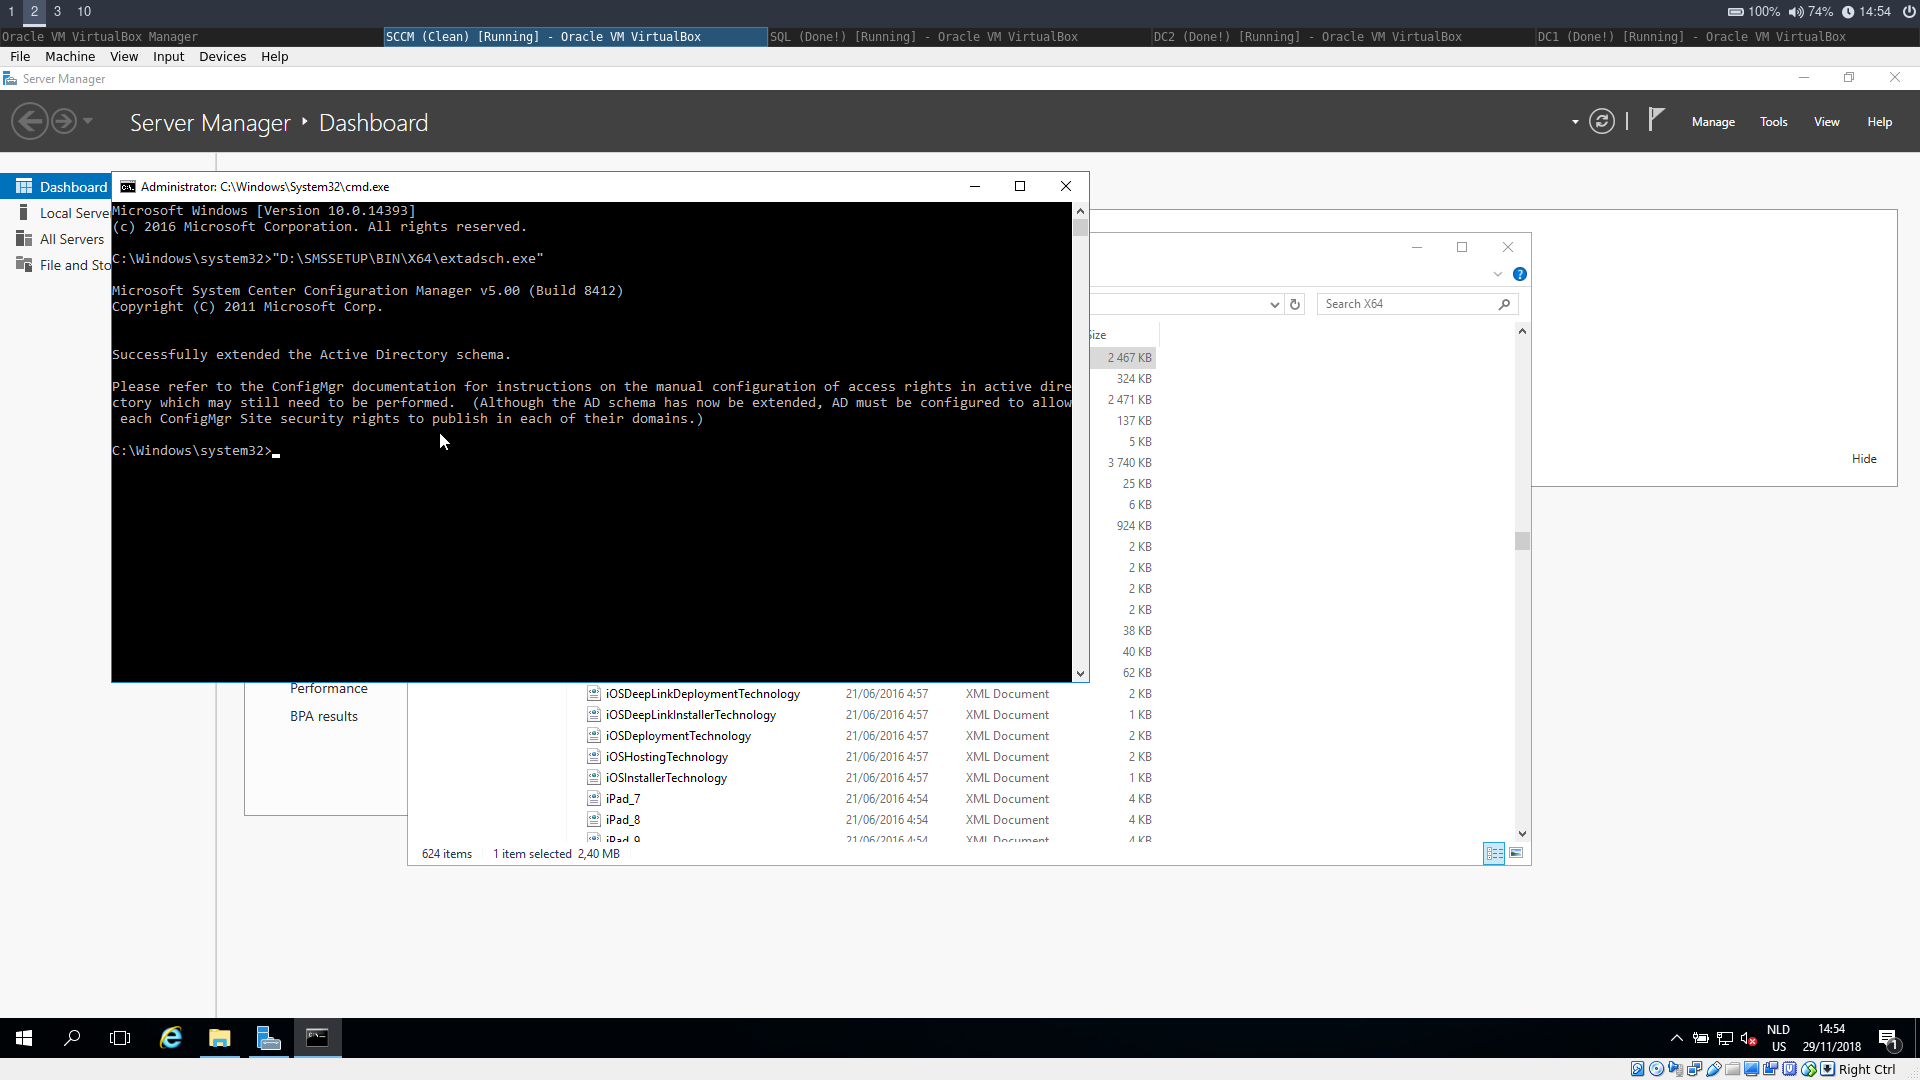
\includegraphics[width=15cm]{Pictures/SCCM/2/1543499693.png}
	
	Plak het commando van het klembord.
\end{center}

\begin{center}
	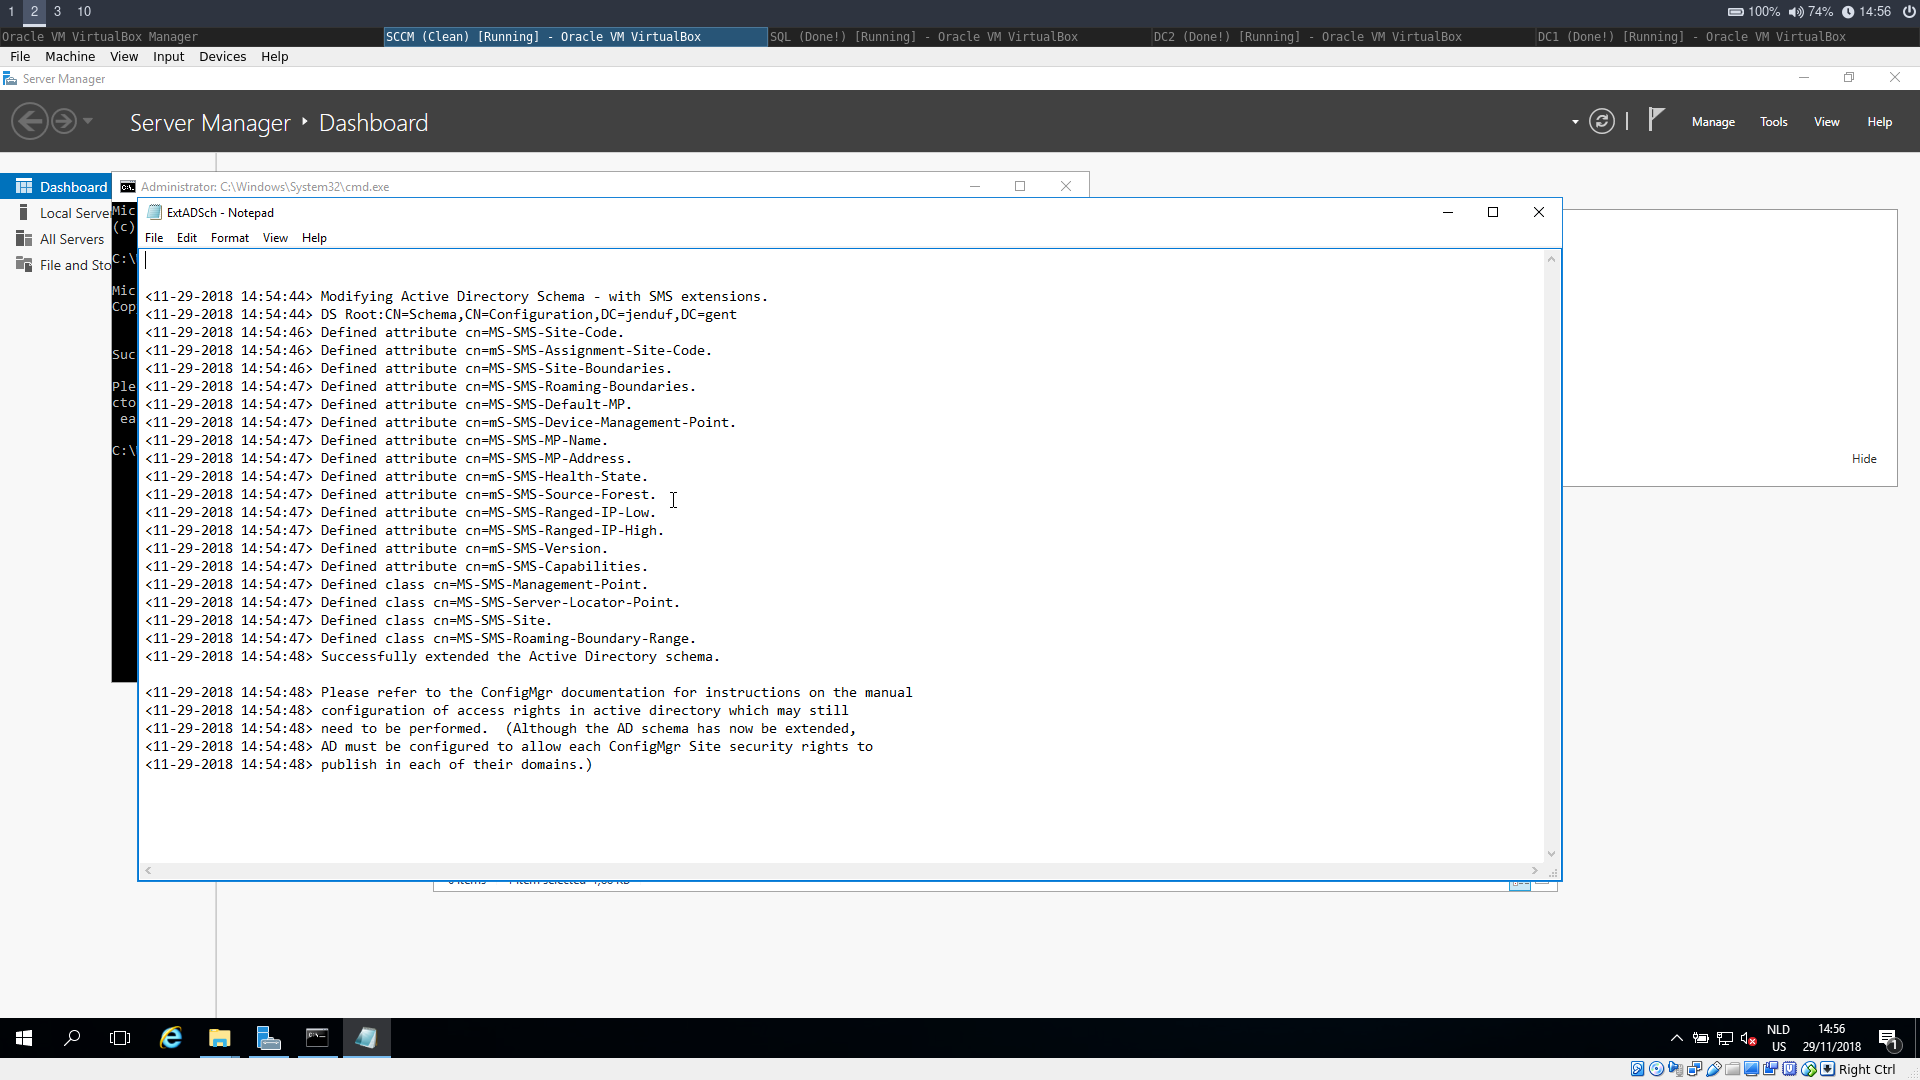
\includegraphics[width=15cm]{Pictures/SCCM/2/1543499769.png}
	
	Men kan de uitvoer controleren in "C:\textbackslash ExtADSch.log"
\end{center}
\subsection{Installatie van prerequisites}
\begin{center}
	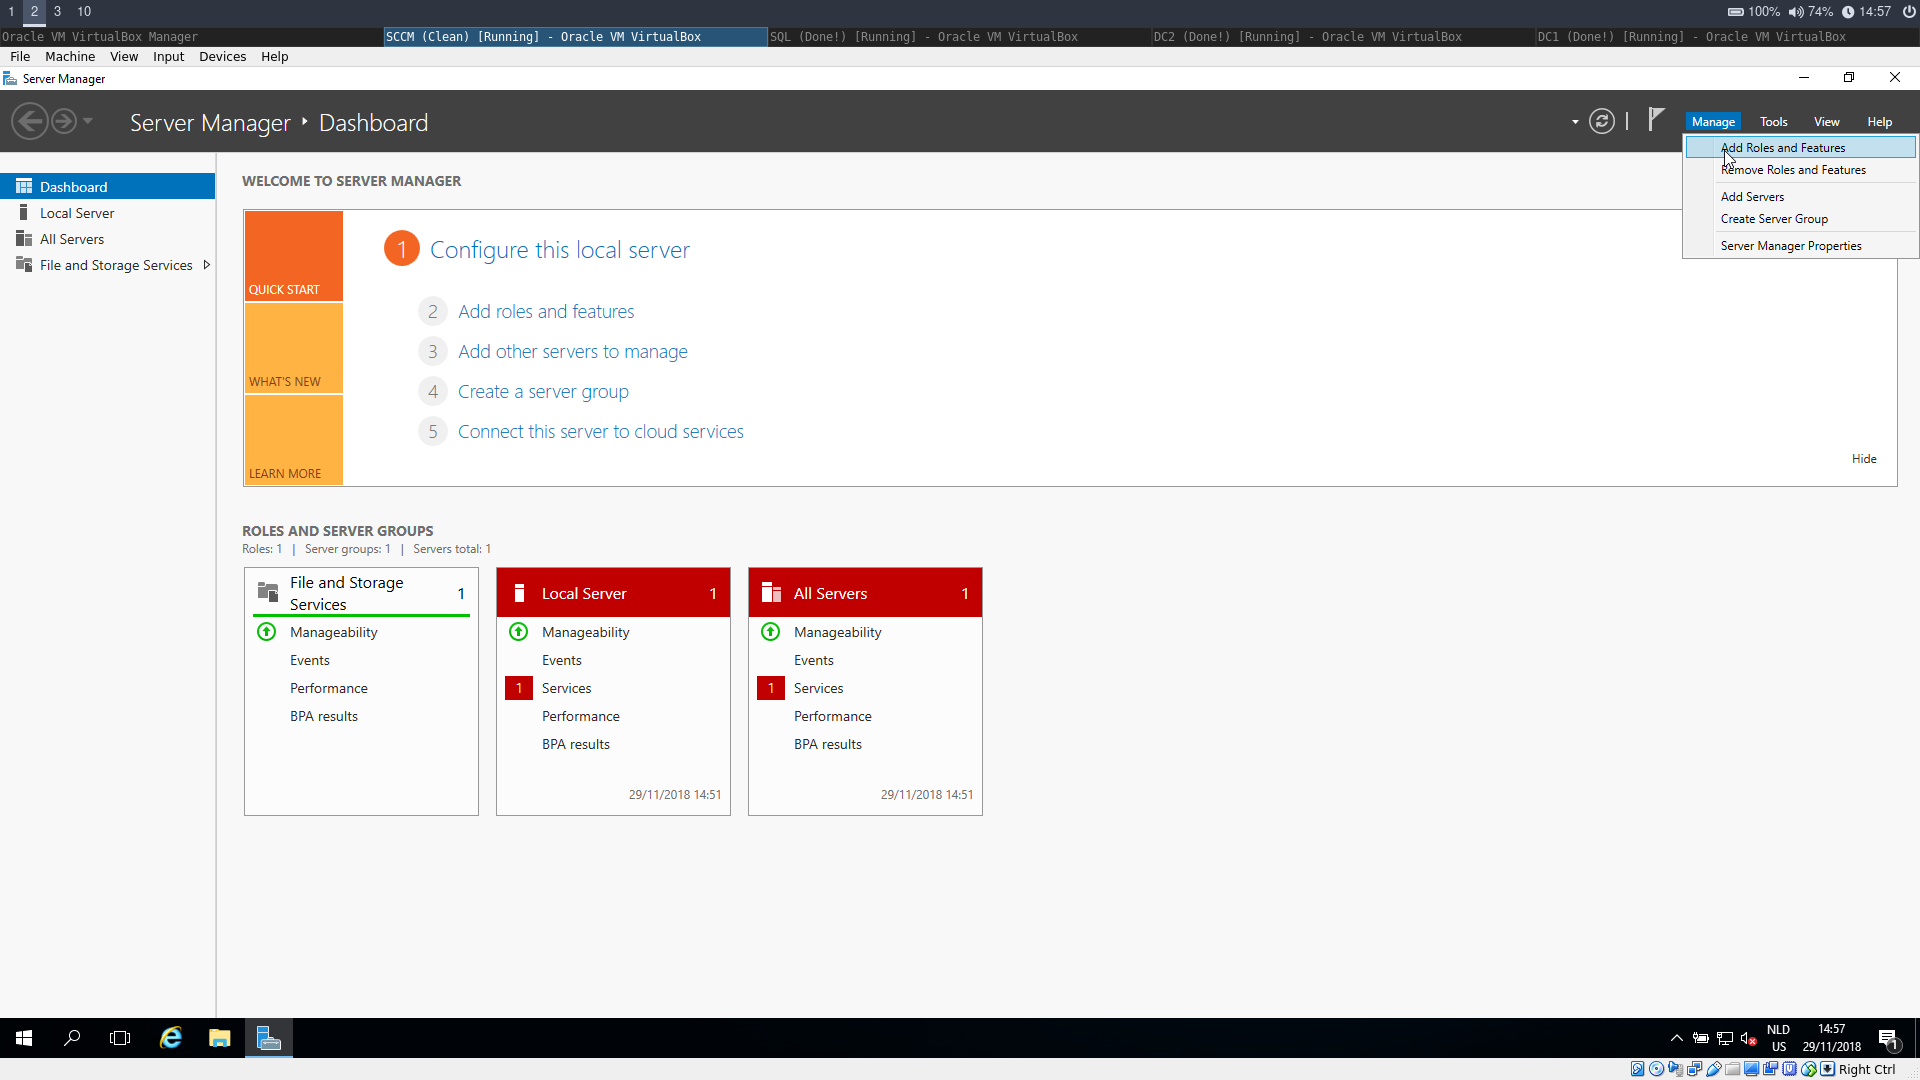
\includegraphics[width=15cm]{Pictures/SCCM/3/1543499830.png}
	
	Klik op "Add Roles and Features".
\end{center}
\begin{center}
	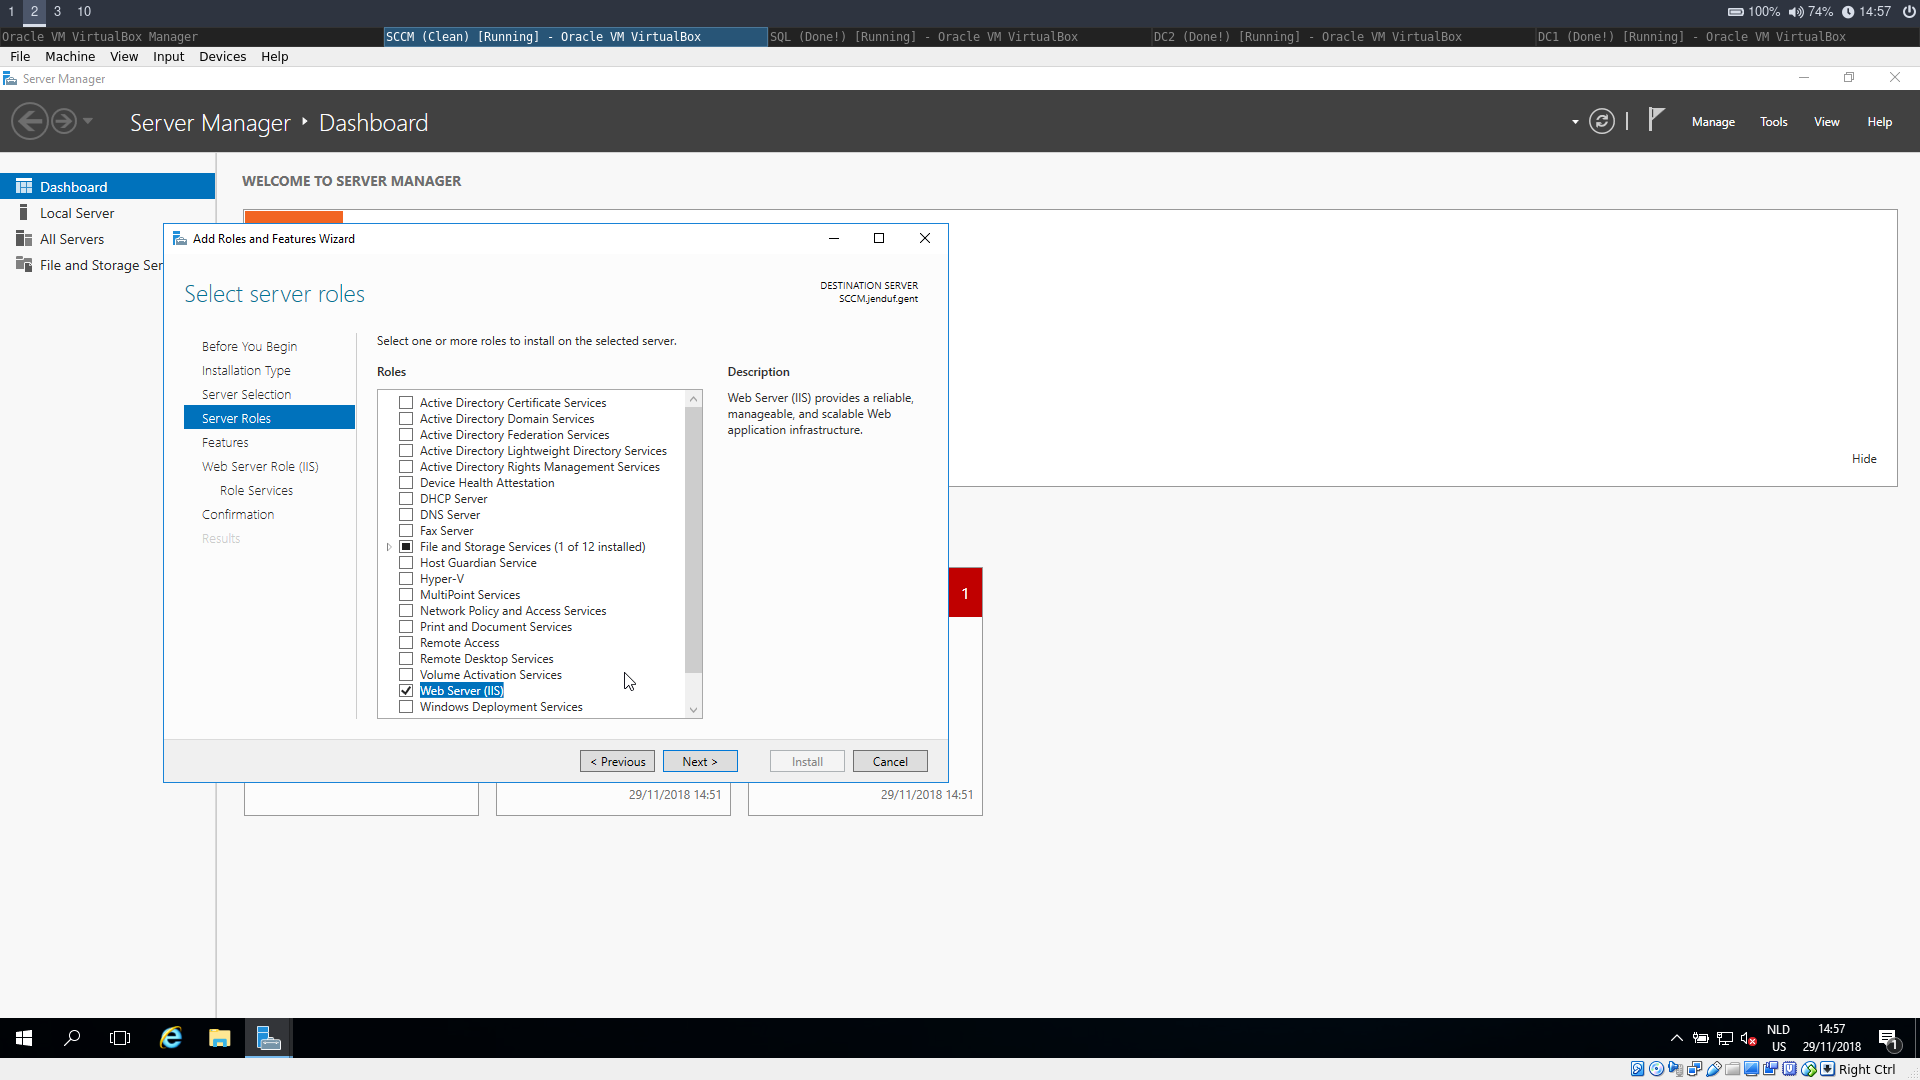
\includegraphics[width=15cm]{Pictures/SCCM/3/1543499848.png}
	
	Selecteer de "Web Server (IIS)"
\end{center}
\begin{center}
	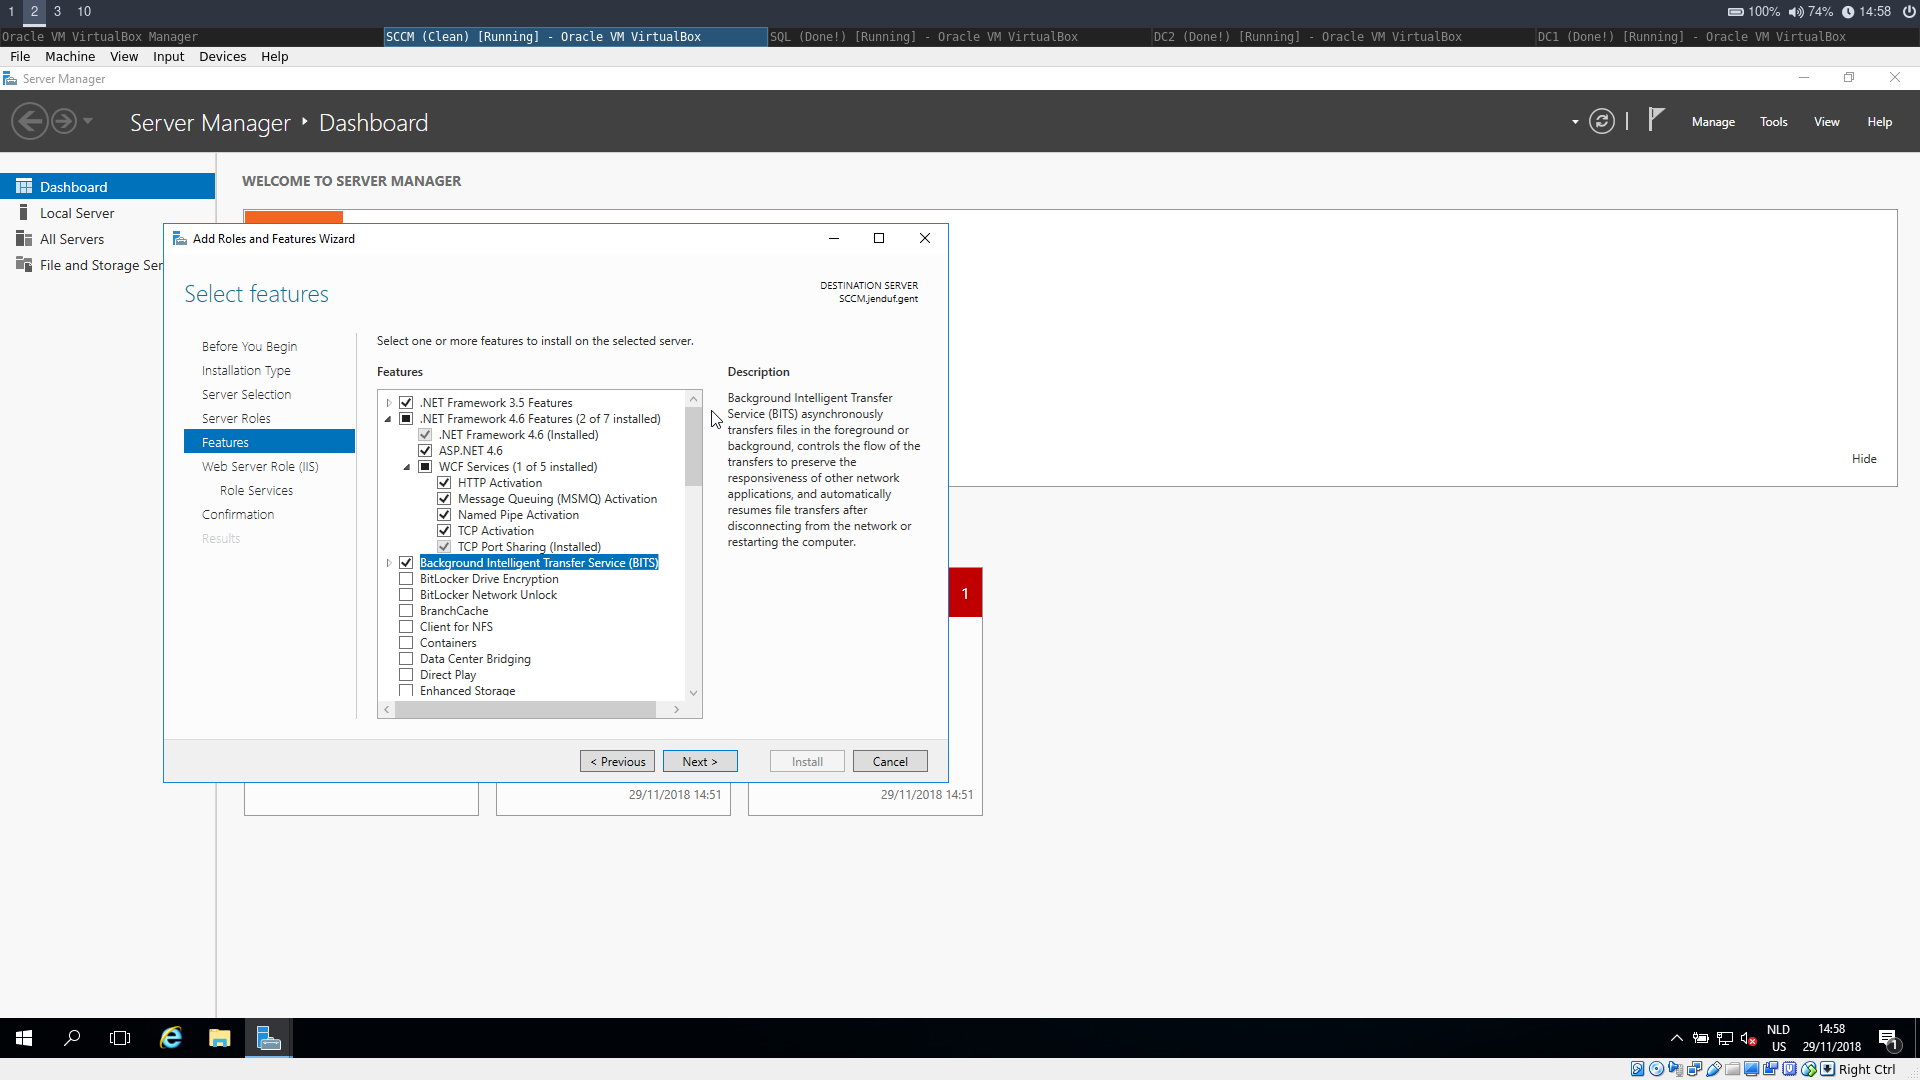
\includegraphics[width=15cm]{Pictures/SCCM/3/1543499895.png}
	
	Selecteer de aangevinkte "Features".
\end{center}
\begin{center}
	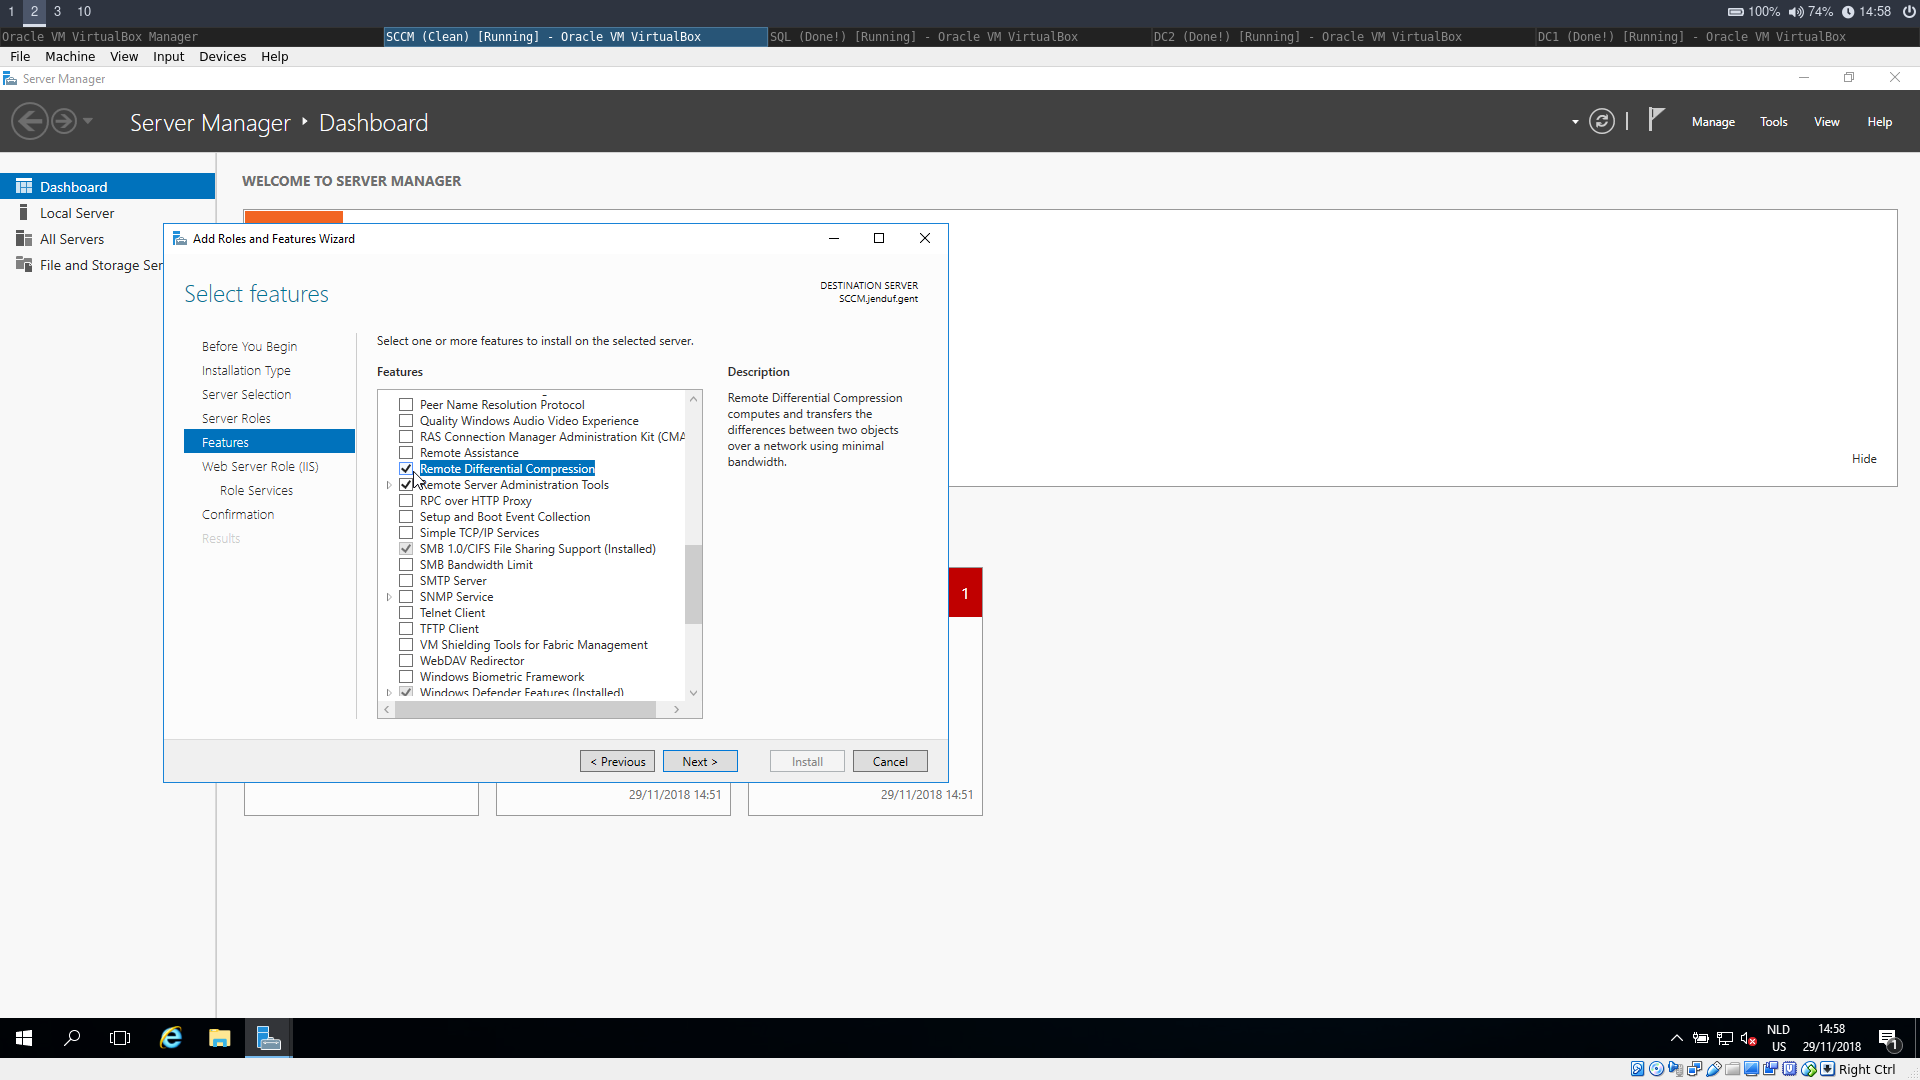
\includegraphics[width=15cm]{Pictures/SCCM/3/1543499901.png}
	
		Selecteer de aangevinkte "Features".
\end{center}
\begin{center}
	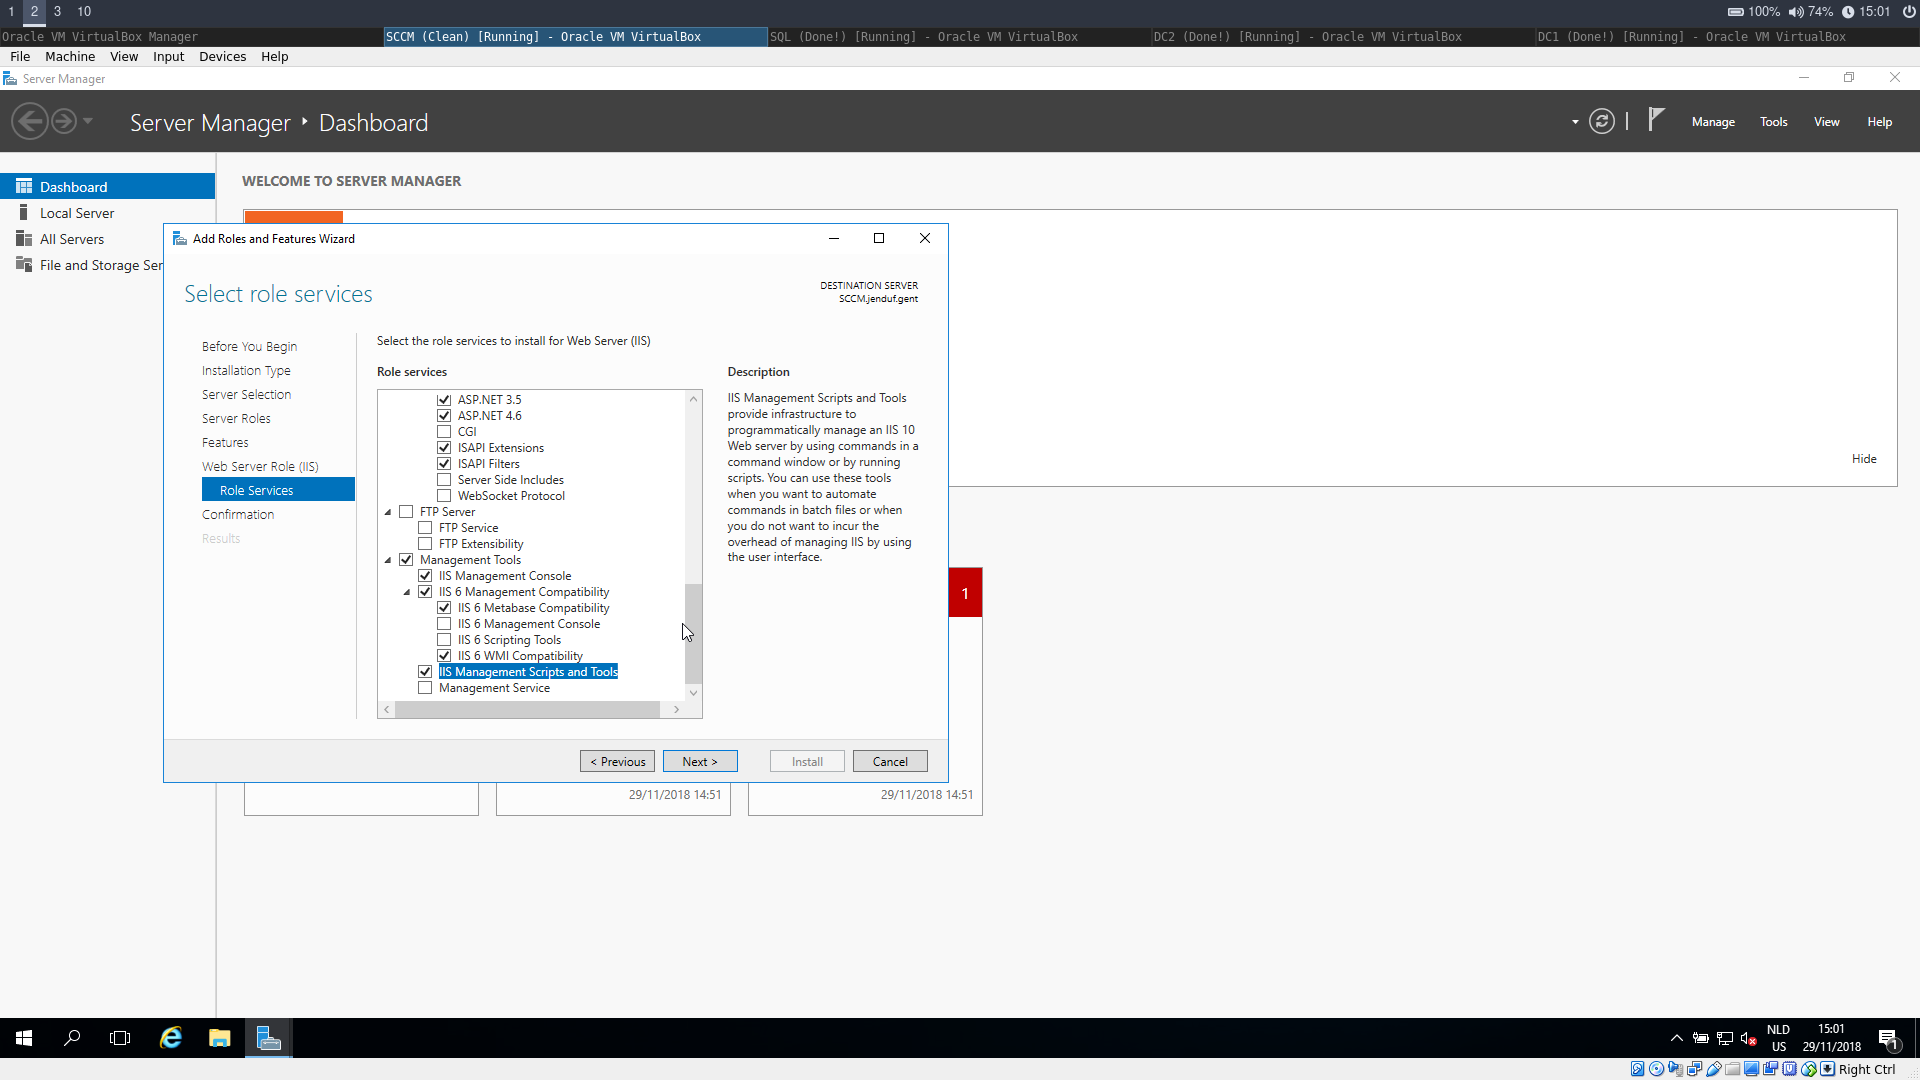
\includegraphics[width=15cm]{Pictures/SCCM/3/1543500064.png}
	
	Selecteer de volgende "Role Services".
\end{center}
\begin{center}
	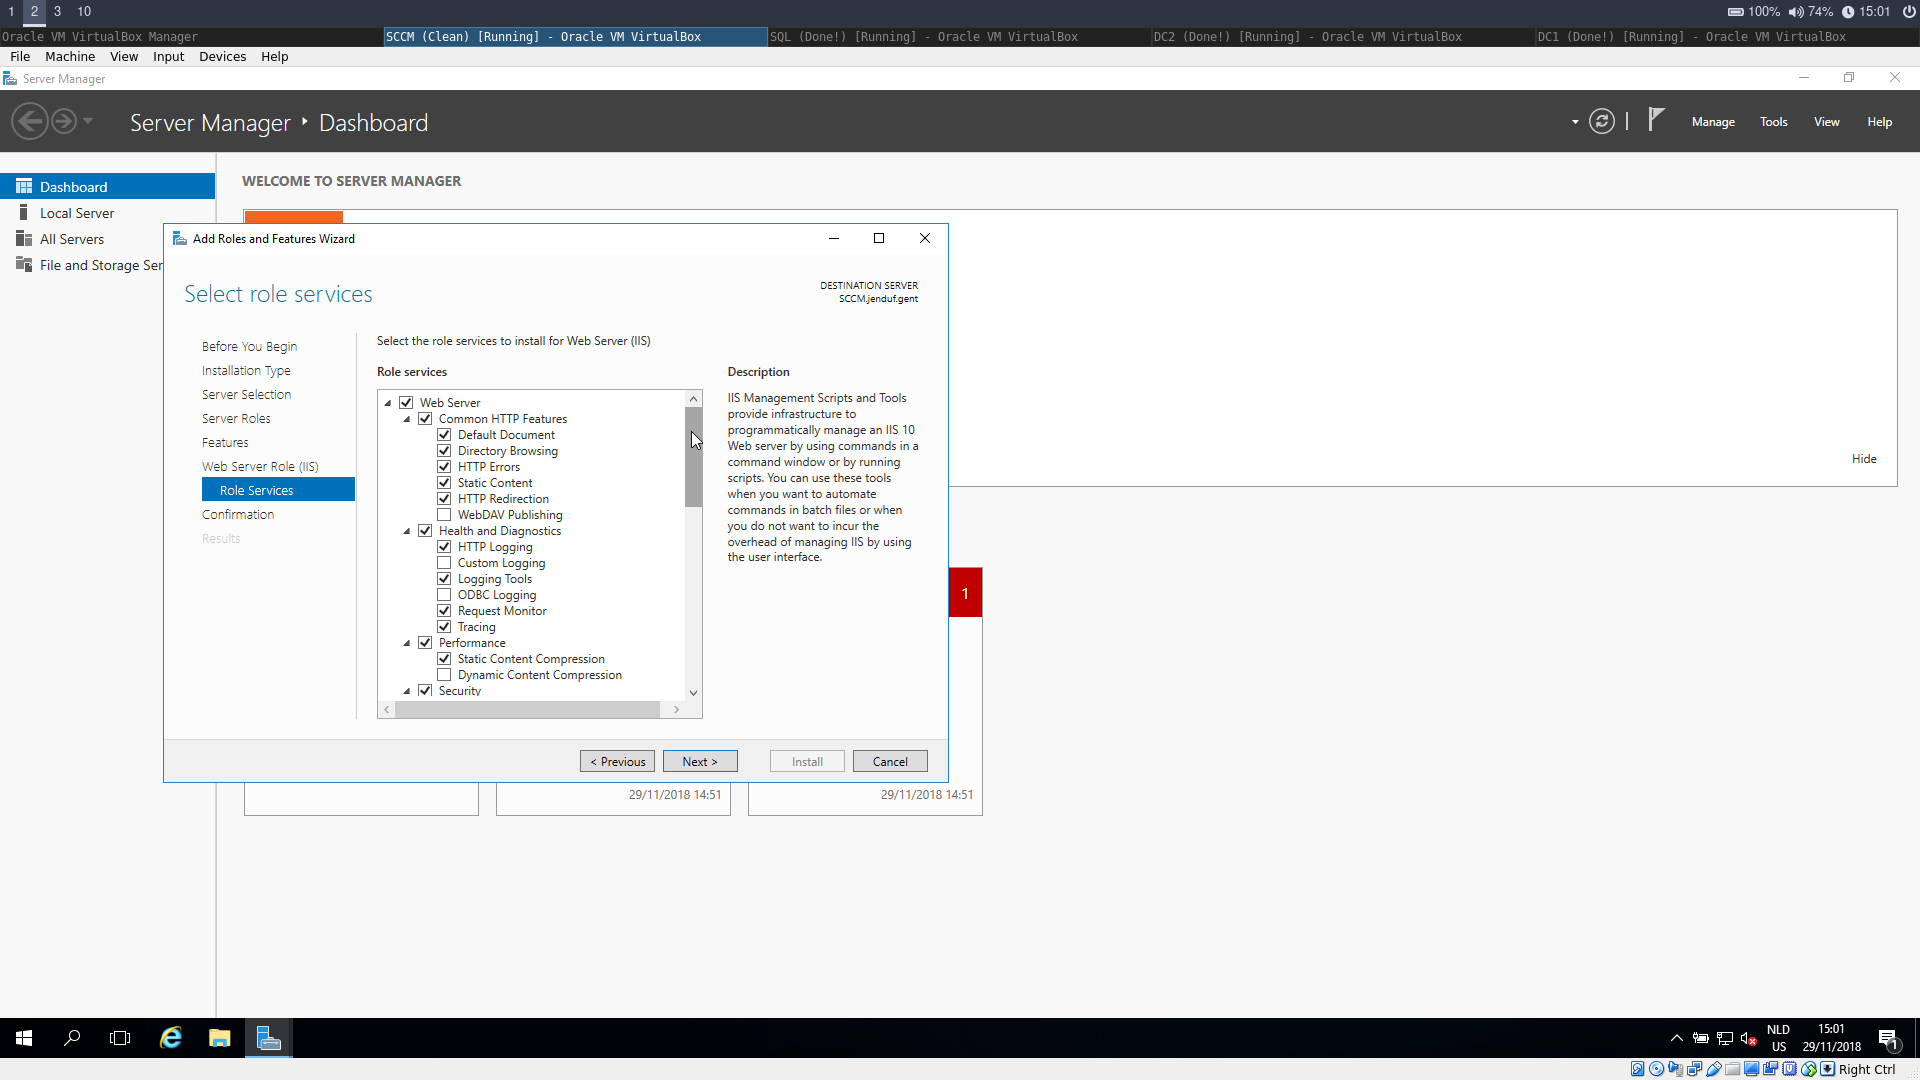
\includegraphics[width=15cm]{Pictures/SCCM/3/1543500068.png}
	
		Selecteer de volgende "Role Services".
\end{center}
\begin{center}
	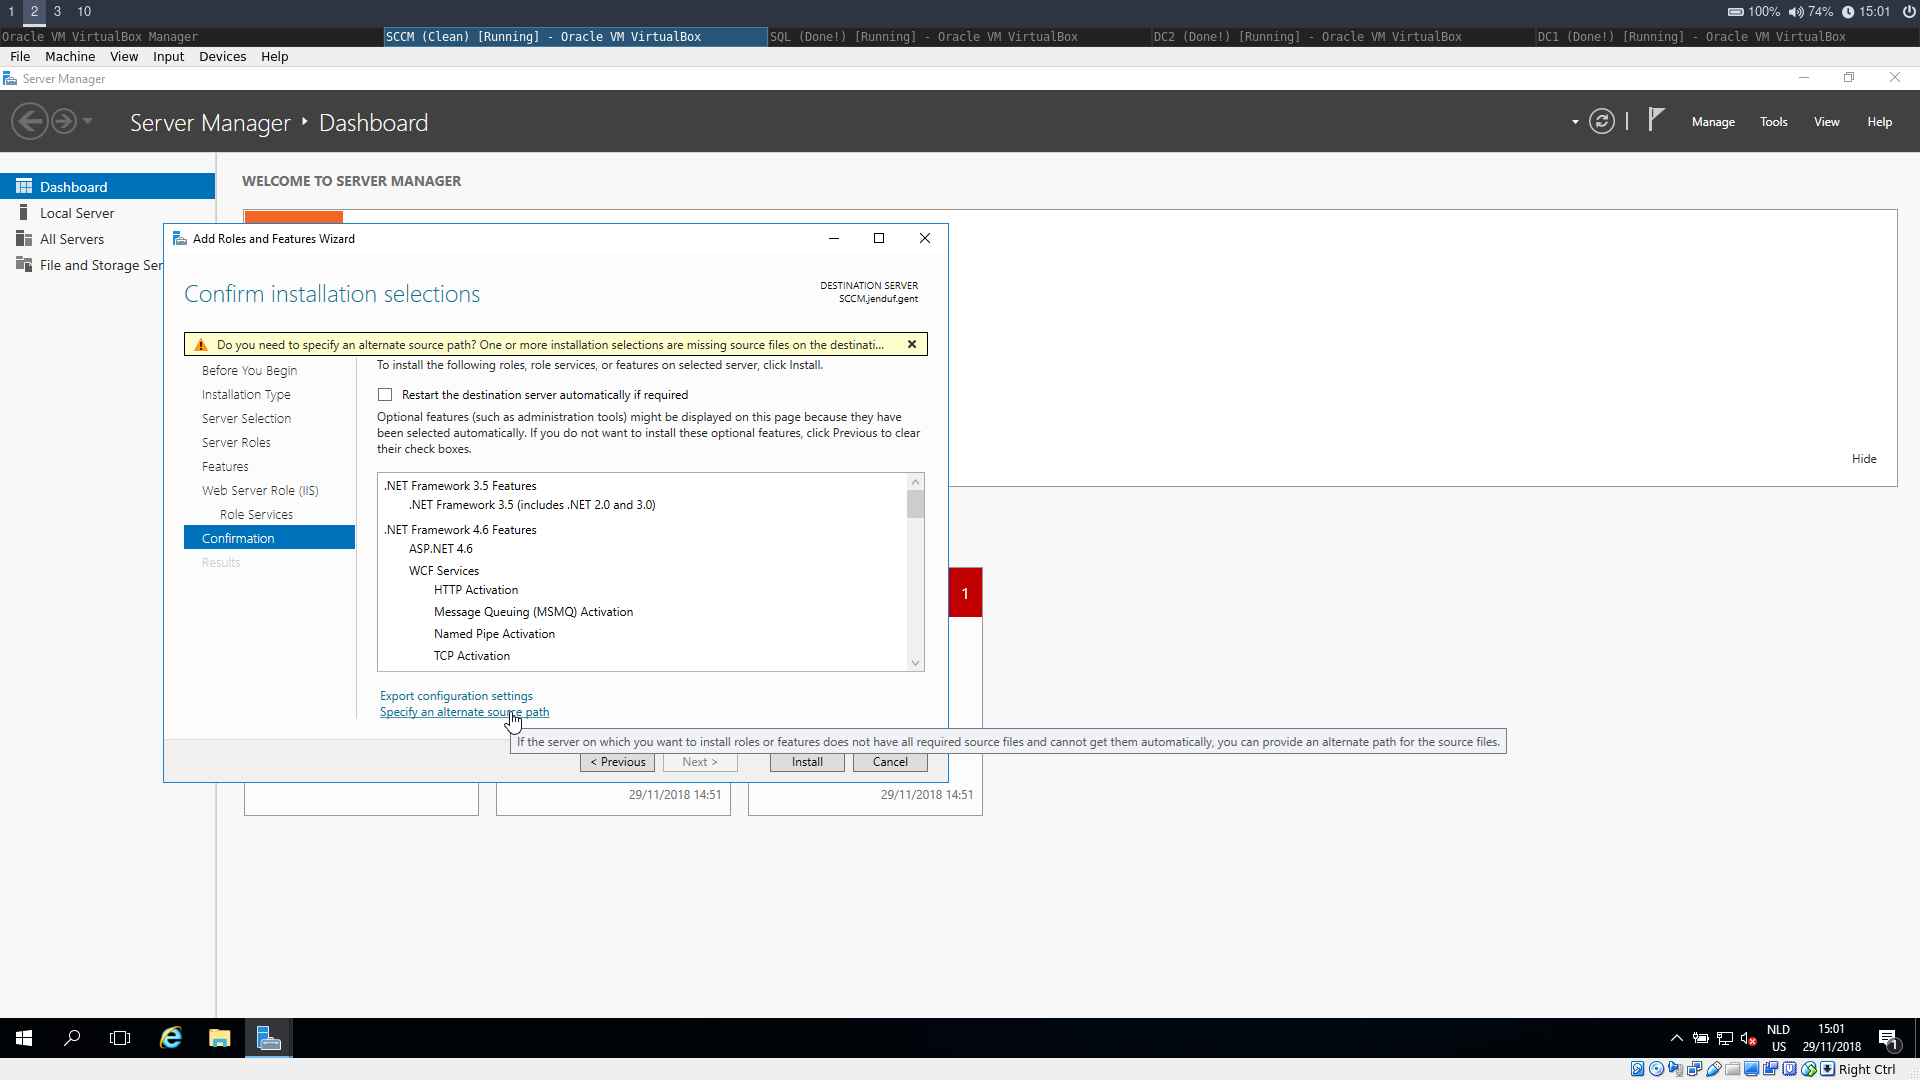
\includegraphics[width=15cm]{Pictures/SCCM/3/1543500082.png}
	
	Klik op "Specify an alternate source path".
\end{center}
\begin{center}
	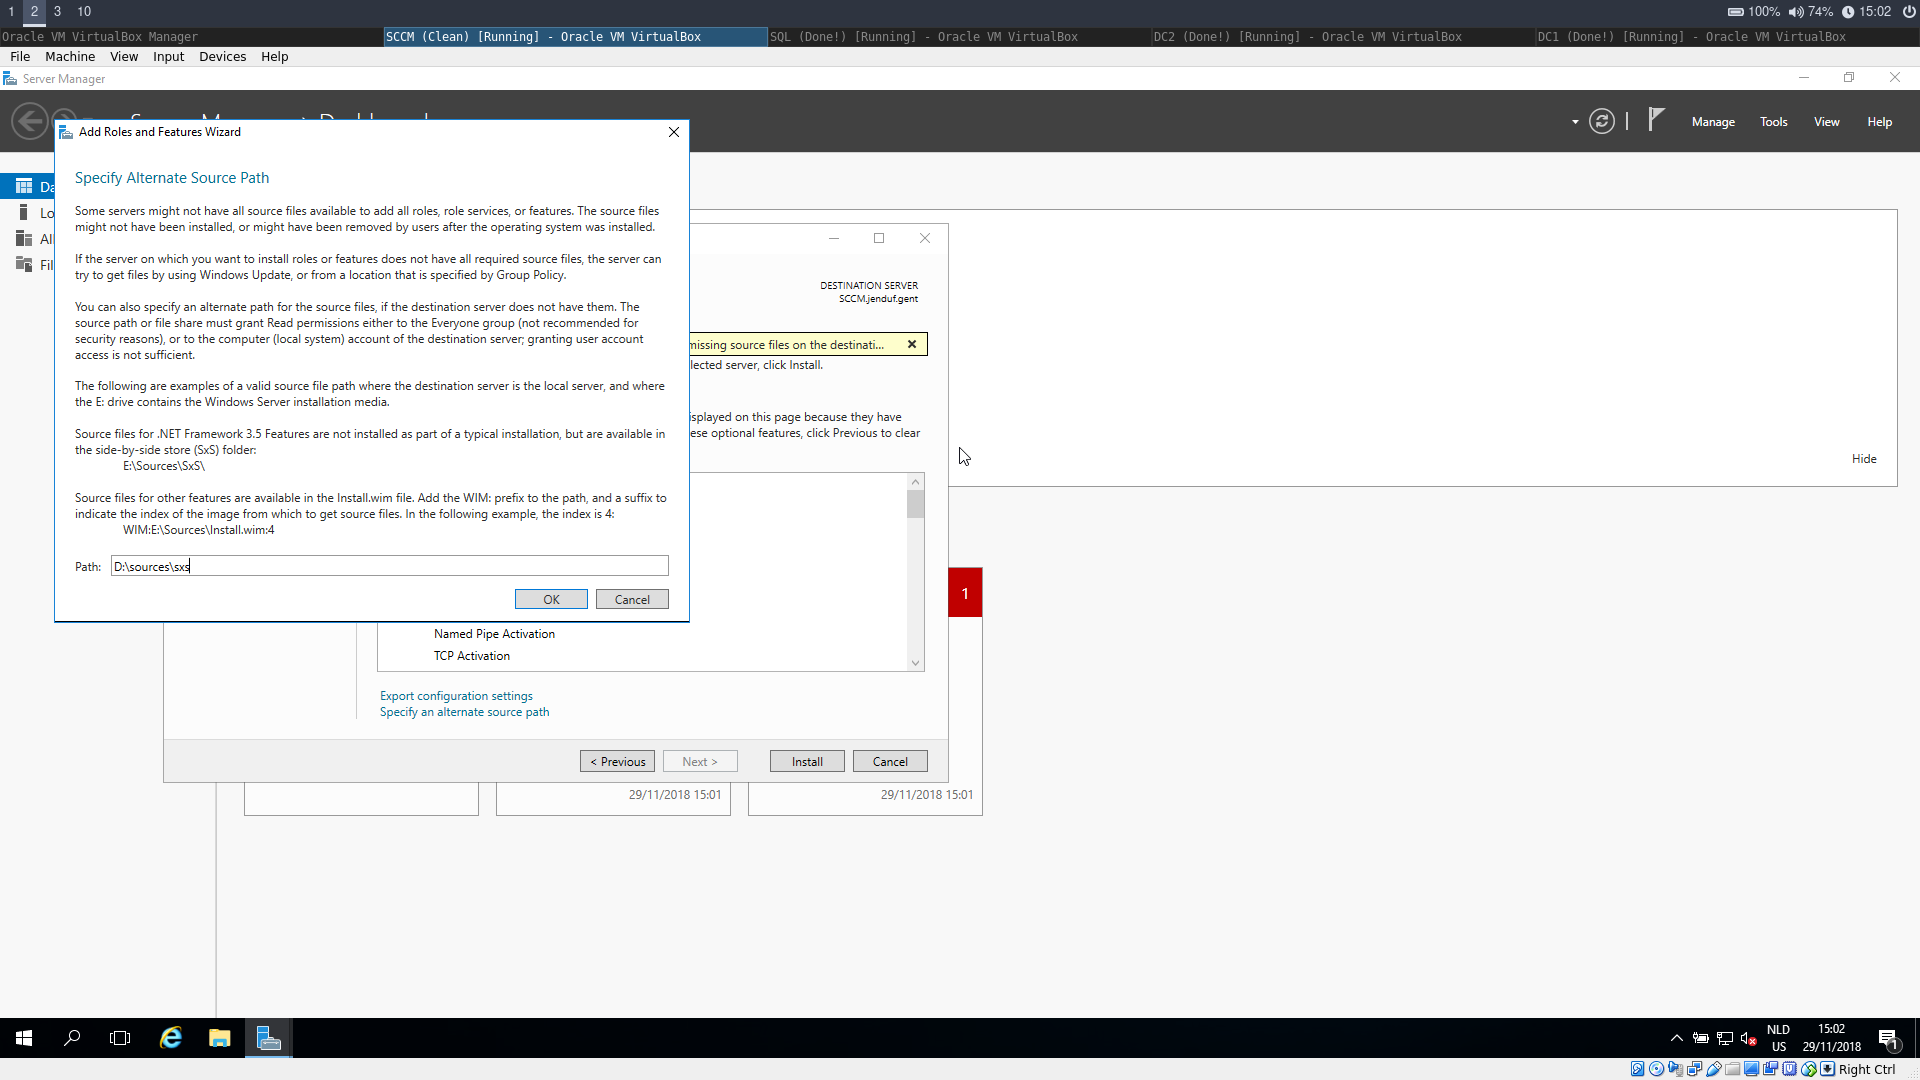
\includegraphics[width=15cm]{Pictures/SCCM/3/1543500136.png}
	
	Geef in dit veld de locatie van "sources\textbackslash SxS" in.
\end{center}
\begin{center}
	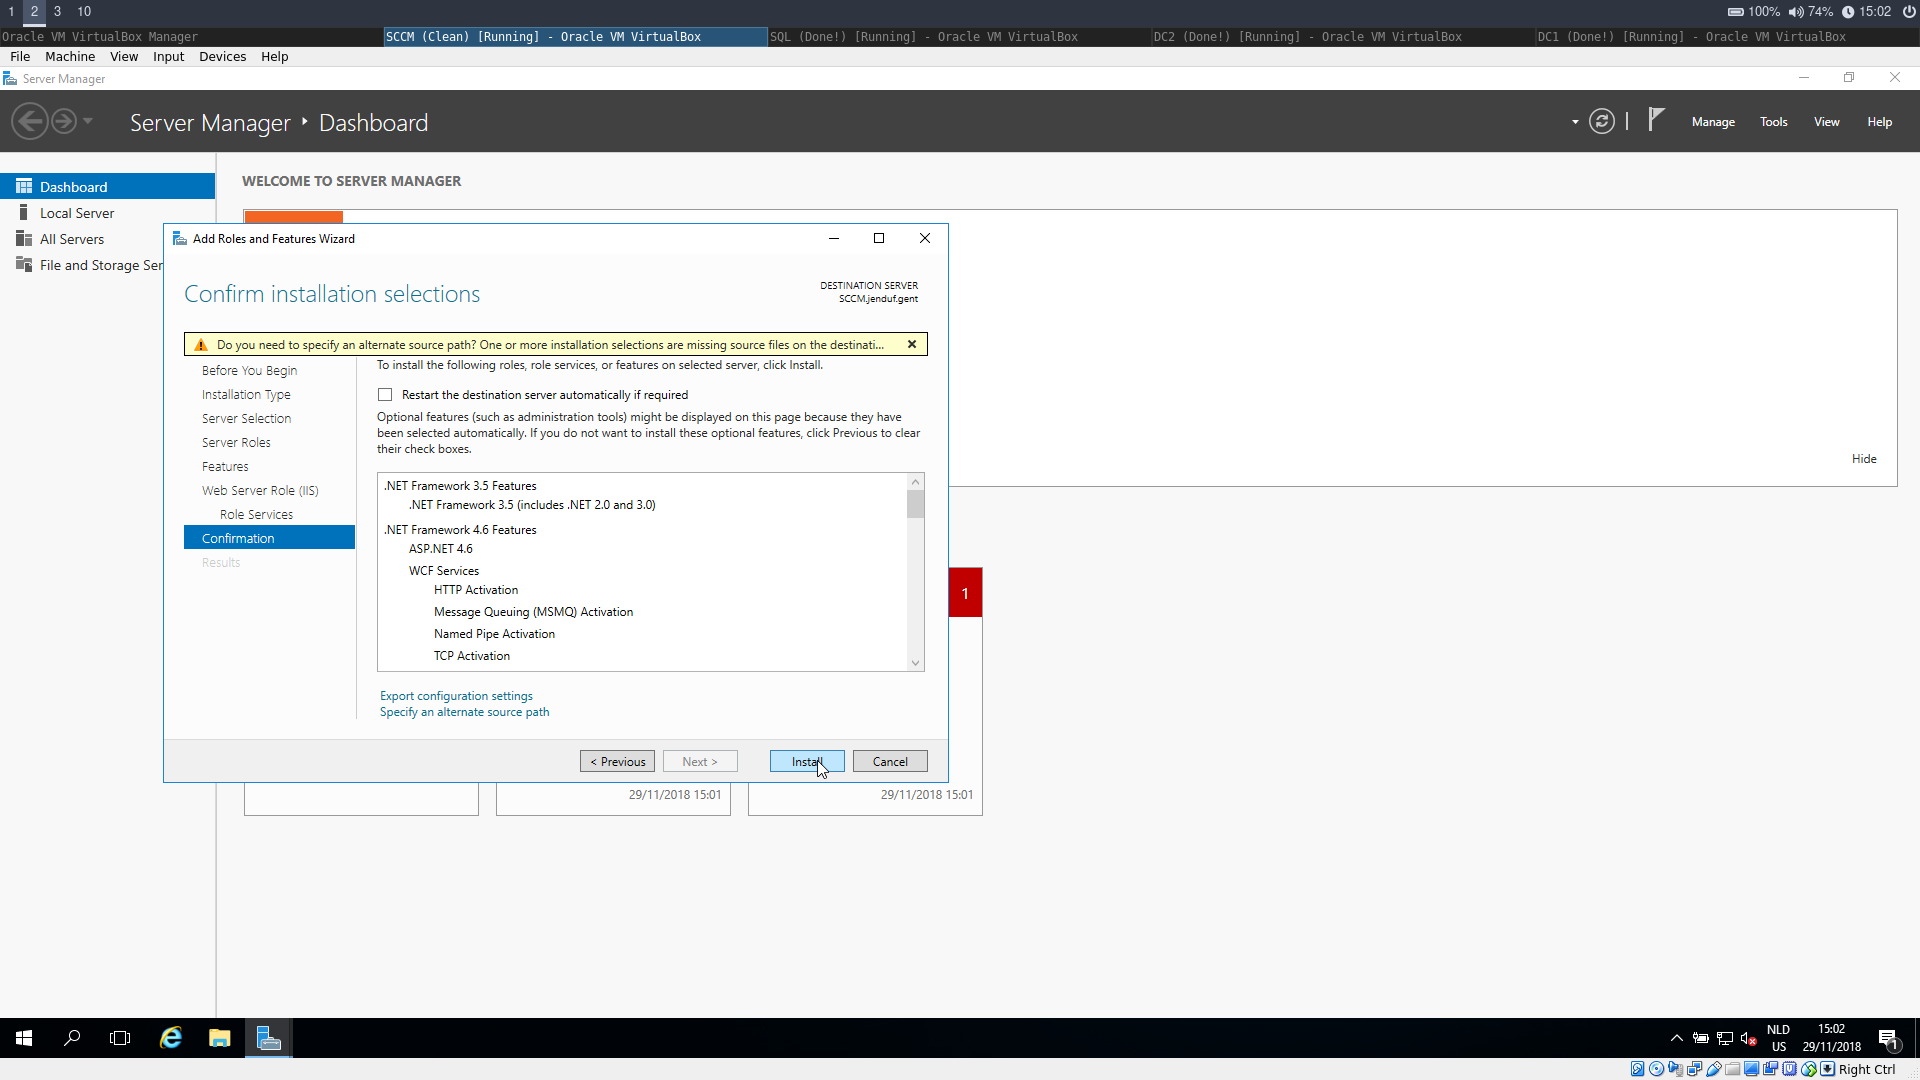
\includegraphics[width=15cm]{Pictures/SCCM/3/1543500140.png}
	
	Start de installatie.
\end{center}
\begin{center}
	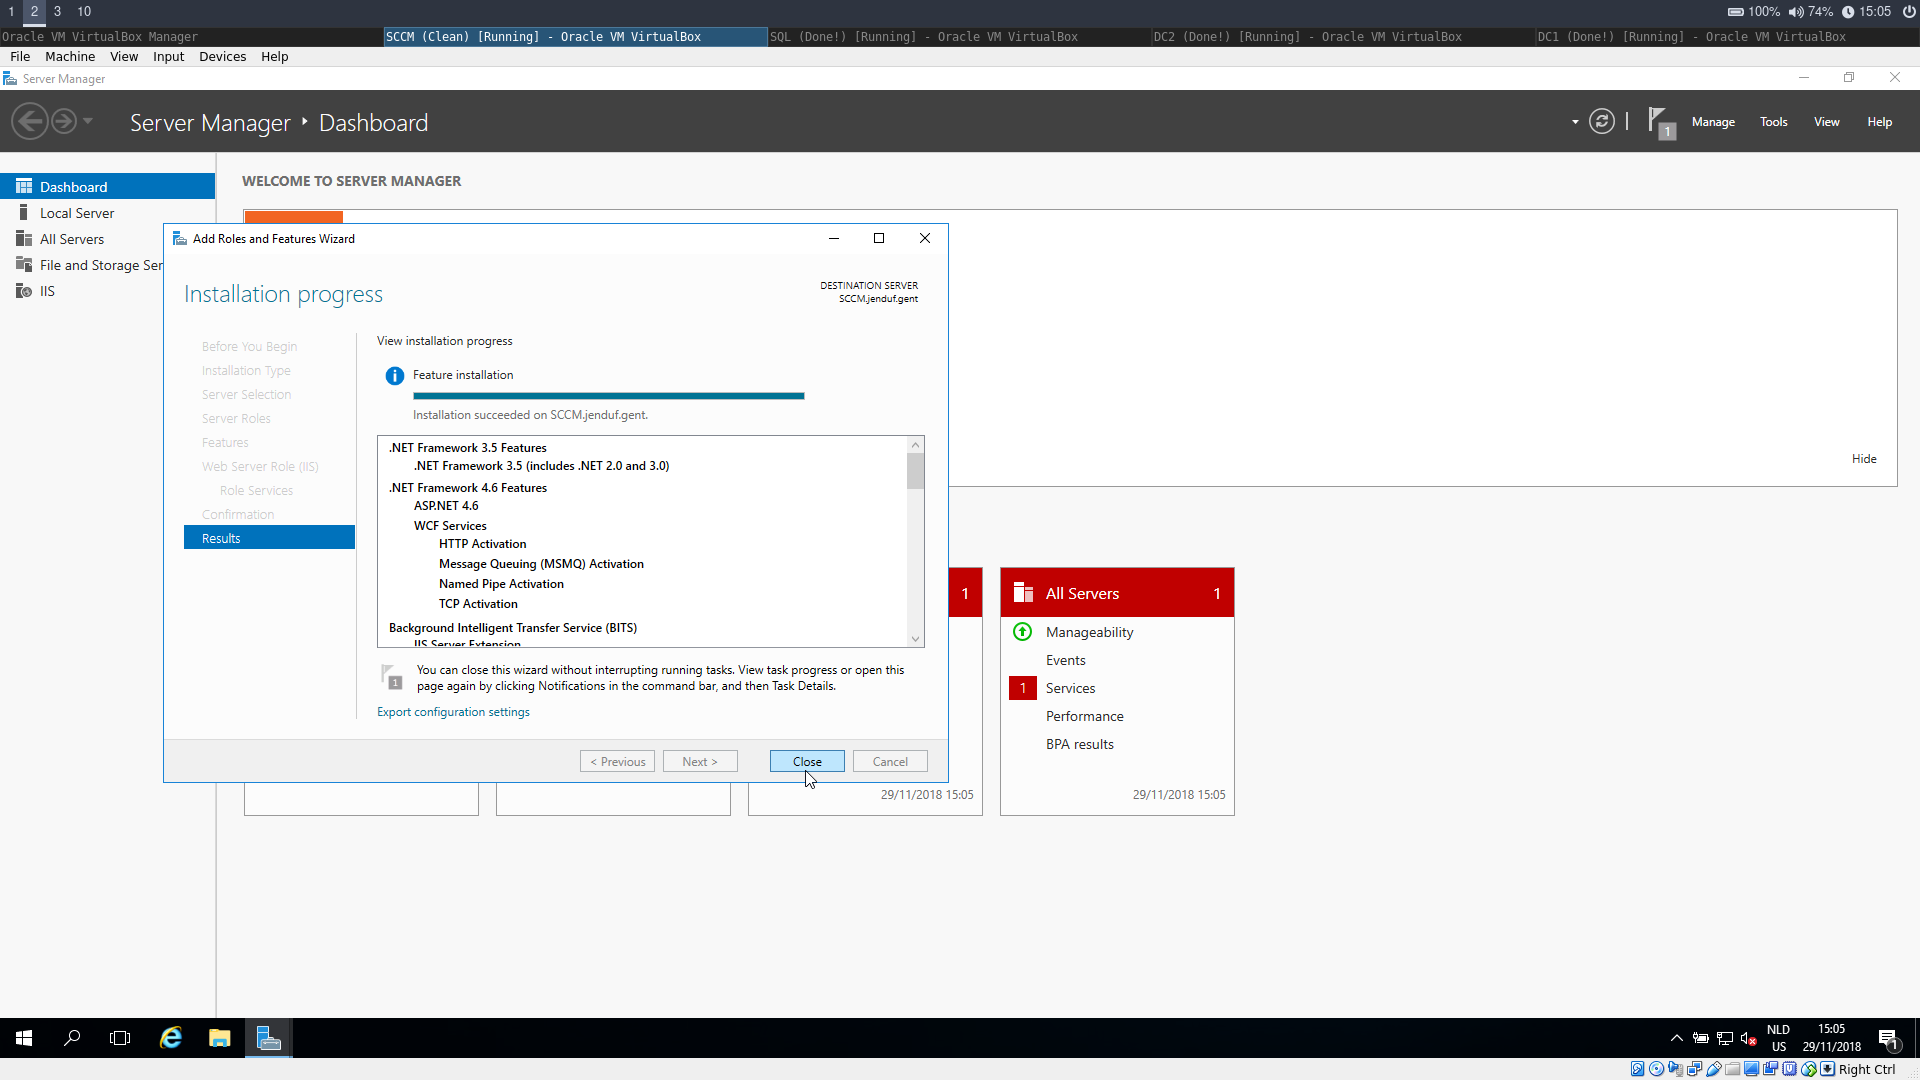
\includegraphics[width=15cm]{Pictures/SCCM/3/1543500314.png}
	
	De installatie is voltooid. U mag dit venster sluiten.
\end{center}
\subsection{Installatie van Windows Assessment and Deployment Kit}
\begin{center}
	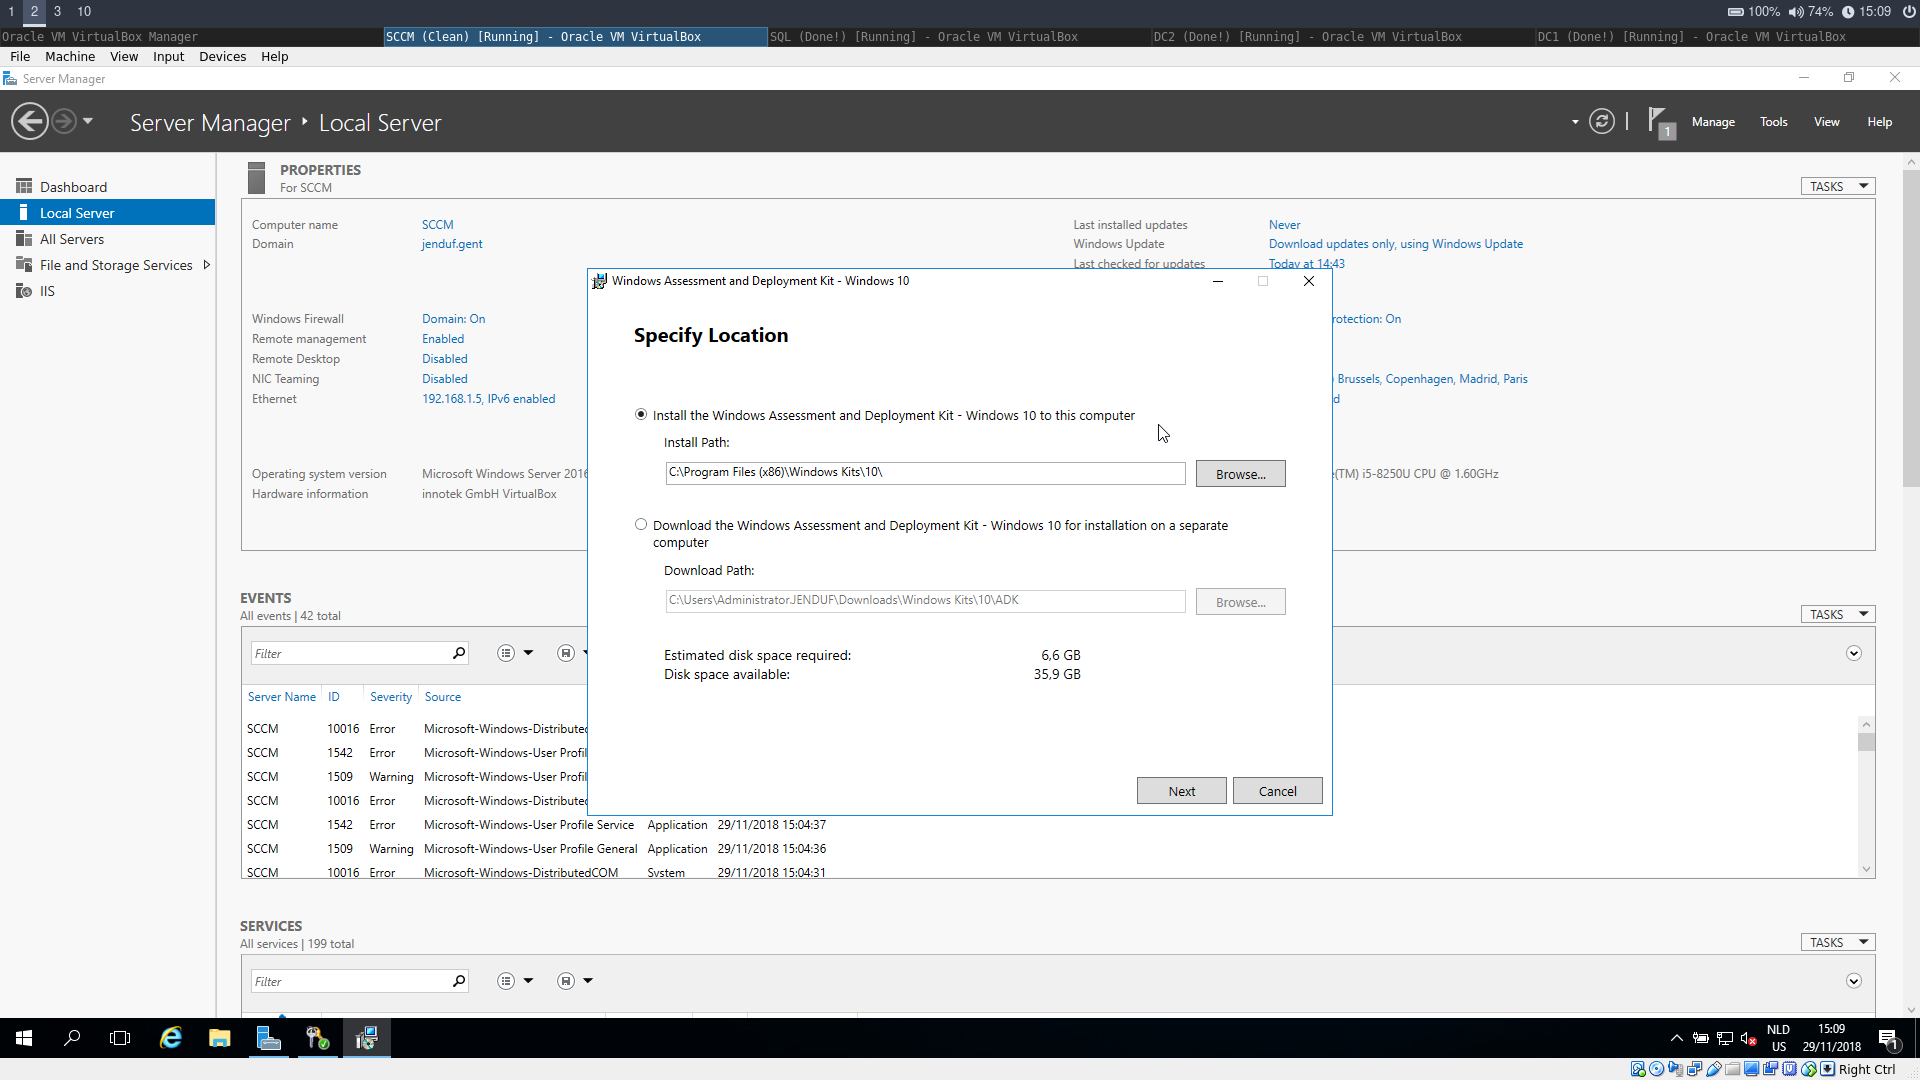
\includegraphics[width=15cm]{Pictures/SCCM/4/1543500545.png}
	
	Klik op "Next".
\end{center}
\begin{center}
	\includegraphics[width=15cm]{Pictures/SCCM/4/1543500555.png}
	
	Selecteer "No".
\end{center}
\begin{center}
	\includegraphics[width=15cm]{Pictures/SCCM/4/1543500557.png}
	
	Ga akkoord met de licentievoorwaarden.
\end{center}
\begin{center}
	\includegraphics[width=15cm]{Pictures/SCCM/4/1543500577.png}
	
	Vink de aangeduide "features" aan.
\end{center}
\begin{center}
	\includegraphics[width=15cm]{Pictures/SCCM/4/1543500666.png}
	
	De installatie is succesvol gestart.
\end{center}
\begin{center}
	\includegraphics[width=15cm]{Pictures/SCCM/4/1543501810.png}
	
	De installatie is succesvol voltooid. U mag dit venster sluiten.
\end{center}
\subsection{Installatie WSUS}
\begin{center}
	\includegraphics[width=15cm]{Pictures/SCCM/5/1543504348.png}
	
	Voeg de "Server Role" "Windows Server Update Service" toe.
\end{center}
\begin{center}
	\includegraphics[width=15cm]{Pictures/SCCM/5/1543504358.png}
	
	Vink de aangeduide "Role Services" aan. 
\end{center}
\begin{center}
	\includegraphics[width=15cm]{Pictures/SCCM/5/1543504368.png}
	
	Verwijs naar een bestaande map voor het bewaren van de updates.
\end{center}
\begin{center}
	\includegraphics[width=15cm]{Pictures/SCCM/5/1543504391.png}
	
	Verbind met de SQL Server op de server "SCCM.jenduf.gent".
\end{center}
\begin{center}
	\includegraphics[width=15cm]{Pictures/SCCM/5/1543504396.png}
	
	Start de installatie.
\end{center}
\subsection{Installatie SCCM}
\begin{center}
\includegraphics[width=15cm]{Pictures/SCCM/6/1543502369.png}

Klik op "Install".
\end{center}
\begin{center}
\includegraphics[width=15cm]{Pictures/SCCM/6/1543502380.png}

Klik op "Next".
\end{center}
\begin{center}
\includegraphics[width=15cm]{Pictures/SCCM/6/1543502389.png}

Klik op "Next".
\end{center}
\begin{center}
\includegraphics[width=15cm]{Pictures/SCCM/6/1543502394.png}

Installeer SCCM als een evaluatieversie.
\end{center}
\begin{center}
\includegraphics[width=15cm]{Pictures/SCCM/6/1543502403.png}

Ga akkoord met de licentievoorwaarden.
\end{center}
\begin{center}
\includegraphics[width=15cm]{Pictures/SCCM/6/1543502522.png}

Download de benodigde bestanden en klik op "Next".
\end{center}
\begin{center}
\includegraphics[width=15cm]{Pictures/SCCM/6/1543502769.png}

Even geduld tot het downloaden van de bestanden voltooid is.
\end{center}
\begin{center}
\includegraphics[width=15cm]{Pictures/SCCM/6/1543502844.png}

Selecteer de Engelse taal.
\end{center}
\begin{center}
\includegraphics[width=15cm]{Pictures/SCCM/6/1543502847.png}

Selecteer de Engelse taal.
\end{center}
\begin{center}
\includegraphics[width=15cm]{Pictures/SCCM/6/1543502871.png}

Geef als "Site Code" "BEL" in en als "Site Name" "jenduf.gent" en ga verder met de installatiewizard.
\end{center}
\begin{center}
\includegraphics[width=15cm]{Pictures/SCCM/6/1543502888.png}

Selecteer "Install the primary site as a stand-alone server".
\end{center}
\begin{center}
\includegraphics[width=15cm]{Pictures/SCCM/6/1543502894.png}

Klik op "Yes".
\end{center}
\begin{center}
\includegraphics[width=15cm]{Pictures/SCCM/6/1543504659.png}

Geef als "SQL Server Name" "SCCM.jenduf.gent" in en ga verder.
\end{center}
\begin{center}
\includegraphics[width=15cm]{Pictures/SCCM/6/1543504663.png}

Ga verder met de installatiewizard.
\end{center}
\begin{center}
\includegraphics[width=15cm]{Pictures/SCCM/6/1543504665.png}

Ga verder met de installatiewizard.
\end{center}
\begin{center}
\includegraphics[width=15cm]{Pictures/SCCM/6/1543504680.png}

Ga verder met de installatiewizard.
\end{center}
\begin{center}
\includegraphics[width=15cm]{Pictures/SCCM/6/1543504684.png}

Ga verder met de installatiewizard.
\end{center}
\begin{center}
\includegraphics[width=15cm]{Pictures/SCCM/6/1543504686.png}

Ga verder met de installatiewizard.
\end{center}
\begin{center}
\includegraphics[width=15cm]{Pictures/SCCM/6/1543504690.png}

Ga verder met de installatiewizard.
\end{center}
\begin{center}
\includegraphics[width=15cm]{Pictures/SCCM/6/1543507674.png}
Begin de installatie.
\end{center}
\begin{center}
\includegraphics[width=15cm]{Pictures/SCCM/6/1543507677.png}
\end{center}
\begin{center}
\includegraphics[width=15cm]{Pictures/SCCM/6/1543508319.png}


\end{center}
\begin{center}
\includegraphics[width=15cm]{Pictures/SCCM/6/1543511255.png}

De installatie is voltooid.
\end{center}
\subsection{Configuratie SCCM}
\end{document}